% Astronomy and Computing build. GENERATED by scripts/revision/build_venue_variants.py
% from submission/manuscript.tex; do not edit by hand.
\documentclass[preprint,12pt,authoryear]{elsarticle}

\usepackage[utf8]{inputenc}
\usepackage[T1]{fontenc}
\usepackage{lmodern}
\usepackage{amsmath,amssymb}
\usepackage{graphicx}
\usepackage{booktabs}
\usepackage{microtype}
\usepackage{xspace}
\usepackage[hidelinks]{hyperref}
\hypersetup{pdftitle={A masked-line ablation audit of a LightGBM F/G/K temperature-class classifier for Gaia-ESO UVES spectra: what survives, and a train-test scale mismatch}, pdfauthor={Tirthesh Jani}, pdfkeywords={Machine Learning; Data methods; stars: fundamental parameters; techniques: spectroscopic; model interpretability; Gaia-ESO Survey}}
\usepackage{xurl}
\Urlmuskip=0mu plus 1mu\relax
\setlength{\emergencystretch}{1.5em}

\journal{Astronomy and Computing}

% Convenience macros
\newcommand{\Halpha}{H$\alpha$\xspace}
\newcommand{\Hbeta}{H$\beta$\xspace}
\newcommand{\Mgb}{Mg\,\textsc{b}\xspace}
\newcommand{\NaD}{Na\,\textsc{d}\xspace}
\newcommand{\CaI}{Ca\,\textsc{i}\xspace}
\newcommand{\FeI}{Fe\,\textsc{i}\xspace}
\newcommand{\CrI}{Cr\,\textsc{i}\xspace}
\newcommand{\FeCr}{Fe\,\textsc{i}/Cr\,\textsc{i}\xspace}
\newcommand{\Teff}{$T_{\mathrm{eff}}$\xspace}
\newcommand{\dA}{\Delta A}
% Figure alt text, set directly under each caption as RAS Techniques and Instruments requires.
\newcommand{\alttext}[1]{\par\smallskip{\footnotesize\noindent Alt text: #1\par}}
\newcommand{\appendixbreak}{\clearpage}  % page break before the supplementary appendix; the two-column build overrides it
% Shrink a tabular to the line width only when it is wider than the line width.
\newcommand{\fittable}[1]{\resizebox{\ifdim\width>\linewidth\linewidth\else\width\fi}{!}{#1}}

% Generated by scripts/revision/manuscript_numbers.py. Do not edit by hand.
% Group A: values read from artifacts/*.json (classifier, normalisation, luminosity, template cross-check).
% Group B (macros starting abl, str, focus): values read from artifacts/revision/ablation_recalibrated.json
% and ablation_stratified.json.
% Group C (macros starting pc): values read from artifacts/revision/k_positive_control.json.
% Group D (macros starting cvFld): values read from artifacts/revision/cv_field_groups.json.
% 2147 macros, 0 unresolved.
\newcommand{\nTest}{456\xspace}
\newcommand{\nTrain}{2122\xspace}
\newcommand{\nVal}{454\xspace}
\newcommand{\testMacroF}{\ensuremath{0.926}\xspace}
\newcommand{\testAcc}{\ensuremath{0.934}\xspace}
\newcommand{\testPrecF}{\ensuremath{0.944}\xspace}
\newcommand{\testRecF}{\ensuremath{0.840}\xspace}
\newcommand{\testFOneF}{\ensuremath{0.889}\xspace}
\newcommand{\testPrecG}{\ensuremath{0.914}\xspace}
\newcommand{\testRecG}{\ensuremath{0.965}\xspace}
\newcommand{\testFOneG}{\ensuremath{0.939}\xspace}
\newcommand{\testPrecK}{\ensuremath{0.965}\xspace}
\newcommand{\testRecK}{\ensuremath{0.938}\xspace}
\newcommand{\testFOneK}{\ensuremath{0.951}\xspace}
\newcommand{\testMacroP}{\ensuremath{0.941}\xspace}
\newcommand{\testMacroR}{\ensuremath{0.914}\xspace}
\newcommand{\confFF}{68\xspace}
\newcommand{\confFG}{13\xspace}
\newcommand{\confFK}{0\xspace}
\newcommand{\nClassF}{81\xspace}
\newcommand{\confGF}{3\xspace}
\newcommand{\confGG}{222\xspace}
\newcommand{\confGK}{5\xspace}
\newcommand{\nClassG}{230\xspace}
\newcommand{\confKF}{1\xspace}
\newcommand{\confKG}{8\xspace}
\newcommand{\confKK}{136\xspace}
\newcommand{\nClassK}{145\xspace}
\newcommand{\adjFG}{3.5\xspace}
\newcommand{\adjGK}{2.9\xspace}
\newcommand{\adjFKRows}{1\xspace}
\newcommand{\adjFKPct}{0.22\xspace}
\newcommand{\cvMean}{\ensuremath{0.913}\xspace}
\newcommand{\cvSd}{\ensuremath{0.012}\xspace}
\newcommand{\cvSpatMean}{\ensuremath{0.903}\xspace}
\newcommand{\cvSpatSd}{\ensuremath{0.016}\xspace}
\newcommand{\cvGap}{\ensuremath{0.010}\xspace}
\newcommand{\cvTestZ}{\ensuremath{1.5}\xspace}
\newcommand{\nSpatGroups}{1926\xspace}
\newcommand{\nSingleton}{1845\xspace}
\newcommand{\nClusters}{81\xspace}
\newcommand{\singGroupPct}{95.8\xspace}
\newcommand{\singRowPct}{71.6\xspace}
\newcommand{\nTrainVal}{2576\xspace}
\newcommand{\nClusterRows}{3032\xspace}
\newcommand{\nMatched}{3955\xspace}
\newcommand{\dbscanEps}{\ensuremath{0.1}\xspace}
\newcommand{\dbscanMin}{5\xspace}
\newcommand{\bdFullAcc}{\ensuremath{0.934}\xspace}
\newcommand{\bdFiltAcc}{\ensuremath{0.993}\xspace}
\newcommand{\bdDelta}{\ensuremath{0.059}\xspace}
\newcommand{\bdCiLo}{\ensuremath{0.039}\xspace}
\newcommand{\bdCiHi}{\ensuremath{0.082}\xspace}
\newcommand{\bdN}{280\xspace}
\newcommand{\bdThresh}{200\xspace}
\newcommand{\jacPS}{\ensuremath{0.481}\xspace}
\newcommand{\jacPO}{\ensuremath{0.111}\xspace}
\newcommand{\jacSO}{\ensuremath{0.111}\xspace}
\newcommand{\triTopK}{20\xspace}
\newcommand{\triNThree}{4\xspace}
\newcommand{\triWlMin}{\ensuremath{6559}\xspace}
\newcommand{\triWlMax}{\ensuremath{6569}\xspace}
\newcommand{\nGapBins}{22\xspace}
\newcommand{\gapLo}{\ensuremath{5771}\xspace}
\newcommand{\gapHi}{\ensuremath{5832}\xspace}
\newcommand{\ewMedF}{\ensuremath{2.25}\xspace}
\newcommand{\ewMedG}{\ensuremath{3.53}\xspace}
\newcommand{\ewMedK}{\ensuremath{4.17}\xspace}
\newcommand{\ewDiff}{\ensuremath{0.65}\xspace}
\newcommand{\ewKsP}{\ensuremath{2.6\times10^{-7}}\xspace}
\newcommand{\ewLineHW}{\ensuremath{3}\xspace}
\newcommand{\ewContHW}{\ensuremath{15}\xspace}
\newcommand{\meanBinWidth}{\ensuremath{2.87}\xspace}
\newcommand{\meanBinWidthFine}{\ensuremath{0.57}\xspace}
\newcommand{\fillLocked}{\ensuremath{1.0}\xspace}
\newcommand{\fillEmpirical}{\ensuremath{0.9158}\xspace}
\newcommand{\fillMaxShift}{\ensuremath{0.039}\xspace}
\newcommand{\fillTrigger}{\ensuremath{0.02}\xspace}
\newcommand{\uwDelta}{\ensuremath{+0.014}\xspace}
\newcommand{\uwMacroF}{\ensuremath{0.925}\xspace}
\newcommand{\gridMaxDelta}{\ensuremath{0.021}\xspace}
\newcommand{\gridNCells}{9\xspace}
\newcommand{\sdProdRecF}{\ensuremath{0.840}\xspace}
\newcommand{\sdProdRecG}{\ensuremath{0.965}\xspace}
\newcommand{\sdProdRecK}{\ensuremath{0.938}\xspace}
\newcommand{\sdProdMacroF}{\ensuremath{0.926}\xspace}
\newcommand{\sdProdGtoK}{5\xspace}
\newcommand{\sdProdLevel}{\ensuremath{0.916}\xspace}
\newcommand{\sdPolyRecF}{\ensuremath{0.728}\xspace}
\newcommand{\sdPolyRecG}{\ensuremath{0.148}\xspace}
\newcommand{\sdPolyRecK}{\ensuremath{0.924}\xspace}
\newcommand{\sdPolyMacroF}{\ensuremath{0.475}\xspace}
\newcommand{\sdPolyGtoK}{126\xspace}
\newcommand{\sdPolyLevel}{\ensuremath{1.003}\xspace}
\newcommand{\sdPolyGapRecF}{\ensuremath{0.728}\xspace}
\newcommand{\sdPolyGapRecG}{\ensuremath{0.143}\xspace}
\newcommand{\sdPolyGapRecK}{\ensuremath{0.924}\xspace}
\newcommand{\sdPolyGapMacroF}{\ensuremath{0.472}\xspace}
\newcommand{\sdPolyGapGtoK}{126\xspace}
\newcommand{\sdPolyGapLevel}{\ensuremath{1.003}\xspace}
\newcommand{\sdCommonRecF}{\ensuremath{0.864}\xspace}
\newcommand{\sdCommonRecG}{\ensuremath{0.930}\xspace}
\newcommand{\sdCommonRecK}{\ensuremath{0.931}\xspace}
\newcommand{\sdCommonMacroF}{\ensuremath{0.910}\xspace}
\newcommand{\sdCommonGtoK}{5\xspace}
\newcommand{\sdCommonLevel}{\ensuremath{0.916}\xspace}
\newcommand{\sdUniNineRecF}{\ensuremath{0.790}\xspace}
\newcommand{\sdUniNineRecG}{\ensuremath{0.217}\xspace}
\newcommand{\sdUniNineRecK}{\ensuremath{0.972}\xspace}
\newcommand{\sdUniNineMacroF}{\ensuremath{0.550}\xspace}
\newcommand{\sdUniNineGtoK}{127\xspace}
\newcommand{\sdUniNineLevel}{\ensuremath{0.998}\xspace}
\newcommand{\sdUniBestRecF}{\ensuremath{0.778}\xspace}
\newcommand{\sdUniBestRecG}{\ensuremath{0.187}\xspace}
\newcommand{\sdUniBestRecK}{\ensuremath{0.966}\xspace}
\newcommand{\sdUniBestMacroF}{\ensuremath{0.527}\xspace}
\newcommand{\sdUniBestGtoK}{133\xspace}
\newcommand{\sdUniBestLevel}{\ensuremath{1.003}\xspace}
\newcommand{\sdSwapRecF}{\ensuremath{0.840}\xspace}
\newcommand{\sdSwapRecG}{\ensuremath{0.900}\xspace}
\newcommand{\sdSwapRecK}{\ensuremath{0.945}\xspace}
\newcommand{\sdSwapMacroF}{\ensuremath{0.895}\xspace}
\newcommand{\sdSwapGtoK}{13\xspace}
\newcommand{\sdSwapLevel}{\ensuremath{0.911}\xspace}
\newcommand{\sdCostCommon}{\ensuremath{0.017}\xspace}
\newcommand{\sdCostSwap}{\ensuremath{0.031}\xspace}
\newcommand{\sdCostUni}{\ensuremath{0.376}\xspace}
\newcommand{\sdUniMult}{\ensuremath{1.09}\xspace}
\newcommand{\sdBestMult}{\ensuremath{1.095}\xspace}
\newcommand{\sdPolyShiftPct}{9.5\xspace}
\newcommand{\sdMedProdGlobal}{\ensuremath{0.9158}\xspace}
\newcommand{\sdMedPolyGlobal}{\ensuremath{1.0032}\xspace}
\newcommand{\sdMedTrainGlobal}{\ensuremath{0.9168}\xspace}
\newcommand{\sdNGapBins}{22\xspace}
\newcommand{\sdGapMean}{\ensuremath{0.51}\xspace}
\newcommand{\sdGapSd}{\ensuremath{0.51}\xspace}
\newcommand{\sdPolyOrder}{5\xspace}
\newcommand{\sdClipSigma}{\ensuremath{3.0}\xspace}
\newcommand{\sdClipIters}{5\xspace}
\newcommand{\sdNBins}{696\xspace}
\newcommand{\oneAcc}{\ensuremath{0.386}\xspace}
\newcommand{\oneBal}{\ensuremath{0.475}\xspace}
\newcommand{\oneAucGK}{\ensuremath{0.69}\xspace}
\newcommand{\oneAucFG}{\ensuremath{0.66}\xspace}
\newcommand{\medProdF}{\ensuremath{0.929}\xspace}
\newcommand{\medProdG}{\ensuremath{0.918}\xspace}
\newcommand{\medProdK}{\ensuremath{0.902}\xspace}
\newcommand{\ksProdFG}{\ensuremath{8.4\times10^{-5}}\xspace}
\newcommand{\ksProdGK}{\ensuremath{2.1\times10^{-8}}\xspace}
\newcommand{\ksProdFK}{\ensuremath{1.0\times10^{-11}}\xspace}
\newcommand{\medPolyF}{\ensuremath{1.001}\xspace}
\newcommand{\medPolyG}{\ensuremath{1.003}\xspace}
\newcommand{\medPolyK}{\ensuremath{1.006}\xspace}
\newcommand{\ksPolyFG}{\ensuremath{1.8\times10^{-5}}\xspace}
\newcommand{\ksPolyGK}{\ensuremath{6.0\times10^{-9}}\xspace}
\newcommand{\ksPolyFK}{\ensuremath{9.0\times10^{-18}}\xspace}
\newcommand{\spreadProd}{\ensuremath{2.6}\xspace}
\newcommand{\spreadPoly}{\ensuremath{0.5}\xspace}
\newcommand{\sdGtoKPoly}{126\xspace}
\newcommand{\sdPolyGstayPct}{14.8\xspace}
\newcommand{\sdPolyGtoKPct}{54.8\xspace}
\newcommand{\sdPolyGtoFPct}{30.4\xspace}
\newcommand{\sdPolyGtoF}{70\xspace}
\newcommand{\sdPolyGstay}{34\xspace}
\newcommand{\polyConfFF}{59\xspace}
\newcommand{\polyConfFG}{12\xspace}
\newcommand{\polyConfFK}{10\xspace}
\newcommand{\polyConfGF}{70\xspace}
\newcommand{\polyConfGG}{34\xspace}
\newcommand{\polyConfGK}{126\xspace}
\newcommand{\polyConfKF}{11\xspace}
\newcommand{\polyConfKG}{0\xspace}
\newcommand{\polyConfKK}{134\xspace}
\newcommand{\rtProdMacroF}{\ensuremath{0.926}\xspace}
\newcommand{\rtProdRecF}{\ensuremath{0.840}\xspace}
\newcommand{\rtProdRecG}{\ensuremath{0.965}\xspace}
\newcommand{\rtProdRecK}{\ensuremath{0.938}\xspace}
\newcommand{\rtProdGtoK}{5\xspace}
\newcommand{\rtProdIter}{120\xspace}
\newcommand{\rtProdMgGDelta}{\ensuremath{-0.213}\xspace}
\newcommand{\rtProdMgGCiLo}{\ensuremath{-0.268}\xspace}
\newcommand{\rtProdMgGCiHi}{\ensuremath{-0.161}\xspace}
\newcommand{\rtProdMgGP}{\ensuremath{0.0020}\xspace}
\newcommand{\rtProdMgKDelta}{\ensuremath{0.000}\xspace}
\newcommand{\rtProdMgKCiLo}{\ensuremath{-0.021}\xspace}
\newcommand{\rtProdMgKCiHi}{\ensuremath{+0.020}\xspace}
\newcommand{\rtProdMgKP}{\ensuremath{0.896}\xspace}
\newcommand{\rtPolyMacroF}{\ensuremath{0.915}\xspace}
\newcommand{\rtPolyRecF}{\ensuremath{0.802}\xspace}
\newcommand{\rtPolyRecG}{\ensuremath{0.952}\xspace}
\newcommand{\rtPolyRecK}{\ensuremath{0.966}\xspace}
\newcommand{\rtPolyGtoK}{4\xspace}
\newcommand{\rtPolyIter}{110\xspace}
\newcommand{\rtPolyMgGDelta}{\ensuremath{-0.152}\xspace}
\newcommand{\rtPolyMgGCiLo}{\ensuremath{-0.199}\xspace}
\newcommand{\rtPolyMgGCiHi}{\ensuremath{-0.106}\xspace}
\newcommand{\rtPolyMgGP}{\ensuremath{0.0100}\xspace}
\newcommand{\rtPolyMgKDelta}{\ensuremath{+0.014}\xspace}
\newcommand{\rtPolyMgKCiLo}{\ensuremath{0.000}\xspace}
\newcommand{\rtPolyMgKCiHi}{\ensuremath{+0.036}\xspace}
\newcommand{\rtPolyMgKP}{\ensuremath{1.000}\xspace}
\newcommand{\rtPolyGapMacroF}{\ensuremath{0.911}\xspace}
\newcommand{\rtPolyGapRecF}{\ensuremath{0.815}\xspace}
\newcommand{\rtPolyGapRecG}{\ensuremath{0.943}\xspace}
\newcommand{\rtPolyGapRecK}{\ensuremath{0.959}\xspace}
\newcommand{\rtPolyGapGtoK}{3\xspace}
\newcommand{\rtPolyGapIter}{105\xspace}
\newcommand{\rtPolyGapMgGDelta}{\ensuremath{-0.152}\xspace}
\newcommand{\rtPolyGapMgGCiLo}{\ensuremath{-0.198}\xspace}
\newcommand{\rtPolyGapMgGCiHi}{\ensuremath{-0.109}\xspace}
\newcommand{\rtPolyGapMgGP}{\ensuremath{0.0100}\xspace}
\newcommand{\rtPolyGapMgKDelta}{\ensuremath{+0.021}\xspace}
\newcommand{\rtPolyGapMgKCiLo}{\ensuremath{0.000}\xspace}
\newcommand{\rtPolyGapMgKCiHi}{\ensuremath{+0.047}\xspace}
\newcommand{\rtPolyGapMgKP}{\ensuremath{1.000}\xspace}
\newcommand{\rtRowMedMacroF}{\ensuremath{0.915}\xspace}
\newcommand{\rtRowMedRecF}{\ensuremath{0.852}\xspace}
\newcommand{\rtRowMedRecG}{\ensuremath{0.930}\xspace}
\newcommand{\rtRowMedRecK}{\ensuremath{0.959}\xspace}
\newcommand{\rtRowMedGtoK}{6\xspace}
\newcommand{\rtRowMedIter}{123\xspace}
\newcommand{\rtRowMedMgGDelta}{\ensuremath{-0.200}\xspace}
\newcommand{\rtRowMedMgGCiLo}{\ensuremath{-0.256}\xspace}
\newcommand{\rtRowMedMgGCiHi}{\ensuremath{-0.146}\xspace}
\newcommand{\rtRowMedMgGP}{\ensuremath{0.0020}\xspace}
\newcommand{\rtRowMedMgKDelta}{\ensuremath{+0.014}\xspace}
\newcommand{\rtRowMedMgKCiLo}{\ensuremath{0.000}\xspace}
\newcommand{\rtRowMedMgKCiHi}{\ensuremath{+0.035}\xspace}
\newcommand{\rtRowMedMgKP}{\ensuremath{1.000}\xspace}
\newcommand{\rtCvMean}{\ensuremath{0.913}\xspace}
\newcommand{\rtCvSd}{\ensuremath{0.013}\xspace}
\newcommand{\rtReproDiff}{\ensuremath{0.000}\xspace}
\newcommand{\rtDeltaMacroPoly}{\ensuremath{0.011}\xspace}
\newcommand{\rtDeltaMacroRow}{\ensuremath{0.011}\xspace}
\newcommand{\rtNControls}{500\xspace}
\newcommand{\rtNBoot}{500\xspace}
\newcommand{\hpDepth}{8\xspace}
\newcommand{\hpLeaves}{63\xspace}
\newcommand{\hpLr}{\ensuremath{0.05}\xspace}
\newcommand{\hpNEst}{500\xspace}
\newcommand{\hpEarly}{50\xspace}
\newcommand{\hpMinChild}{20\xspace}
\newcommand{\hpSub}{\ensuremath{0.9}\xspace}
\newcommand{\hpCol}{\ensuremath{0.9}\xspace}
\newcommand{\hpSeed}{42\xspace}
\newcommand{\bestIter}{120\xspace}
\newcommand{\lumNF}{536\xspace}
\newcommand{\lumDwarfPctF}{97.9\xspace}
\newcommand{\lumGiantPctF}{2.1\xspace}
\newcommand{\lumTestDwarfPctF}{96.3\xspace}
\newcommand{\lumLoggF}{\ensuremath{4.01}\xspace}
\newcommand{\lumTeffF}{\ensuremath{6184}\xspace}
\newcommand{\lumFehF}{\ensuremath{-0.20}\xspace}
\newcommand{\lumNG}{1534\xspace}
\newcommand{\lumDwarfPctG}{98.2\xspace}
\newcommand{\lumGiantPctG}{1.8\xspace}
\newcommand{\lumTestDwarfPctG}{99.6\xspace}
\newcommand{\lumLoggG}{\ensuremath{4.23}\xspace}
\newcommand{\lumTeffG}{\ensuremath{5711}\xspace}
\newcommand{\lumFehG}{\ensuremath{-0.10}\xspace}
\newcommand{\lumNK}{962\xspace}
\newcommand{\lumDwarfPctK}{27.2\xspace}
\newcommand{\lumGiantPctK}{72.8\xspace}
\newcommand{\lumTestDwarfPctK}{26.2\xspace}
\newcommand{\lumLoggK}{\ensuremath{2.68}\xspace}
\newcommand{\lumTeffK}{\ensuremath{4844}\xspace}
\newcommand{\lumFehK}{\ensuremath{-0.15}\xspace}
\newcommand{\lumNAll}{3032\xspace}
\newcommand{\lumNDwarfKtest}{38\xspace}
\newcommand{\lumNGiantKtest}{107\xspace}
\newcommand{\lumLoggCut}{\ensuremath{3.5}\xspace}
\newcommand{\lumAccFDwarf}{\ensuremath{0.859}\xspace}
\newcommand{\lumAccNFDwarf}{78\xspace}
\newcommand{\lumAccFGiant}{\ensuremath{0.333}\xspace}
\newcommand{\lumAccNFGiant}{3\xspace}
\newcommand{\lumAccGDwarf}{\ensuremath{0.969}\xspace}
\newcommand{\lumAccNGDwarf}{229\xspace}
\newcommand{\lumAccGGiant}{\ensuremath{0.000}\xspace}
\newcommand{\lumAccNGGiant}{1\xspace}
\newcommand{\lumAccKDwarf}{\ensuremath{0.789}\xspace}
\newcommand{\lumAccNKDwarf}{38\xspace}
\newcommand{\lumAccKGiant}{\ensuremath{0.991}\xspace}
\newcommand{\lumAccNKGiant}{107\xspace}
\newcommand{\gkErrN}{5\xspace}
\newcommand{\gkErrDwarf}{4\xspace}
\newcommand{\gkErrLogg}{\ensuremath{3.78}\xspace}
\newcommand{\gkErrTeff}{\ensuremath{5345}\xspace}
\newcommand{\bdMedF}{\ensuremath{180}\xspace}
\newcommand{\bdNearF}{34\xspace}
\newcommand{\bdAccNearF}{\ensuremath{0.706}\xspace}
\newcommand{\bdAccFarF}{\ensuremath{0.936}\xspace}
\newcommand{\bdMedG}{\ensuremath{211}\xspace}
\newcommand{\bdNearG}{72\xspace}
\newcommand{\bdAccNearG}{\ensuremath{0.903}\xspace}
\newcommand{\bdAccFarG}{\ensuremath{0.994}\xspace}
\newcommand{\bdMedK}{\ensuremath{433}\xspace}
\newcommand{\bdNearK}{24\xspace}
\newcommand{\bdAccNearK}{\ensuremath{0.667}\xspace}
\newcommand{\bdAccFarK}{\ensuremath{0.992}\xspace}
\newcommand{\bdCut}{150\xspace}
\newcommand{\pkNMfTwo}{448\xspace}
\newcommand{\pkAgreeMfTwo}{\ensuremath{0.531}\xspace}
\newcommand{\pkSuperMfTwo}{53\xspace}
\newcommand{\pkMacroMfTwo}{\ensuremath{0.530}\xspace}
\newcommand{\pkNMfFifty}{433\xspace}
\newcommand{\pkAgreeMfFifty}{\ensuremath{0.416}\xspace}
\newcommand{\pkSuperMfFifty}{17\xspace}
\newcommand{\pkMacroMfFifty}{\ensuremath{0.427}\xspace}
\newcommand{\pkNPolyN}{0\xspace}
\newcommand{\pkAgreePolyN}{\textbf{n/a}\xspace}
\newcommand{\pkSuperPolyN}{99\xspace}
\newcommand{\pkMacroPolyN}{\textbf{n/a}\xspace}
\newcommand{\pkNPolyWin}{387\xspace}
\newcommand{\pkAgreePolyWin}{\ensuremath{0.266}\xspace}
\newcommand{\pkSuperPolyWin}{76\xspace}
\newcommand{\pkMacroPolyWin}{\ensuremath{0.282}\xspace}
\newcommand{\pkNTemplates}{131\xspace}
\newcommand{\pkGate}{\ensuremath{0.55}\xspace}
\newcommand{\pkGateMinN}{100\xspace}
\newcommand{\pkEmbedAgree}{131\xspace}
\newcommand{\pkAnyPass}{no\xspace}
\newcommand{\pkPrecMfTwoF}{\ensuremath{0.841}\xspace}
\newcommand{\pkRecMfTwoF}{\ensuremath{0.326}\xspace}
\newcommand{\pkPrecMfFiftyF}{\ensuremath{0.690}\xspace}
\newcommand{\pkRecMfFiftyF}{\ensuremath{0.656}\xspace}
\newcommand{\pkPrecMfTwoG}{\ensuremath{0.467}\xspace}
\newcommand{\pkRecMfTwoG}{\ensuremath{0.644}\xspace}
\newcommand{\pkPrecMfFiftyG}{\ensuremath{0.043}\xspace}
\newcommand{\pkRecMfFiftyG}{\ensuremath{0.476}\xspace}
\newcommand{\pkPrecMfTwoK}{\ensuremath{0.489}\xspace}
\newcommand{\pkRecMfTwoK}{\ensuremath{0.708}\xspace}
\newcommand{\pkPrecMfFiftyK}{\ensuremath{0.929}\xspace}
\newcommand{\pkRecMfFiftyK}{\ensuremath{0.370}\xspace}
\newcommand{\ablNBoot}{2000\xspace}
\newcommand{\ablNControls}{5000\xspace}
\newcommand{\ablFloor}{\ensuremath{2.0\times10^{-4}}\xspace}
\newcommand{\ablFillTrainProd}{\ensuremath{0.9168}\xspace}
\newcommand{\ablFillTrainPoly}{\ensuremath{1.0034}\xspace}
\newcommand{\ablGateStatus}{PASS\xspace}
\newcommand{\ablGatePassed}{2\xspace}
\newcommand{\ablPrimHbFN}{81\xspace}
\newcommand{\ablPrimHbFBase}{\ensuremath{0.840}\xspace}
\newcommand{\ablPrimHbFMasked}{\ensuremath{0.000}\xspace}
\newcommand{\ablPrimHbFDelta}{\ensuremath{-0.840}\xspace}
\newcommand{\ablPrimHbFCiLo}{\ensuremath{-0.915}\xspace}
\newcommand{\ablPrimHbFCiHi}{\ensuremath{-0.761}\xspace}
\newcommand{\ablPrimHbFP}{\ensuremath{2.0\times10^{-4}}\xspace}
\newcommand{\ablPrimHbFLost}{68\xspace}
\newcommand{\ablPrimHbFGained}{0\xspace}
\newcommand{\ablPrimHbFMcn}{\ensuremath{6.8\times10^{-21}}\xspace}
\newcommand{\ablPrimHbFDp}{\ensuremath{-0.801}\xspace}
\newcommand{\ablPrimHbFUpper}{\ensuremath{0.902}\xspace}
\newcommand{\ablPrimHbFBins}{29\xspace}
\newcommand{\ablPrimHbFWidth}{\ensuremath{80}\xspace}
\newcommand{\ablPrimHbFNullB}{0\xspace}
\newcommand{\ablPrimHbGN}{230\xspace}
\newcommand{\ablPrimHbGBase}{\ensuremath{0.965}\xspace}
\newcommand{\ablPrimHbGMasked}{\ensuremath{0.048}\xspace}
\newcommand{\ablPrimHbGDelta}{\ensuremath{-0.917}\xspace}
\newcommand{\ablPrimHbGCiLo}{\ensuremath{-0.952}\xspace}
\newcommand{\ablPrimHbGCiHi}{\ensuremath{-0.882}\xspace}
\newcommand{\ablPrimHbGP}{\ensuremath{2.0\times10^{-4}}\xspace}
\newcommand{\ablPrimHbGLost}{211\xspace}
\newcommand{\ablPrimHbGGained}{0\xspace}
\newcommand{\ablPrimHbGMcn}{\ensuremath{6.1\times10^{-64}}\xspace}
\newcommand{\ablPrimHbGDp}{\ensuremath{-0.793}\xspace}
\newcommand{\ablPrimHbGUpper}{\ensuremath{0.945}\xspace}
\newcommand{\ablPrimHbGBins}{29\xspace}
\newcommand{\ablPrimHbGWidth}{\ensuremath{80}\xspace}
\newcommand{\ablPrimHbGNullB}{0\xspace}
\newcommand{\ablPrimHbKN}{145\xspace}
\newcommand{\ablPrimHbKBase}{\ensuremath{0.938}\xspace}
\newcommand{\ablPrimHbKMasked}{\ensuremath{0.993}\xspace}
\newcommand{\ablPrimHbKDelta}{\ensuremath{+0.055}\xspace}
\newcommand{\ablPrimHbKCiLo}{\ensuremath{+0.021}\xspace}
\newcommand{\ablPrimHbKCiHi}{\ensuremath{+0.095}\xspace}
\newcommand{\ablPrimHbKP}{\ensuremath{1.000}\xspace}
\newcommand{\ablPrimHbKLost}{0\xspace}
\newcommand{\ablPrimHbKGained}{8\xspace}
\newcommand{\ablPrimHbKMcn}{\ensuremath{0.0078}\xspace}
\newcommand{\ablPrimHbKDp}{\ensuremath{+0.055}\xspace}
\newcommand{\ablPrimHbKUpper}{\ensuremath{0.020}\xspace}
\newcommand{\ablPrimHbKBins}{29\xspace}
\newcommand{\ablPrimHbKWidth}{\ensuremath{80}\xspace}
\newcommand{\ablPrimHbKNullB}{5000\xspace}
\newcommand{\ablPrimMgFN}{81\xspace}
\newcommand{\ablPrimMgFBase}{\ensuremath{0.840}\xspace}
\newcommand{\ablPrimMgFMasked}{\ensuremath{0.938}\xspace}
\newcommand{\ablPrimMgFDelta}{\ensuremath{+0.099}\xspace}
\newcommand{\ablPrimMgFCiLo}{\ensuremath{+0.039}\xspace}
\newcommand{\ablPrimMgFCiHi}{\ensuremath{+0.167}\xspace}
\newcommand{\ablPrimMgFP}{\ensuremath{1.000}\xspace}
\newcommand{\ablPrimMgFLost}{0\xspace}
\newcommand{\ablPrimMgFGained}{8\xspace}
\newcommand{\ablPrimMgFMcn}{\ensuremath{0.0078}\xspace}
\newcommand{\ablPrimMgFDp}{\ensuremath{+0.078}\xspace}
\newcommand{\ablPrimMgFUpper}{\ensuremath{0.036}\xspace}
\newcommand{\ablPrimMgFBins}{8\xspace}
\newcommand{\ablPrimMgFWidth}{\ensuremath{21}\xspace}
\newcommand{\ablPrimMgFNullB}{5000\xspace}
\newcommand{\ablPrimMgGN}{230\xspace}
\newcommand{\ablPrimMgGBase}{\ensuremath{0.965}\xspace}
\newcommand{\ablPrimMgGMasked}{\ensuremath{0.709}\xspace}
\newcommand{\ablPrimMgGDelta}{\ensuremath{-0.257}\xspace}
\newcommand{\ablPrimMgGCiLo}{\ensuremath{-0.318}\xspace}
\newcommand{\ablPrimMgGCiHi}{\ensuremath{-0.203}\xspace}
\newcommand{\ablPrimMgGP}{\ensuremath{2.0\times10^{-4}}\xspace}
\newcommand{\ablPrimMgGLost}{59\xspace}
\newcommand{\ablPrimMgGGained}{0\xspace}
\newcommand{\ablPrimMgGMcn}{\ensuremath{3.5\times10^{-18}}\xspace}
\newcommand{\ablPrimMgGDp}{\ensuremath{-0.261}\xspace}
\newcommand{\ablPrimMgGUpper}{\ensuremath{0.308}\xspace}
\newcommand{\ablPrimMgGBins}{8\xspace}
\newcommand{\ablPrimMgGWidth}{\ensuremath{21}\xspace}
\newcommand{\ablPrimMgGNullB}{0\xspace}
\newcommand{\ablPrimMgKN}{145\xspace}
\newcommand{\ablPrimMgKBase}{\ensuremath{0.938}\xspace}
\newcommand{\ablPrimMgKMasked}{\ensuremath{0.952}\xspace}
\newcommand{\ablPrimMgKDelta}{\ensuremath{+0.014}\xspace}
\newcommand{\ablPrimMgKCiLo}{\ensuremath{-0.013}\xspace}
\newcommand{\ablPrimMgKCiHi}{\ensuremath{+0.042}\xspace}
\newcommand{\ablPrimMgKP}{\ensuremath{0.994}\xspace}
\newcommand{\ablPrimMgKLost}{1\xspace}
\newcommand{\ablPrimMgKGained}{3\xspace}
\newcommand{\ablPrimMgKMcn}{\ensuremath{0.625}\xspace}
\newcommand{\ablPrimMgKDp}{\ensuremath{+0.015}\xspace}
\newcommand{\ablPrimMgKUpper}{\ensuremath{0.032}\xspace}
\newcommand{\ablPrimMgKBins}{8\xspace}
\newcommand{\ablPrimMgKWidth}{\ensuremath{21}\xspace}
\newcommand{\ablPrimMgKNullB}{4969\xspace}
\newcommand{\ablPrimNaFN}{81\xspace}
\newcommand{\ablPrimNaFBase}{\ensuremath{0.840}\xspace}
\newcommand{\ablPrimNaFMasked}{\ensuremath{0.840}\xspace}
\newcommand{\ablPrimNaFDelta}{\ensuremath{0.000}\xspace}
\newcommand{\ablPrimNaFCiLo}{\ensuremath{0.000}\xspace}
\newcommand{\ablPrimNaFCiHi}{\ensuremath{0.000}\xspace}
\newcommand{\ablPrimNaFP}{\ensuremath{1.000}\xspace}
\newcommand{\ablPrimNaFLost}{0\xspace}
\newcommand{\ablPrimNaFGained}{0\xspace}
\newcommand{\ablPrimNaFMcn}{\ensuremath{1.000}\xspace}
\newcommand{\ablPrimNaFDp}{\ensuremath{+0.002}\xspace}
\newcommand{\ablPrimNaFUpper}{\ensuremath{0.036}\xspace}
\newcommand{\ablPrimNaFBins}{4\xspace}
\newcommand{\ablPrimNaFWidth}{\ensuremath{11}\xspace}
\newcommand{\ablPrimNaFNullB}{5000\xspace}
\newcommand{\ablPrimNaGN}{230\xspace}
\newcommand{\ablPrimNaGBase}{\ensuremath{0.965}\xspace}
\newcommand{\ablPrimNaGMasked}{\ensuremath{0.970}\xspace}
\newcommand{\ablPrimNaGDelta}{\ensuremath{+0.004}\xspace}
\newcommand{\ablPrimNaGCiLo}{\ensuremath{0.000}\xspace}
\newcommand{\ablPrimNaGCiHi}{\ensuremath{+0.014}\xspace}
\newcommand{\ablPrimNaGP}{\ensuremath{0.994}\xspace}
\newcommand{\ablPrimNaGLost}{0\xspace}
\newcommand{\ablPrimNaGGained}{1\xspace}
\newcommand{\ablPrimNaGMcn}{\ensuremath{1.000}\xspace}
\newcommand{\ablPrimNaGDp}{\ensuremath{+0.001}\xspace}
\newcommand{\ablPrimNaGUpper}{\ensuremath{0.013}\xspace}
\newcommand{\ablPrimNaGBins}{4\xspace}
\newcommand{\ablPrimNaGWidth}{\ensuremath{11}\xspace}
\newcommand{\ablPrimNaGNullB}{4972\xspace}
\newcommand{\ablPrimNaKN}{145\xspace}
\newcommand{\ablPrimNaKBase}{\ensuremath{0.938}\xspace}
\newcommand{\ablPrimNaKMasked}{\ensuremath{0.931}\xspace}
\newcommand{\ablPrimNaKDelta}{\ensuremath{-0.007}\xspace}
\newcommand{\ablPrimNaKCiLo}{\ensuremath{-0.023}\xspace}
\newcommand{\ablPrimNaKCiHi}{\ensuremath{0.000}\xspace}
\newcommand{\ablPrimNaKP}{\ensuremath{0.0014}\xspace}
\newcommand{\ablPrimNaKLost}{1\xspace}
\newcommand{\ablPrimNaKGained}{0\xspace}
\newcommand{\ablPrimNaKMcn}{\ensuremath{1.000}\xspace}
\newcommand{\ablPrimNaKDp}{\ensuremath{-0.003}\xspace}
\newcommand{\ablPrimNaKUpper}{\ensuremath{0.032}\xspace}
\newcommand{\ablPrimNaKBins}{4\xspace}
\newcommand{\ablPrimNaKWidth}{\ensuremath{11}\xspace}
\newcommand{\ablPrimNaKNullB}{6\xspace}
\newcommand{\ablPrimCaFN}{81\xspace}
\newcommand{\ablPrimCaFBase}{\ensuremath{0.840}\xspace}
\newcommand{\ablPrimCaFMasked}{\ensuremath{0.840}\xspace}
\newcommand{\ablPrimCaFDelta}{\ensuremath{0.000}\xspace}
\newcommand{\ablPrimCaFCiLo}{\ensuremath{0.000}\xspace}
\newcommand{\ablPrimCaFCiHi}{\ensuremath{0.000}\xspace}
\newcommand{\ablPrimCaFP}{\ensuremath{1.000}\xspace}
\newcommand{\ablPrimCaFLost}{0\xspace}
\newcommand{\ablPrimCaFGained}{0\xspace}
\newcommand{\ablPrimCaFMcn}{\ensuremath{1.000}\xspace}
\newcommand{\ablPrimCaFDp}{\ensuremath{0.000}\xspace}
\newcommand{\ablPrimCaFUpper}{\ensuremath{0.036}\xspace}
\newcommand{\ablPrimCaFBins}{2\xspace}
\newcommand{\ablPrimCaFWidth}{\ensuremath{8}\xspace}
\newcommand{\ablPrimCaFNullB}{5000\xspace}
\newcommand{\ablPrimCaGN}{230\xspace}
\newcommand{\ablPrimCaGBase}{\ensuremath{0.965}\xspace}
\newcommand{\ablPrimCaGMasked}{\ensuremath{0.965}\xspace}
\newcommand{\ablPrimCaGDelta}{\ensuremath{0.000}\xspace}
\newcommand{\ablPrimCaGCiLo}{\ensuremath{0.000}\xspace}
\newcommand{\ablPrimCaGCiHi}{\ensuremath{0.000}\xspace}
\newcommand{\ablPrimCaGP}{\ensuremath{0.974}\xspace}
\newcommand{\ablPrimCaGLost}{0\xspace}
\newcommand{\ablPrimCaGGained}{0\xspace}
\newcommand{\ablPrimCaGMcn}{\ensuremath{1.000}\xspace}
\newcommand{\ablPrimCaGDp}{\ensuremath{0.000}\xspace}
\newcommand{\ablPrimCaGUpper}{\ensuremath{0.013}\xspace}
\newcommand{\ablPrimCaGBins}{2\xspace}
\newcommand{\ablPrimCaGWidth}{\ensuremath{8}\xspace}
\newcommand{\ablPrimCaGNullB}{4871\xspace}
\newcommand{\ablPrimCaKN}{145\xspace}
\newcommand{\ablPrimCaKBase}{\ensuremath{0.938}\xspace}
\newcommand{\ablPrimCaKMasked}{\ensuremath{0.938}\xspace}
\newcommand{\ablPrimCaKDelta}{\ensuremath{0.000}\xspace}
\newcommand{\ablPrimCaKCiLo}{\ensuremath{0.000}\xspace}
\newcommand{\ablPrimCaKCiHi}{\ensuremath{0.000}\xspace}
\newcommand{\ablPrimCaKP}{\ensuremath{0.999}\xspace}
\newcommand{\ablPrimCaKLost}{0\xspace}
\newcommand{\ablPrimCaKGained}{0\xspace}
\newcommand{\ablPrimCaKMcn}{\ensuremath{1.000}\xspace}
\newcommand{\ablPrimCaKDp}{\ensuremath{0.000}\xspace}
\newcommand{\ablPrimCaKUpper}{\ensuremath{0.020}\xspace}
\newcommand{\ablPrimCaKBins}{2\xspace}
\newcommand{\ablPrimCaKWidth}{\ensuremath{8}\xspace}
\newcommand{\ablPrimCaKNullB}{4997\xspace}
\newcommand{\ablPrimFeFN}{81\xspace}
\newcommand{\ablPrimFeFBase}{\ensuremath{0.840}\xspace}
\newcommand{\ablPrimFeFMasked}{\ensuremath{0.852}\xspace}
\newcommand{\ablPrimFeFDelta}{\ensuremath{+0.012}\xspace}
\newcommand{\ablPrimFeFCiLo}{\ensuremath{0.000}\xspace}
\newcommand{\ablPrimFeFCiHi}{\ensuremath{+0.041}\xspace}
\newcommand{\ablPrimFeFP}{\ensuremath{1.000}\xspace}
\newcommand{\ablPrimFeFLost}{0\xspace}
\newcommand{\ablPrimFeFGained}{1\xspace}
\newcommand{\ablPrimFeFMcn}{\ensuremath{1.000}\xspace}
\newcommand{\ablPrimFeFDp}{\ensuremath{+0.009}\xspace}
\newcommand{\ablPrimFeFUpper}{\ensuremath{0.036}\xspace}
\newcommand{\ablPrimFeFBins}{13\xspace}
\newcommand{\ablPrimFeFWidth}{\ensuremath{34}\xspace}
\newcommand{\ablPrimFeFNullB}{5000\xspace}
\newcommand{\ablPrimFeGN}{230\xspace}
\newcommand{\ablPrimFeGBase}{\ensuremath{0.965}\xspace}
\newcommand{\ablPrimFeGMasked}{\ensuremath{0.957}\xspace}
\newcommand{\ablPrimFeGDelta}{\ensuremath{-0.009}\xspace}
\newcommand{\ablPrimFeGCiLo}{\ensuremath{-0.027}\xspace}
\newcommand{\ablPrimFeGCiHi}{\ensuremath{+0.008}\xspace}
\newcommand{\ablPrimFeGP}{\ensuremath{0.262}\xspace}
\newcommand{\ablPrimFeGLost}{3\xspace}
\newcommand{\ablPrimFeGGained}{1\xspace}
\newcommand{\ablPrimFeGMcn}{\ensuremath{0.625}\xspace}
\newcommand{\ablPrimFeGDp}{\ensuremath{-0.006}\xspace}
\newcommand{\ablPrimFeGUpper}{\ensuremath{0.033}\xspace}
\newcommand{\ablPrimFeGBins}{13\xspace}
\newcommand{\ablPrimFeGWidth}{\ensuremath{34}\xspace}
\newcommand{\ablPrimFeGNullB}{1307\xspace}
\newcommand{\ablPrimFeKN}{145\xspace}
\newcommand{\ablPrimFeKBase}{\ensuremath{0.938}\xspace}
\newcommand{\ablPrimFeKMasked}{\ensuremath{0.917}\xspace}
\newcommand{\ablPrimFeKDelta}{\ensuremath{-0.021}\xspace}
\newcommand{\ablPrimFeKCiLo}{\ensuremath{-0.047}\xspace}
\newcommand{\ablPrimFeKCiHi}{\ensuremath{0.000}\xspace}
\newcommand{\ablPrimFeKP}{\ensuremath{2.0\times10^{-4}}\xspace}
\newcommand{\ablPrimFeKLost}{3\xspace}
\newcommand{\ablPrimFeKGained}{0\xspace}
\newcommand{\ablPrimFeKMcn}{\ensuremath{0.250}\xspace}
\newcommand{\ablPrimFeKDp}{\ensuremath{-0.016}\xspace}
\newcommand{\ablPrimFeKUpper}{\ensuremath{0.053}\xspace}
\newcommand{\ablPrimFeKBins}{13\xspace}
\newcommand{\ablPrimFeKWidth}{\ensuremath{34}\xspace}
\newcommand{\ablPrimFeKNullB}{0\xspace}
\newcommand{\ablConstHbFN}{81\xspace}
\newcommand{\ablConstHbFBase}{\ensuremath{0.840}\xspace}
\newcommand{\ablConstHbFMasked}{\ensuremath{0.000}\xspace}
\newcommand{\ablConstHbFDelta}{\ensuremath{-0.840}\xspace}
\newcommand{\ablConstHbFCiLo}{\ensuremath{-0.915}\xspace}
\newcommand{\ablConstHbFCiHi}{\ensuremath{-0.761}\xspace}
\newcommand{\ablConstHbFP}{\ensuremath{2.0\times10^{-4}}\xspace}
\newcommand{\ablConstHbFLost}{68\xspace}
\newcommand{\ablConstHbFGained}{0\xspace}
\newcommand{\ablConstHbFMcn}{\ensuremath{6.8\times10^{-21}}\xspace}
\newcommand{\ablConstHbFDp}{\ensuremath{-0.796}\xspace}
\newcommand{\ablConstHbFUpper}{\ensuremath{0.902}\xspace}
\newcommand{\ablConstHbFBins}{29\xspace}
\newcommand{\ablConstHbFWidth}{\ensuremath{80}\xspace}
\newcommand{\ablConstHbFNullB}{0\xspace}
\newcommand{\ablConstHbGN}{230\xspace}
\newcommand{\ablConstHbGBase}{\ensuremath{0.965}\xspace}
\newcommand{\ablConstHbGMasked}{\ensuremath{0.578}\xspace}
\newcommand{\ablConstHbGDelta}{\ensuremath{-0.387}\xspace}
\newcommand{\ablConstHbGCiLo}{\ensuremath{-0.457}\xspace}
\newcommand{\ablConstHbGCiHi}{\ensuremath{-0.315}\xspace}
\newcommand{\ablConstHbGP}{\ensuremath{2.0\times10^{-4}}\xspace}
\newcommand{\ablConstHbGLost}{93\xspace}
\newcommand{\ablConstHbGGained}{4\xspace}
\newcommand{\ablConstHbGMcn}{\ensuremath{4.6\times10^{-23}}\xspace}
\newcommand{\ablConstHbGDp}{\ensuremath{-0.358}\xspace}
\newcommand{\ablConstHbGUpper}{\ensuremath{0.460}\xspace}
\newcommand{\ablConstHbGBins}{29\xspace}
\newcommand{\ablConstHbGWidth}{\ensuremath{80}\xspace}
\newcommand{\ablConstHbGNullB}{0\xspace}
\newcommand{\ablConstHbKN}{145\xspace}
\newcommand{\ablConstHbKBase}{\ensuremath{0.938}\xspace}
\newcommand{\ablConstHbKMasked}{\ensuremath{0.966}\xspace}
\newcommand{\ablConstHbKDelta}{\ensuremath{+0.028}\xspace}
\newcommand{\ablConstHbKCiLo}{\ensuremath{-0.014}\xspace}
\newcommand{\ablConstHbKCiHi}{\ensuremath{+0.071}\xspace}
\newcommand{\ablConstHbKP}{\ensuremath{1.000}\xspace}
\newcommand{\ablConstHbKLost}{3\xspace}
\newcommand{\ablConstHbKGained}{7\xspace}
\newcommand{\ablConstHbKMcn}{\ensuremath{0.344}\xspace}
\newcommand{\ablConstHbKDp}{\ensuremath{+0.008}\xspace}
\newcommand{\ablConstHbKUpper}{\ensuremath{0.053}\xspace}
\newcommand{\ablConstHbKBins}{29\xspace}
\newcommand{\ablConstHbKWidth}{\ensuremath{80}\xspace}
\newcommand{\ablConstHbKNullB}{5000\xspace}
\newcommand{\ablConstMgFN}{81\xspace}
\newcommand{\ablConstMgFBase}{\ensuremath{0.840}\xspace}
\newcommand{\ablConstMgFMasked}{\ensuremath{0.938}\xspace}
\newcommand{\ablConstMgFDelta}{\ensuremath{+0.099}\xspace}
\newcommand{\ablConstMgFCiLo}{\ensuremath{+0.039}\xspace}
\newcommand{\ablConstMgFCiHi}{\ensuremath{+0.167}\xspace}
\newcommand{\ablConstMgFP}{\ensuremath{1.000}\xspace}
\newcommand{\ablConstMgFLost}{0\xspace}
\newcommand{\ablConstMgFGained}{8\xspace}
\newcommand{\ablConstMgFMcn}{\ensuremath{0.0078}\xspace}
\newcommand{\ablConstMgFDp}{\ensuremath{+0.084}\xspace}
\newcommand{\ablConstMgFUpper}{\ensuremath{0.036}\xspace}
\newcommand{\ablConstMgFBins}{8\xspace}
\newcommand{\ablConstMgFWidth}{\ensuremath{21}\xspace}
\newcommand{\ablConstMgFNullB}{5000\xspace}
\newcommand{\ablConstMgGN}{230\xspace}
\newcommand{\ablConstMgGBase}{\ensuremath{0.965}\xspace}
\newcommand{\ablConstMgGMasked}{\ensuremath{0.752}\xspace}
\newcommand{\ablConstMgGDelta}{\ensuremath{-0.213}\xspace}
\newcommand{\ablConstMgGCiLo}{\ensuremath{-0.271}\xspace}
\newcommand{\ablConstMgGCiHi}{\ensuremath{-0.161}\xspace}
\newcommand{\ablConstMgGP}{\ensuremath{2.0\times10^{-4}}\xspace}
\newcommand{\ablConstMgGLost}{50\xspace}
\newcommand{\ablConstMgGGained}{1\xspace}
\newcommand{\ablConstMgGMcn}{\ensuremath{4.6\times10^{-14}}\xspace}
\newcommand{\ablConstMgGDp}{\ensuremath{-0.244}\xspace}
\newcommand{\ablConstMgGUpper}{\ensuremath{0.267}\xspace}
\newcommand{\ablConstMgGBins}{8\xspace}
\newcommand{\ablConstMgGWidth}{\ensuremath{21}\xspace}
\newcommand{\ablConstMgGNullB}{0\xspace}
\newcommand{\ablConstMgKN}{145\xspace}
\newcommand{\ablConstMgKBase}{\ensuremath{0.938}\xspace}
\newcommand{\ablConstMgKMasked}{\ensuremath{0.938}\xspace}
\newcommand{\ablConstMgKDelta}{\ensuremath{0.000}\xspace}
\newcommand{\ablConstMgKCiLo}{\ensuremath{-0.020}\xspace}
\newcommand{\ablConstMgKCiHi}{\ensuremath{+0.021}\xspace}
\newcommand{\ablConstMgKP}{\ensuremath{0.981}\xspace}
\newcommand{\ablConstMgKLost}{1\xspace}
\newcommand{\ablConstMgKGained}{1\xspace}
\newcommand{\ablConstMgKMcn}{\ensuremath{1.000}\xspace}
\newcommand{\ablConstMgKDp}{\ensuremath{-0.004}\xspace}
\newcommand{\ablConstMgKUpper}{\ensuremath{0.032}\xspace}
\newcommand{\ablConstMgKBins}{8\xspace}
\newcommand{\ablConstMgKWidth}{\ensuremath{21}\xspace}
\newcommand{\ablConstMgKNullB}{4905\xspace}
\newcommand{\ablConstNaFN}{81\xspace}
\newcommand{\ablConstNaFBase}{\ensuremath{0.840}\xspace}
\newcommand{\ablConstNaFMasked}{\ensuremath{0.840}\xspace}
\newcommand{\ablConstNaFDelta}{\ensuremath{0.000}\xspace}
\newcommand{\ablConstNaFCiLo}{\ensuremath{0.000}\xspace}
\newcommand{\ablConstNaFCiHi}{\ensuremath{0.000}\xspace}
\newcommand{\ablConstNaFP}{\ensuremath{1.000}\xspace}
\newcommand{\ablConstNaFLost}{0\xspace}
\newcommand{\ablConstNaFGained}{0\xspace}
\newcommand{\ablConstNaFMcn}{\ensuremath{1.000}\xspace}
\newcommand{\ablConstNaFDp}{\ensuremath{0.000}\xspace}
\newcommand{\ablConstNaFUpper}{\ensuremath{0.036}\xspace}
\newcommand{\ablConstNaFBins}{4\xspace}
\newcommand{\ablConstNaFWidth}{\ensuremath{11}\xspace}
\newcommand{\ablConstNaFNullB}{5000\xspace}
\newcommand{\ablConstNaGN}{230\xspace}
\newcommand{\ablConstNaGBase}{\ensuremath{0.965}\xspace}
\newcommand{\ablConstNaGMasked}{\ensuremath{0.970}\xspace}
\newcommand{\ablConstNaGDelta}{\ensuremath{+0.004}\xspace}
\newcommand{\ablConstNaGCiLo}{\ensuremath{0.000}\xspace}
\newcommand{\ablConstNaGCiHi}{\ensuremath{+0.014}\xspace}
\newcommand{\ablConstNaGP}{\ensuremath{0.983}\xspace}
\newcommand{\ablConstNaGLost}{0\xspace}
\newcommand{\ablConstNaGGained}{1\xspace}
\newcommand{\ablConstNaGMcn}{\ensuremath{1.000}\xspace}
\newcommand{\ablConstNaGDp}{\ensuremath{+0.001}\xspace}
\newcommand{\ablConstNaGUpper}{\ensuremath{0.013}\xspace}
\newcommand{\ablConstNaGBins}{4\xspace}
\newcommand{\ablConstNaGWidth}{\ensuremath{11}\xspace}
\newcommand{\ablConstNaGNullB}{4917\xspace}
\newcommand{\ablConstNaKN}{145\xspace}
\newcommand{\ablConstNaKBase}{\ensuremath{0.938}\xspace}
\newcommand{\ablConstNaKMasked}{\ensuremath{0.931}\xspace}
\newcommand{\ablConstNaKDelta}{\ensuremath{-0.007}\xspace}
\newcommand{\ablConstNaKCiLo}{\ensuremath{-0.023}\xspace}
\newcommand{\ablConstNaKCiHi}{\ensuremath{0.000}\xspace}
\newcommand{\ablConstNaKP}{\ensuremath{0.0030}\xspace}
\newcommand{\ablConstNaKLost}{1\xspace}
\newcommand{\ablConstNaKGained}{0\xspace}
\newcommand{\ablConstNaKMcn}{\ensuremath{1.000}\xspace}
\newcommand{\ablConstNaKDp}{\ensuremath{-0.004}\xspace}
\newcommand{\ablConstNaKUpper}{\ensuremath{0.032}\xspace}
\newcommand{\ablConstNaKBins}{4\xspace}
\newcommand{\ablConstNaKWidth}{\ensuremath{11}\xspace}
\newcommand{\ablConstNaKNullB}{14\xspace}
\newcommand{\ablConstCaFN}{81\xspace}
\newcommand{\ablConstCaFBase}{\ensuremath{0.840}\xspace}
\newcommand{\ablConstCaFMasked}{\ensuremath{0.840}\xspace}
\newcommand{\ablConstCaFDelta}{\ensuremath{0.000}\xspace}
\newcommand{\ablConstCaFCiLo}{\ensuremath{0.000}\xspace}
\newcommand{\ablConstCaFCiHi}{\ensuremath{0.000}\xspace}
\newcommand{\ablConstCaFP}{\ensuremath{1.000}\xspace}
\newcommand{\ablConstCaFLost}{0\xspace}
\newcommand{\ablConstCaFGained}{0\xspace}
\newcommand{\ablConstCaFMcn}{\ensuremath{1.000}\xspace}
\newcommand{\ablConstCaFDp}{\ensuremath{0.000}\xspace}
\newcommand{\ablConstCaFUpper}{\ensuremath{0.036}\xspace}
\newcommand{\ablConstCaFBins}{2\xspace}
\newcommand{\ablConstCaFWidth}{\ensuremath{8}\xspace}
\newcommand{\ablConstCaFNullB}{5000\xspace}
\newcommand{\ablConstCaGN}{230\xspace}
\newcommand{\ablConstCaGBase}{\ensuremath{0.965}\xspace}
\newcommand{\ablConstCaGMasked}{\ensuremath{0.965}\xspace}
\newcommand{\ablConstCaGDelta}{\ensuremath{0.000}\xspace}
\newcommand{\ablConstCaGCiLo}{\ensuremath{0.000}\xspace}
\newcommand{\ablConstCaGCiHi}{\ensuremath{0.000}\xspace}
\newcommand{\ablConstCaGP}{\ensuremath{0.879}\xspace}
\newcommand{\ablConstCaGLost}{0\xspace}
\newcommand{\ablConstCaGGained}{0\xspace}
\newcommand{\ablConstCaGMcn}{\ensuremath{1.000}\xspace}
\newcommand{\ablConstCaGDp}{\ensuremath{0.000}\xspace}
\newcommand{\ablConstCaGUpper}{\ensuremath{0.013}\xspace}
\newcommand{\ablConstCaGBins}{2\xspace}
\newcommand{\ablConstCaGWidth}{\ensuremath{8}\xspace}
\newcommand{\ablConstCaGNullB}{4395\xspace}
\newcommand{\ablConstCaKN}{145\xspace}
\newcommand{\ablConstCaKBase}{\ensuremath{0.938}\xspace}
\newcommand{\ablConstCaKMasked}{\ensuremath{0.938}\xspace}
\newcommand{\ablConstCaKDelta}{\ensuremath{0.000}\xspace}
\newcommand{\ablConstCaKCiLo}{\ensuremath{0.000}\xspace}
\newcommand{\ablConstCaKCiHi}{\ensuremath{0.000}\xspace}
\newcommand{\ablConstCaKP}{\ensuremath{0.999}\xspace}
\newcommand{\ablConstCaKLost}{0\xspace}
\newcommand{\ablConstCaKGained}{0\xspace}
\newcommand{\ablConstCaKMcn}{\ensuremath{1.000}\xspace}
\newcommand{\ablConstCaKDp}{\ensuremath{0.000}\xspace}
\newcommand{\ablConstCaKUpper}{\ensuremath{0.020}\xspace}
\newcommand{\ablConstCaKBins}{2\xspace}
\newcommand{\ablConstCaKWidth}{\ensuremath{8}\xspace}
\newcommand{\ablConstCaKNullB}{4993\xspace}
\newcommand{\ablConstFeFN}{81\xspace}
\newcommand{\ablConstFeFBase}{\ensuremath{0.840}\xspace}
\newcommand{\ablConstFeFMasked}{\ensuremath{0.852}\xspace}
\newcommand{\ablConstFeFDelta}{\ensuremath{+0.012}\xspace}
\newcommand{\ablConstFeFCiLo}{\ensuremath{0.000}\xspace}
\newcommand{\ablConstFeFCiHi}{\ensuremath{+0.041}\xspace}
\newcommand{\ablConstFeFP}{\ensuremath{1.000}\xspace}
\newcommand{\ablConstFeFLost}{0\xspace}
\newcommand{\ablConstFeFGained}{1\xspace}
\newcommand{\ablConstFeFMcn}{\ensuremath{1.000}\xspace}
\newcommand{\ablConstFeFDp}{\ensuremath{+0.016}\xspace}
\newcommand{\ablConstFeFUpper}{\ensuremath{0.036}\xspace}
\newcommand{\ablConstFeFBins}{13\xspace}
\newcommand{\ablConstFeFWidth}{\ensuremath{34}\xspace}
\newcommand{\ablConstFeFNullB}{5000\xspace}
\newcommand{\ablConstFeGN}{230\xspace}
\newcommand{\ablConstFeGBase}{\ensuremath{0.965}\xspace}
\newcommand{\ablConstFeGMasked}{\ensuremath{0.974}\xspace}
\newcommand{\ablConstFeGDelta}{\ensuremath{+0.009}\xspace}
\newcommand{\ablConstFeGCiLo}{\ensuremath{-0.009}\xspace}
\newcommand{\ablConstFeGCiHi}{\ensuremath{+0.027}\xspace}
\newcommand{\ablConstFeGP}{\ensuremath{0.997}\xspace}
\newcommand{\ablConstFeGLost}{1\xspace}
\newcommand{\ablConstFeGGained}{3\xspace}
\newcommand{\ablConstFeGMcn}{\ensuremath{0.625}\xspace}
\newcommand{\ablConstFeGDp}{\ensuremath{+0.001}\xspace}
\newcommand{\ablConstFeGUpper}{\ensuremath{0.020}\xspace}
\newcommand{\ablConstFeGBins}{13\xspace}
\newcommand{\ablConstFeGWidth}{\ensuremath{34}\xspace}
\newcommand{\ablConstFeGNullB}{4986\xspace}
\newcommand{\ablConstFeKN}{145\xspace}
\newcommand{\ablConstFeKBase}{\ensuremath{0.938}\xspace}
\newcommand{\ablConstFeKMasked}{\ensuremath{0.917}\xspace}
\newcommand{\ablConstFeKDelta}{\ensuremath{-0.021}\xspace}
\newcommand{\ablConstFeKCiLo}{\ensuremath{-0.047}\xspace}
\newcommand{\ablConstFeKCiHi}{\ensuremath{0.000}\xspace}
\newcommand{\ablConstFeKP}{\ensuremath{2.0\times10^{-4}}\xspace}
\newcommand{\ablConstFeKLost}{3\xspace}
\newcommand{\ablConstFeKGained}{0\xspace}
\newcommand{\ablConstFeKMcn}{\ensuremath{0.250}\xspace}
\newcommand{\ablConstFeKDp}{\ensuremath{-0.033}\xspace}
\newcommand{\ablConstFeKUpper}{\ensuremath{0.053}\xspace}
\newcommand{\ablConstFeKBins}{13\xspace}
\newcommand{\ablConstFeKWidth}{\ensuremath{34}\xspace}
\newcommand{\ablConstFeKNullB}{0\xspace}
\newcommand{\ablPolyHbFN}{81\xspace}
\newcommand{\ablPolyHbFBase}{\ensuremath{0.728}\xspace}
\newcommand{\ablPolyHbFMasked}{\ensuremath{0.000}\xspace}
\newcommand{\ablPolyHbFDelta}{\ensuremath{-0.728}\xspace}
\newcommand{\ablPolyHbFCiLo}{\ensuremath{-0.824}\xspace}
\newcommand{\ablPolyHbFCiHi}{\ensuremath{-0.629}\xspace}
\newcommand{\ablPolyHbFP}{\ensuremath{2.0\times10^{-4}}\xspace}
\newcommand{\ablPolyHbFLost}{59\xspace}
\newcommand{\ablPolyHbFGained}{0\xspace}
\newcommand{\ablPolyHbFMcn}{\ensuremath{3.5\times10^{-18}}\xspace}
\newcommand{\ablPolyHbFDp}{\ensuremath{-0.437}\xspace}
\newcommand{\ablPolyHbFUpper}{\ensuremath{0.808}\xspace}
\newcommand{\ablPolyHbFBins}{29\xspace}
\newcommand{\ablPolyHbFWidth}{\ensuremath{80}\xspace}
\newcommand{\ablPolyHbFNullB}{0\xspace}
\newcommand{\ablPolyHbGN}{230\xspace}
\newcommand{\ablPolyHbGBase}{\ensuremath{0.148}\xspace}
\newcommand{\ablPolyHbGMasked}{\ensuremath{0.000}\xspace}
\newcommand{\ablPolyHbGDelta}{\ensuremath{-0.148}\xspace}
\newcommand{\ablPolyHbGCiLo}{\ensuremath{-0.195}\xspace}
\newcommand{\ablPolyHbGCiHi}{\ensuremath{-0.104}\xspace}
\newcommand{\ablPolyHbGP}{\ensuremath{2.0\times10^{-4}}\xspace}
\newcommand{\ablPolyHbGLost}{34\xspace}
\newcommand{\ablPolyHbGGained}{0\xspace}
\newcommand{\ablPolyHbGMcn}{\ensuremath{1.2\times10^{-10}}\xspace}
\newcommand{\ablPolyHbGDp}{\ensuremath{-0.162}\xspace}
\newcommand{\ablPolyHbGUpper}{\ensuremath{0.192}\xspace}
\newcommand{\ablPolyHbGBins}{29\xspace}
\newcommand{\ablPolyHbGWidth}{\ensuremath{80}\xspace}
\newcommand{\ablPolyHbGNullB}{0\xspace}
\newcommand{\ablPolyHbKN}{145\xspace}
\newcommand{\ablPolyHbKBase}{\ensuremath{0.924}\xspace}
\newcommand{\ablPolyHbKMasked}{\ensuremath{1.000}\xspace}
\newcommand{\ablPolyHbKDelta}{\ensuremath{+0.076}\xspace}
\newcommand{\ablPolyHbKCiLo}{\ensuremath{+0.035}\xspace}
\newcommand{\ablPolyHbKCiHi}{\ensuremath{+0.118}\xspace}
\newcommand{\ablPolyHbKP}{\ensuremath{1.000}\xspace}
\newcommand{\ablPolyHbKLost}{0\xspace}
\newcommand{\ablPolyHbKGained}{11\xspace}
\newcommand{\ablPolyHbKMcn}{\ensuremath{9.8\times10^{-4}}\xspace}
\newcommand{\ablPolyHbKDp}{\ensuremath{+0.086}\xspace}
\newcommand{\ablPolyHbKUpper}{\ensuremath{0.020}\xspace}
\newcommand{\ablPolyHbKBins}{29\xspace}
\newcommand{\ablPolyHbKWidth}{\ensuremath{80}\xspace}
\newcommand{\ablPolyHbKNullB}{5000\xspace}
\newcommand{\ablPolyMgFN}{81\xspace}
\newcommand{\ablPolyMgFBase}{\ensuremath{0.728}\xspace}
\newcommand{\ablPolyMgFMasked}{\ensuremath{0.728}\xspace}
\newcommand{\ablPolyMgFDelta}{\ensuremath{0.000}\xspace}
\newcommand{\ablPolyMgFCiLo}{\ensuremath{-0.039}\xspace}
\newcommand{\ablPolyMgFCiHi}{\ensuremath{+0.035}\xspace}
\newcommand{\ablPolyMgFP}{\ensuremath{0.937}\xspace}
\newcommand{\ablPolyMgFLost}{1\xspace}
\newcommand{\ablPolyMgFGained}{1\xspace}
\newcommand{\ablPolyMgFMcn}{\ensuremath{1.000}\xspace}
\newcommand{\ablPolyMgFDp}{\ensuremath{-0.009}\xspace}
\newcommand{\ablPolyMgFUpper}{\ensuremath{0.057}\xspace}
\newcommand{\ablPolyMgFBins}{8\xspace}
\newcommand{\ablPolyMgFWidth}{\ensuremath{21}\xspace}
\newcommand{\ablPolyMgFNullB}{4687\xspace}
\newcommand{\ablPolyMgGN}{230\xspace}
\newcommand{\ablPolyMgGBase}{\ensuremath{0.148}\xspace}
\newcommand{\ablPolyMgGMasked}{\ensuremath{0.100}\xspace}
\newcommand{\ablPolyMgGDelta}{\ensuremath{-0.048}\xspace}
\newcommand{\ablPolyMgGCiLo}{\ensuremath{-0.080}\xspace}
\newcommand{\ablPolyMgGCiHi}{\ensuremath{-0.017}\xspace}
\newcommand{\ablPolyMgGP}{\ensuremath{2.0\times10^{-4}}\xspace}
\newcommand{\ablPolyMgGLost}{13\xspace}
\newcommand{\ablPolyMgGGained}{2\xspace}
\newcommand{\ablPolyMgGMcn}{\ensuremath{0.0074}\xspace}
\newcommand{\ablPolyMgGDp}{\ensuremath{-0.038}\xspace}
\newcommand{\ablPolyMgGUpper}{\ensuremath{0.088}\xspace}
\newcommand{\ablPolyMgGBins}{8\xspace}
\newcommand{\ablPolyMgGWidth}{\ensuremath{21}\xspace}
\newcommand{\ablPolyMgGNullB}{0\xspace}
\newcommand{\ablPolyMgKN}{145\xspace}
\newcommand{\ablPolyMgKBase}{\ensuremath{0.924}\xspace}
\newcommand{\ablPolyMgKMasked}{\ensuremath{0.910}\xspace}
\newcommand{\ablPolyMgKDelta}{\ensuremath{-0.014}\xspace}
\newcommand{\ablPolyMgKCiLo}{\ensuremath{-0.041}\xspace}
\newcommand{\ablPolyMgKCiHi}{\ensuremath{+0.013}\xspace}
\newcommand{\ablPolyMgKP}{\ensuremath{0.015}\xspace}
\newcommand{\ablPolyMgKLost}{3\xspace}
\newcommand{\ablPolyMgKGained}{1\xspace}
\newcommand{\ablPolyMgKMcn}{\ensuremath{0.625}\xspace}
\newcommand{\ablPolyMgKDp}{\ensuremath{-0.027}\xspace}
\newcommand{\ablPolyMgKUpper}{\ensuremath{0.053}\xspace}
\newcommand{\ablPolyMgKBins}{8\xspace}
\newcommand{\ablPolyMgKWidth}{\ensuremath{21}\xspace}
\newcommand{\ablPolyMgKNullB}{75\xspace}
\newcommand{\ablPolyNaFN}{81\xspace}
\newcommand{\ablPolyNaFBase}{\ensuremath{0.728}\xspace}
\newcommand{\ablPolyNaFMasked}{\ensuremath{0.728}\xspace}
\newcommand{\ablPolyNaFDelta}{\ensuremath{0.000}\xspace}
\newcommand{\ablPolyNaFCiLo}{\ensuremath{0.000}\xspace}
\newcommand{\ablPolyNaFCiHi}{\ensuremath{0.000}\xspace}
\newcommand{\ablPolyNaFP}{\ensuremath{0.972}\xspace}
\newcommand{\ablPolyNaFLost}{0\xspace}
\newcommand{\ablPolyNaFGained}{0\xspace}
\newcommand{\ablPolyNaFMcn}{\ensuremath{1.000}\xspace}
\newcommand{\ablPolyNaFDp}{\ensuremath{+0.003}\xspace}
\newcommand{\ablPolyNaFUpper}{\ensuremath{0.036}\xspace}
\newcommand{\ablPolyNaFBins}{4\xspace}
\newcommand{\ablPolyNaFWidth}{\ensuremath{11}\xspace}
\newcommand{\ablPolyNaFNullB}{4859\xspace}
\newcommand{\ablPolyNaGN}{230\xspace}
\newcommand{\ablPolyNaGBase}{\ensuremath{0.148}\xspace}
\newcommand{\ablPolyNaGMasked}{\ensuremath{0.139}\xspace}
\newcommand{\ablPolyNaGDelta}{\ensuremath{-0.009}\xspace}
\newcommand{\ablPolyNaGCiLo}{\ensuremath{-0.022}\xspace}
\newcommand{\ablPolyNaGCiHi}{\ensuremath{0.000}\xspace}
\newcommand{\ablPolyNaGP}{\ensuremath{0.052}\xspace}
\newcommand{\ablPolyNaGLost}{2\xspace}
\newcommand{\ablPolyNaGGained}{0\xspace}
\newcommand{\ablPolyNaGMcn}{\ensuremath{0.500}\xspace}
\newcommand{\ablPolyNaGDp}{\ensuremath{-0.002}\xspace}
\newcommand{\ablPolyNaGUpper}{\ensuremath{0.027}\xspace}
\newcommand{\ablPolyNaGBins}{4\xspace}
\newcommand{\ablPolyNaGWidth}{\ensuremath{11}\xspace}
\newcommand{\ablPolyNaGNullB}{260\xspace}
\newcommand{\ablPolyNaKN}{145\xspace}
\newcommand{\ablPolyNaKBase}{\ensuremath{0.924}\xspace}
\newcommand{\ablPolyNaKMasked}{\ensuremath{0.931}\xspace}
\newcommand{\ablPolyNaKDelta}{\ensuremath{+0.007}\xspace}
\newcommand{\ablPolyNaKCiLo}{\ensuremath{0.000}\xspace}
\newcommand{\ablPolyNaKCiHi}{\ensuremath{+0.022}\xspace}
\newcommand{\ablPolyNaKP}{\ensuremath{0.966}\xspace}
\newcommand{\ablPolyNaKLost}{0\xspace}
\newcommand{\ablPolyNaKGained}{1\xspace}
\newcommand{\ablPolyNaKMcn}{\ensuremath{1.000}\xspace}
\newcommand{\ablPolyNaKDp}{\ensuremath{0.000}\xspace}
\newcommand{\ablPolyNaKUpper}{\ensuremath{0.020}\xspace}
\newcommand{\ablPolyNaKBins}{4\xspace}
\newcommand{\ablPolyNaKWidth}{\ensuremath{11}\xspace}
\newcommand{\ablPolyNaKNullB}{4828\xspace}
\newcommand{\ablPolyCaFN}{81\xspace}
\newcommand{\ablPolyCaFBase}{\ensuremath{0.728}\xspace}
\newcommand{\ablPolyCaFMasked}{\ensuremath{0.728}\xspace}
\newcommand{\ablPolyCaFDelta}{\ensuremath{0.000}\xspace}
\newcommand{\ablPolyCaFCiLo}{\ensuremath{0.000}\xspace}
\newcommand{\ablPolyCaFCiHi}{\ensuremath{0.000}\xspace}
\newcommand{\ablPolyCaFP}{\ensuremath{0.982}\xspace}
\newcommand{\ablPolyCaFLost}{0\xspace}
\newcommand{\ablPolyCaFGained}{0\xspace}
\newcommand{\ablPolyCaFMcn}{\ensuremath{1.000}\xspace}
\newcommand{\ablPolyCaFDp}{\ensuremath{0.000}\xspace}
\newcommand{\ablPolyCaFUpper}{\ensuremath{0.036}\xspace}
\newcommand{\ablPolyCaFBins}{2\xspace}
\newcommand{\ablPolyCaFWidth}{\ensuremath{8}\xspace}
\newcommand{\ablPolyCaFNullB}{4908\xspace}
\newcommand{\ablPolyCaGN}{230\xspace}
\newcommand{\ablPolyCaGBase}{\ensuremath{0.148}\xspace}
\newcommand{\ablPolyCaGMasked}{\ensuremath{0.148}\xspace}
\newcommand{\ablPolyCaGDelta}{\ensuremath{0.000}\xspace}
\newcommand{\ablPolyCaGCiLo}{\ensuremath{0.000}\xspace}
\newcommand{\ablPolyCaGCiHi}{\ensuremath{0.000}\xspace}
\newcommand{\ablPolyCaGP}{\ensuremath{0.876}\xspace}
\newcommand{\ablPolyCaGLost}{0\xspace}
\newcommand{\ablPolyCaGGained}{0\xspace}
\newcommand{\ablPolyCaGMcn}{\ensuremath{1.000}\xspace}
\newcommand{\ablPolyCaGDp}{\ensuremath{+0.002}\xspace}
\newcommand{\ablPolyCaGUpper}{\ensuremath{0.013}\xspace}
\newcommand{\ablPolyCaGBins}{2\xspace}
\newcommand{\ablPolyCaGWidth}{\ensuremath{8}\xspace}
\newcommand{\ablPolyCaGNullB}{4380\xspace}
\newcommand{\ablPolyCaKN}{145\xspace}
\newcommand{\ablPolyCaKBase}{\ensuremath{0.924}\xspace}
\newcommand{\ablPolyCaKMasked}{\ensuremath{0.917}\xspace}
\newcommand{\ablPolyCaKDelta}{\ensuremath{-0.007}\xspace}
\newcommand{\ablPolyCaKCiLo}{\ensuremath{-0.023}\xspace}
\newcommand{\ablPolyCaKCiHi}{\ensuremath{0.000}\xspace}
\newcommand{\ablPolyCaKP}{\ensuremath{0.056}\xspace}
\newcommand{\ablPolyCaKLost}{1\xspace}
\newcommand{\ablPolyCaKGained}{0\xspace}
\newcommand{\ablPolyCaKMcn}{\ensuremath{1.000}\xspace}
\newcommand{\ablPolyCaKDp}{\ensuremath{-0.001}\xspace}
\newcommand{\ablPolyCaKUpper}{\ensuremath{0.032}\xspace}
\newcommand{\ablPolyCaKBins}{2\xspace}
\newcommand{\ablPolyCaKWidth}{\ensuremath{8}\xspace}
\newcommand{\ablPolyCaKNullB}{281\xspace}
\newcommand{\ablPolyFeFN}{81\xspace}
\newcommand{\ablPolyFeFBase}{\ensuremath{0.728}\xspace}
\newcommand{\ablPolyFeFMasked}{\ensuremath{0.728}\xspace}
\newcommand{\ablPolyFeFDelta}{\ensuremath{0.000}\xspace}
\newcommand{\ablPolyFeFCiLo}{\ensuremath{0.000}\xspace}
\newcommand{\ablPolyFeFCiHi}{\ensuremath{0.000}\xspace}
\newcommand{\ablPolyFeFP}{\ensuremath{0.898}\xspace}
\newcommand{\ablPolyFeFLost}{0\xspace}
\newcommand{\ablPolyFeFGained}{0\xspace}
\newcommand{\ablPolyFeFMcn}{\ensuremath{1.000}\xspace}
\newcommand{\ablPolyFeFDp}{\ensuremath{+0.003}\xspace}
\newcommand{\ablPolyFeFUpper}{\ensuremath{0.036}\xspace}
\newcommand{\ablPolyFeFBins}{13\xspace}
\newcommand{\ablPolyFeFWidth}{\ensuremath{34}\xspace}
\newcommand{\ablPolyFeFNullB}{4488\xspace}
\newcommand{\ablPolyFeGN}{230\xspace}
\newcommand{\ablPolyFeGBase}{\ensuremath{0.148}\xspace}
\newcommand{\ablPolyFeGMasked}{\ensuremath{0.148}\xspace}
\newcommand{\ablPolyFeGDelta}{\ensuremath{0.000}\xspace}
\newcommand{\ablPolyFeGCiLo}{\ensuremath{-0.022}\xspace}
\newcommand{\ablPolyFeGCiHi}{\ensuremath{+0.022}\xspace}
\newcommand{\ablPolyFeGP}{\ensuremath{0.548}\xspace}
\newcommand{\ablPolyFeGLost}{3\xspace}
\newcommand{\ablPolyFeGGained}{3\xspace}
\newcommand{\ablPolyFeGMcn}{\ensuremath{1.000}\xspace}
\newcommand{\ablPolyFeGDp}{\ensuremath{-0.003}\xspace}
\newcommand{\ablPolyFeGUpper}{\ensuremath{0.033}\xspace}
\newcommand{\ablPolyFeGBins}{13\xspace}
\newcommand{\ablPolyFeGWidth}{\ensuremath{34}\xspace}
\newcommand{\ablPolyFeGNullB}{2741\xspace}
\newcommand{\ablPolyFeKN}{145\xspace}
\newcommand{\ablPolyFeKBase}{\ensuremath{0.924}\xspace}
\newcommand{\ablPolyFeKMasked}{\ensuremath{0.910}\xspace}
\newcommand{\ablPolyFeKDelta}{\ensuremath{-0.014}\xspace}
\newcommand{\ablPolyFeKCiLo}{\ensuremath{-0.036}\xspace}
\newcommand{\ablPolyFeKCiHi}{\ensuremath{0.000}\xspace}
\newcommand{\ablPolyFeKP}{\ensuremath{0.025}\xspace}
\newcommand{\ablPolyFeKLost}{2\xspace}
\newcommand{\ablPolyFeKGained}{0\xspace}
\newcommand{\ablPolyFeKMcn}{\ensuremath{0.500}\xspace}
\newcommand{\ablPolyFeKDp}{\ensuremath{-0.030}\xspace}
\newcommand{\ablPolyFeKUpper}{\ensuremath{0.043}\xspace}
\newcommand{\ablPolyFeKBins}{13\xspace}
\newcommand{\ablPolyFeKWidth}{\ensuremath{34}\xspace}
\newcommand{\ablPolyFeKNullB}{126\xspace}
\newcommand{\ablPolyConstHbFN}{81\xspace}
\newcommand{\ablPolyConstHbFBase}{\ensuremath{0.728}\xspace}
\newcommand{\ablPolyConstHbFMasked}{\ensuremath{0.000}\xspace}
\newcommand{\ablPolyConstHbFDelta}{\ensuremath{-0.728}\xspace}
\newcommand{\ablPolyConstHbFCiLo}{\ensuremath{-0.824}\xspace}
\newcommand{\ablPolyConstHbFCiHi}{\ensuremath{-0.629}\xspace}
\newcommand{\ablPolyConstHbFP}{\ensuremath{2.0\times10^{-4}}\xspace}
\newcommand{\ablPolyConstHbFLost}{59\xspace}
\newcommand{\ablPolyConstHbFGained}{0\xspace}
\newcommand{\ablPolyConstHbFMcn}{\ensuremath{3.5\times10^{-18}}\xspace}
\newcommand{\ablPolyConstHbFDp}{\ensuremath{-0.439}\xspace}
\newcommand{\ablPolyConstHbFUpper}{\ensuremath{0.808}\xspace}
\newcommand{\ablPolyConstHbFBins}{29\xspace}
\newcommand{\ablPolyConstHbFWidth}{\ensuremath{80}\xspace}
\newcommand{\ablPolyConstHbFNullB}{0\xspace}
\newcommand{\ablPolyConstHbGN}{230\xspace}
\newcommand{\ablPolyConstHbGBase}{\ensuremath{0.148}\xspace}
\newcommand{\ablPolyConstHbGMasked}{\ensuremath{0.000}\xspace}
\newcommand{\ablPolyConstHbGDelta}{\ensuremath{-0.148}\xspace}
\newcommand{\ablPolyConstHbGCiLo}{\ensuremath{-0.195}\xspace}
\newcommand{\ablPolyConstHbGCiHi}{\ensuremath{-0.104}\xspace}
\newcommand{\ablPolyConstHbGP}{\ensuremath{2.0\times10^{-4}}\xspace}
\newcommand{\ablPolyConstHbGLost}{34\xspace}
\newcommand{\ablPolyConstHbGGained}{0\xspace}
\newcommand{\ablPolyConstHbGMcn}{\ensuremath{1.2\times10^{-10}}\xspace}
\newcommand{\ablPolyConstHbGDp}{\ensuremath{-0.162}\xspace}
\newcommand{\ablPolyConstHbGUpper}{\ensuremath{0.192}\xspace}
\newcommand{\ablPolyConstHbGBins}{29\xspace}
\newcommand{\ablPolyConstHbGWidth}{\ensuremath{80}\xspace}
\newcommand{\ablPolyConstHbGNullB}{0\xspace}
\newcommand{\ablPolyConstHbKN}{145\xspace}
\newcommand{\ablPolyConstHbKBase}{\ensuremath{0.924}\xspace}
\newcommand{\ablPolyConstHbKMasked}{\ensuremath{1.000}\xspace}
\newcommand{\ablPolyConstHbKDelta}{\ensuremath{+0.076}\xspace}
\newcommand{\ablPolyConstHbKCiLo}{\ensuremath{+0.035}\xspace}
\newcommand{\ablPolyConstHbKCiHi}{\ensuremath{+0.118}\xspace}
\newcommand{\ablPolyConstHbKP}{\ensuremath{1.000}\xspace}
\newcommand{\ablPolyConstHbKLost}{0\xspace}
\newcommand{\ablPolyConstHbKGained}{11\xspace}
\newcommand{\ablPolyConstHbKMcn}{\ensuremath{9.8\times10^{-4}}\xspace}
\newcommand{\ablPolyConstHbKDp}{\ensuremath{+0.087}\xspace}
\newcommand{\ablPolyConstHbKUpper}{\ensuremath{0.020}\xspace}
\newcommand{\ablPolyConstHbKBins}{29\xspace}
\newcommand{\ablPolyConstHbKWidth}{\ensuremath{80}\xspace}
\newcommand{\ablPolyConstHbKNullB}{5000\xspace}
\newcommand{\ablPolyConstMgFN}{81\xspace}
\newcommand{\ablPolyConstMgFBase}{\ensuremath{0.728}\xspace}
\newcommand{\ablPolyConstMgFMasked}{\ensuremath{0.741}\xspace}
\newcommand{\ablPolyConstMgFDelta}{\ensuremath{+0.012}\xspace}
\newcommand{\ablPolyConstMgFCiLo}{\ensuremath{0.000}\xspace}
\newcommand{\ablPolyConstMgFCiHi}{\ensuremath{+0.038}\xspace}
\newcommand{\ablPolyConstMgFP}{\ensuremath{0.975}\xspace}
\newcommand{\ablPolyConstMgFLost}{0\xspace}
\newcommand{\ablPolyConstMgFGained}{1\xspace}
\newcommand{\ablPolyConstMgFMcn}{\ensuremath{1.000}\xspace}
\newcommand{\ablPolyConstMgFDp}{\ensuremath{+0.009}\xspace}
\newcommand{\ablPolyConstMgFUpper}{\ensuremath{0.036}\xspace}
\newcommand{\ablPolyConstMgFBins}{8\xspace}
\newcommand{\ablPolyConstMgFWidth}{\ensuremath{21}\xspace}
\newcommand{\ablPolyConstMgFNullB}{4874\xspace}
\newcommand{\ablPolyConstMgGN}{230\xspace}
\newcommand{\ablPolyConstMgGBase}{\ensuremath{0.148}\xspace}
\newcommand{\ablPolyConstMgGMasked}{\ensuremath{0.091}\xspace}
\newcommand{\ablPolyConstMgGDelta}{\ensuremath{-0.057}\xspace}
\newcommand{\ablPolyConstMgGCiLo}{\ensuremath{-0.090}\xspace}
\newcommand{\ablPolyConstMgGCiHi}{\ensuremath{-0.025}\xspace}
\newcommand{\ablPolyConstMgGP}{\ensuremath{2.0\times10^{-4}}\xspace}
\newcommand{\ablPolyConstMgGLost}{14\xspace}
\newcommand{\ablPolyConstMgGGained}{1\xspace}
\newcommand{\ablPolyConstMgGMcn}{\ensuremath{9.8\times10^{-4}}\xspace}
\newcommand{\ablPolyConstMgGDp}{\ensuremath{-0.054}\xspace}
\newcommand{\ablPolyConstMgGUpper}{\ensuremath{0.094}\xspace}
\newcommand{\ablPolyConstMgGBins}{8\xspace}
\newcommand{\ablPolyConstMgGWidth}{\ensuremath{21}\xspace}
\newcommand{\ablPolyConstMgGNullB}{0\xspace}
\newcommand{\ablPolyConstMgKN}{145\xspace}
\newcommand{\ablPolyConstMgKBase}{\ensuremath{0.924}\xspace}
\newcommand{\ablPolyConstMgKMasked}{\ensuremath{0.890}\xspace}
\newcommand{\ablPolyConstMgKDelta}{\ensuremath{-0.034}\xspace}
\newcommand{\ablPolyConstMgKCiLo}{\ensuremath{-0.069}\xspace}
\newcommand{\ablPolyConstMgKCiHi}{\ensuremath{0.000}\xspace}
\newcommand{\ablPolyConstMgKP}{\ensuremath{2.0\times10^{-4}}\xspace}
\newcommand{\ablPolyConstMgKLost}{6\xspace}
\newcommand{\ablPolyConstMgKGained}{1\xspace}
\newcommand{\ablPolyConstMgKMcn}{\ensuremath{0.125}\xspace}
\newcommand{\ablPolyConstMgKDp}{\ensuremath{-0.040}\xspace}
\newcommand{\ablPolyConstMgKUpper}{\ensuremath{0.080}\xspace}
\newcommand{\ablPolyConstMgKBins}{8\xspace}
\newcommand{\ablPolyConstMgKWidth}{\ensuremath{21}\xspace}
\newcommand{\ablPolyConstMgKNullB}{0\xspace}
\newcommand{\ablPolyConstNaFN}{81\xspace}
\newcommand{\ablPolyConstNaFBase}{\ensuremath{0.728}\xspace}
\newcommand{\ablPolyConstNaFMasked}{\ensuremath{0.741}\xspace}
\newcommand{\ablPolyConstNaFDelta}{\ensuremath{+0.012}\xspace}
\newcommand{\ablPolyConstNaFCiLo}{\ensuremath{0.000}\xspace}
\newcommand{\ablPolyConstNaFCiHi}{\ensuremath{+0.043}\xspace}
\newcommand{\ablPolyConstNaFP}{\ensuremath{0.990}\xspace}
\newcommand{\ablPolyConstNaFLost}{0\xspace}
\newcommand{\ablPolyConstNaFGained}{1\xspace}
\newcommand{\ablPolyConstNaFMcn}{\ensuremath{1.000}\xspace}
\newcommand{\ablPolyConstNaFDp}{\ensuremath{+0.006}\xspace}
\newcommand{\ablPolyConstNaFUpper}{\ensuremath{0.036}\xspace}
\newcommand{\ablPolyConstNaFBins}{4\xspace}
\newcommand{\ablPolyConstNaFWidth}{\ensuremath{11}\xspace}
\newcommand{\ablPolyConstNaFNullB}{4950\xspace}
\newcommand{\ablPolyConstNaGN}{230\xspace}
\newcommand{\ablPolyConstNaGBase}{\ensuremath{0.148}\xspace}
\newcommand{\ablPolyConstNaGMasked}{\ensuremath{0.135}\xspace}
\newcommand{\ablPolyConstNaGDelta}{\ensuremath{-0.013}\xspace}
\newcommand{\ablPolyConstNaGCiLo}{\ensuremath{-0.030}\xspace}
\newcommand{\ablPolyConstNaGCiHi}{\ensuremath{0.000}\xspace}
\newcommand{\ablPolyConstNaGP}{\ensuremath{0.023}\xspace}
\newcommand{\ablPolyConstNaGLost}{3\xspace}
\newcommand{\ablPolyConstNaGGained}{0\xspace}
\newcommand{\ablPolyConstNaGMcn}{\ensuremath{0.250}\xspace}
\newcommand{\ablPolyConstNaGDp}{\ensuremath{-0.004}\xspace}
\newcommand{\ablPolyConstNaGUpper}{\ensuremath{0.033}\xspace}
\newcommand{\ablPolyConstNaGBins}{4\xspace}
\newcommand{\ablPolyConstNaGWidth}{\ensuremath{11}\xspace}
\newcommand{\ablPolyConstNaGNullB}{113\xspace}
\newcommand{\ablPolyConstNaKN}{145\xspace}
\newcommand{\ablPolyConstNaKBase}{\ensuremath{0.924}\xspace}
\newcommand{\ablPolyConstNaKMasked}{\ensuremath{0.931}\xspace}
\newcommand{\ablPolyConstNaKDelta}{\ensuremath{+0.007}\xspace}
\newcommand{\ablPolyConstNaKCiLo}{\ensuremath{0.000}\xspace}
\newcommand{\ablPolyConstNaKCiHi}{\ensuremath{+0.022}\xspace}
\newcommand{\ablPolyConstNaKP}{\ensuremath{0.980}\xspace}
\newcommand{\ablPolyConstNaKLost}{0\xspace}
\newcommand{\ablPolyConstNaKGained}{1\xspace}
\newcommand{\ablPolyConstNaKMcn}{\ensuremath{1.000}\xspace}
\newcommand{\ablPolyConstNaKDp}{\ensuremath{+0.002}\xspace}
\newcommand{\ablPolyConstNaKUpper}{\ensuremath{0.020}\xspace}
\newcommand{\ablPolyConstNaKBins}{4\xspace}
\newcommand{\ablPolyConstNaKWidth}{\ensuremath{11}\xspace}
\newcommand{\ablPolyConstNaKNullB}{4901\xspace}
\newcommand{\ablPolyConstCaFN}{81\xspace}
\newcommand{\ablPolyConstCaFBase}{\ensuremath{0.728}\xspace}
\newcommand{\ablPolyConstCaFMasked}{\ensuremath{0.728}\xspace}
\newcommand{\ablPolyConstCaFDelta}{\ensuremath{0.000}\xspace}
\newcommand{\ablPolyConstCaFCiLo}{\ensuremath{0.000}\xspace}
\newcommand{\ablPolyConstCaFCiHi}{\ensuremath{0.000}\xspace}
\newcommand{\ablPolyConstCaFP}{\ensuremath{0.972}\xspace}
\newcommand{\ablPolyConstCaFLost}{0\xspace}
\newcommand{\ablPolyConstCaFGained}{0\xspace}
\newcommand{\ablPolyConstCaFMcn}{\ensuremath{1.000}\xspace}
\newcommand{\ablPolyConstCaFDp}{\ensuremath{0.000}\xspace}
\newcommand{\ablPolyConstCaFUpper}{\ensuremath{0.036}\xspace}
\newcommand{\ablPolyConstCaFBins}{2\xspace}
\newcommand{\ablPolyConstCaFWidth}{\ensuremath{8}\xspace}
\newcommand{\ablPolyConstCaFNullB}{4858\xspace}
\newcommand{\ablPolyConstCaGN}{230\xspace}
\newcommand{\ablPolyConstCaGBase}{\ensuremath{0.148}\xspace}
\newcommand{\ablPolyConstCaGMasked}{\ensuremath{0.148}\xspace}
\newcommand{\ablPolyConstCaGDelta}{\ensuremath{0.000}\xspace}
\newcommand{\ablPolyConstCaGCiLo}{\ensuremath{0.000}\xspace}
\newcommand{\ablPolyConstCaGCiHi}{\ensuremath{0.000}\xspace}
\newcommand{\ablPolyConstCaGP}{\ensuremath{0.938}\xspace}
\newcommand{\ablPolyConstCaGLost}{0\xspace}
\newcommand{\ablPolyConstCaGGained}{0\xspace}
\newcommand{\ablPolyConstCaGMcn}{\ensuremath{1.000}\xspace}
\newcommand{\ablPolyConstCaGDp}{\ensuremath{+0.002}\xspace}
\newcommand{\ablPolyConstCaGUpper}{\ensuremath{0.013}\xspace}
\newcommand{\ablPolyConstCaGBins}{2\xspace}
\newcommand{\ablPolyConstCaGWidth}{\ensuremath{8}\xspace}
\newcommand{\ablPolyConstCaGNullB}{4691\xspace}
\newcommand{\ablPolyConstCaKN}{145\xspace}
\newcommand{\ablPolyConstCaKBase}{\ensuremath{0.924}\xspace}
\newcommand{\ablPolyConstCaKMasked}{\ensuremath{0.917}\xspace}
\newcommand{\ablPolyConstCaKDelta}{\ensuremath{-0.007}\xspace}
\newcommand{\ablPolyConstCaKCiLo}{\ensuremath{-0.023}\xspace}
\newcommand{\ablPolyConstCaKCiHi}{\ensuremath{0.000}\xspace}
\newcommand{\ablPolyConstCaKP}{\ensuremath{0.055}\xspace}
\newcommand{\ablPolyConstCaKLost}{1\xspace}
\newcommand{\ablPolyConstCaKGained}{0\xspace}
\newcommand{\ablPolyConstCaKMcn}{\ensuremath{1.000}\xspace}
\newcommand{\ablPolyConstCaKDp}{\ensuremath{-0.001}\xspace}
\newcommand{\ablPolyConstCaKUpper}{\ensuremath{0.032}\xspace}
\newcommand{\ablPolyConstCaKBins}{2\xspace}
\newcommand{\ablPolyConstCaKWidth}{\ensuremath{8}\xspace}
\newcommand{\ablPolyConstCaKNullB}{276\xspace}
\newcommand{\ablPolyConstFeFN}{81\xspace}
\newcommand{\ablPolyConstFeFBase}{\ensuremath{0.728}\xspace}
\newcommand{\ablPolyConstFeFMasked}{\ensuremath{0.728}\xspace}
\newcommand{\ablPolyConstFeFDelta}{\ensuremath{0.000}\xspace}
\newcommand{\ablPolyConstFeFCiLo}{\ensuremath{0.000}\xspace}
\newcommand{\ablPolyConstFeFCiHi}{\ensuremath{0.000}\xspace}
\newcommand{\ablPolyConstFeFP}{\ensuremath{0.831}\xspace}
\newcommand{\ablPolyConstFeFLost}{0\xspace}
\newcommand{\ablPolyConstFeFGained}{0\xspace}
\newcommand{\ablPolyConstFeFMcn}{\ensuremath{1.000}\xspace}
\newcommand{\ablPolyConstFeFDp}{\ensuremath{+0.003}\xspace}
\newcommand{\ablPolyConstFeFUpper}{\ensuremath{0.036}\xspace}
\newcommand{\ablPolyConstFeFBins}{13\xspace}
\newcommand{\ablPolyConstFeFWidth}{\ensuremath{34}\xspace}
\newcommand{\ablPolyConstFeFNullB}{4154\xspace}
\newcommand{\ablPolyConstFeGN}{230\xspace}
\newcommand{\ablPolyConstFeGBase}{\ensuremath{0.148}\xspace}
\newcommand{\ablPolyConstFeGMasked}{\ensuremath{0.139}\xspace}
\newcommand{\ablPolyConstFeGDelta}{\ensuremath{-0.009}\xspace}
\newcommand{\ablPolyConstFeGCiLo}{\ensuremath{-0.027}\xspace}
\newcommand{\ablPolyConstFeGCiHi}{\ensuremath{+0.008}\xspace}
\newcommand{\ablPolyConstFeGP}{\ensuremath{0.221}\xspace}
\newcommand{\ablPolyConstFeGLost}{3\xspace}
\newcommand{\ablPolyConstFeGGained}{1\xspace}
\newcommand{\ablPolyConstFeGMcn}{\ensuremath{0.625}\xspace}
\newcommand{\ablPolyConstFeGDp}{\ensuremath{-0.007}\xspace}
\newcommand{\ablPolyConstFeGUpper}{\ensuremath{0.033}\xspace}
\newcommand{\ablPolyConstFeGBins}{13\xspace}
\newcommand{\ablPolyConstFeGWidth}{\ensuremath{34}\xspace}
\newcommand{\ablPolyConstFeGNullB}{1104\xspace}
\newcommand{\ablPolyConstFeKN}{145\xspace}
\newcommand{\ablPolyConstFeKBase}{\ensuremath{0.924}\xspace}
\newcommand{\ablPolyConstFeKMasked}{\ensuremath{0.897}\xspace}
\newcommand{\ablPolyConstFeKDelta}{\ensuremath{-0.028}\xspace}
\newcommand{\ablPolyConstFeKCiLo}{\ensuremath{-0.058}\xspace}
\newcommand{\ablPolyConstFeKCiHi}{\ensuremath{0.000}\xspace}
\newcommand{\ablPolyConstFeKP}{\ensuremath{2.0\times10^{-4}}\xspace}
\newcommand{\ablPolyConstFeKLost}{4\xspace}
\newcommand{\ablPolyConstFeKGained}{0\xspace}
\newcommand{\ablPolyConstFeKMcn}{\ensuremath{0.125}\xspace}
\newcommand{\ablPolyConstFeKDp}{\ensuremath{-0.030}\xspace}
\newcommand{\ablPolyConstFeKUpper}{\ensuremath{0.062}\xspace}
\newcommand{\ablPolyConstFeKBins}{13\xspace}
\newcommand{\ablPolyConstFeKWidth}{\ensuremath{34}\xspace}
\newcommand{\ablPolyConstFeKNullB}{0\xspace}
\newcommand{\ablKMaxDrop}{\ensuremath{0.021}\xspace}
\newcommand{\ablKMaxRise}{\ensuremath{0.055}\xspace}
\newcommand{\ablKMaxLost}{3\xspace}
\newcommand{\ablKMaxGained}{8\xspace}
\newcommand{\ablKMaxUpper}{\ensuremath{0.053}\xspace}
\newcommand{\ablDestPrimMgGToF}{41\xspace}
\newcommand{\ablDestPrimMgGToK}{18\xspace}
\newcommand{\ablDestPrimHbFToG}{5\xspace}
\newcommand{\ablDestPrimHbFToK}{63\xspace}
\newcommand{\ablDestConstMgGToF}{42\xspace}
\newcommand{\ablDestConstMgGToK}{8\xspace}
\newcommand{\ablDestConstHbFToG}{58\xspace}
\newcommand{\ablDestConstHbFToK}{10\xspace}
\newcommand{\ablDestPolyMgGToF}{13\xspace}
\newcommand{\ablDestPolyMgGToK}{0\xspace}
\newcommand{\ablDestPolyHbFToG}{0\xspace}
\newcommand{\ablDestPolyHbFToK}{59\xspace}
\newcommand{\ablDestPolyConstMgGToF}{14\xspace}
\newcommand{\ablDestPolyConstMgGToK}{0\xspace}
\newcommand{\ablDestPolyConstHbFToG}{0\xspace}
\newcommand{\ablDestPolyConstHbFToK}{59\xspace}
\newcommand{\ablBaseAccPrim}{\ensuremath{0.934}\xspace}
\newcommand{\ablBaseAccPoly}{\ensuremath{0.498}\xspace}
\newcommand{\ablBaseRecGPoly}{\ensuremath{0.148}\xspace}
\newcommand{\ablRuntimePrim}{436\xspace}
\newcommand{\ablRuntimeTotal}{1017\xspace}
\newcommand{\strHbFDwarfN}{78\xspace}
\newcommand{\strHbFDwarfDelta}{\ensuremath{-0.859}\xspace}
\newcommand{\strHbFDwarfCiLo}{\ensuremath{-0.936}\xspace}
\newcommand{\strHbFDwarfCiHi}{\ensuremath{-0.782}\xspace}
\newcommand{\strHbFDwarfLost}{67\xspace}
\newcommand{\strHbFDwarfGained}{0\xspace}
\newcommand{\strHbFDwarfDp}{\ensuremath{-0.813}\xspace}
\newcommand{\strHbFGiantN}{3\xspace}
\newcommand{\strHbFGiantDelta}{\ensuremath{-0.333}\xspace}
\newcommand{\strHbFGiantCiLo}{\ensuremath{-1.000}\xspace}
\newcommand{\strHbFGiantCiHi}{\ensuremath{0.000}\xspace}
\newcommand{\strHbFGiantLost}{1\xspace}
\newcommand{\strHbFGiantGained}{0\xspace}
\newcommand{\strHbFGiantDp}{\ensuremath{-0.505}\xspace}
\newcommand{\strHbFNearN}{34\xspace}
\newcommand{\strHbFNearDelta}{\ensuremath{-0.706}\xspace}
\newcommand{\strHbFNearCiLo}{\ensuremath{-0.853}\xspace}
\newcommand{\strHbFNearCiHi}{\ensuremath{-0.559}\xspace}
\newcommand{\strHbFNearLost}{24\xspace}
\newcommand{\strHbFNearGained}{0\xspace}
\newcommand{\strHbFNearDp}{\ensuremath{-0.667}\xspace}
\newcommand{\strHbFFarN}{47\xspace}
\newcommand{\strHbFFarDelta}{\ensuremath{-0.936}\xspace}
\newcommand{\strHbFFarCiLo}{\ensuremath{-1.000}\xspace}
\newcommand{\strHbFFarCiHi}{\ensuremath{-0.851}\xspace}
\newcommand{\strHbFFarLost}{44\xspace}
\newcommand{\strHbFFarGained}{0\xspace}
\newcommand{\strHbFFarDp}{\ensuremath{-0.898}\xspace}
\newcommand{\strHbGDwarfN}{229\xspace}
\newcommand{\strHbGDwarfDelta}{\ensuremath{-0.921}\xspace}
\newcommand{\strHbGDwarfCiLo}{\ensuremath{-0.952}\xspace}
\newcommand{\strHbGDwarfCiHi}{\ensuremath{-0.886}\xspace}
\newcommand{\strHbGDwarfLost}{211\xspace}
\newcommand{\strHbGDwarfGained}{0\xspace}
\newcommand{\strHbGDwarfDp}{\ensuremath{-0.795}\xspace}
\newcommand{\strHbGGiantN}{1\xspace}
\newcommand{\strHbGGiantDelta}{\ensuremath{0.000}\xspace}
\newcommand{\strHbGGiantCiLo}{\ensuremath{0.000}\xspace}
\newcommand{\strHbGGiantCiHi}{\ensuremath{0.000}\xspace}
\newcommand{\strHbGGiantLost}{0\xspace}
\newcommand{\strHbGGiantGained}{0\xspace}
\newcommand{\strHbGGiantDp}{\ensuremath{-0.305}\xspace}
\newcommand{\strHbGNearN}{72\xspace}
\newcommand{\strHbGNearDelta}{\ensuremath{-0.806}\xspace}
\newcommand{\strHbGNearCiLo}{\ensuremath{-0.889}\xspace}
\newcommand{\strHbGNearCiHi}{\ensuremath{-0.708}\xspace}
\newcommand{\strHbGNearLost}{58\xspace}
\newcommand{\strHbGNearGained}{0\xspace}
\newcommand{\strHbGNearDp}{\ensuremath{-0.651}\xspace}
\newcommand{\strHbGFarN}{158\xspace}
\newcommand{\strHbGFarDelta}{\ensuremath{-0.968}\xspace}
\newcommand{\strHbGFarCiLo}{\ensuremath{-0.994}\xspace}
\newcommand{\strHbGFarCiHi}{\ensuremath{-0.937}\xspace}
\newcommand{\strHbGFarLost}{153\xspace}
\newcommand{\strHbGFarGained}{0\xspace}
\newcommand{\strHbGFarDp}{\ensuremath{-0.857}\xspace}
\newcommand{\strHbKDwarfN}{38\xspace}
\newcommand{\strHbKDwarfDelta}{\ensuremath{+0.211}\xspace}
\newcommand{\strHbKDwarfCiLo}{\ensuremath{+0.079}\xspace}
\newcommand{\strHbKDwarfCiHi}{\ensuremath{+0.342}\xspace}
\newcommand{\strHbKDwarfLost}{0\xspace}
\newcommand{\strHbKDwarfGained}{8\xspace}
\newcommand{\strHbKDwarfDp}{\ensuremath{+0.181}\xspace}
\newcommand{\strHbKGiantN}{107\xspace}
\newcommand{\strHbKGiantDelta}{\ensuremath{0.000}\xspace}
\newcommand{\strHbKGiantCiLo}{\ensuremath{0.000}\xspace}
\newcommand{\strHbKGiantCiHi}{\ensuremath{0.000}\xspace}
\newcommand{\strHbKGiantLost}{0\xspace}
\newcommand{\strHbKGiantGained}{0\xspace}
\newcommand{\strHbKGiantDp}{\ensuremath{+0.010}\xspace}
\newcommand{\strHbKNearN}{24\xspace}
\newcommand{\strHbKNearDelta}{\ensuremath{+0.292}\xspace}
\newcommand{\strHbKNearCiLo}{\ensuremath{+0.125}\xspace}
\newcommand{\strHbKNearCiHi}{\ensuremath{+0.459}\xspace}
\newcommand{\strHbKNearLost}{0\xspace}
\newcommand{\strHbKNearGained}{7\xspace}
\newcommand{\strHbKNearDp}{\ensuremath{+0.254}\xspace}
\newcommand{\strHbKFarN}{121\xspace}
\newcommand{\strHbKFarDelta}{\ensuremath{+0.008}\xspace}
\newcommand{\strHbKFarCiLo}{\ensuremath{0.000}\xspace}
\newcommand{\strHbKFarCiHi}{\ensuremath{+0.025}\xspace}
\newcommand{\strHbKFarLost}{0\xspace}
\newcommand{\strHbKFarGained}{1\xspace}
\newcommand{\strHbKFarDp}{\ensuremath{+0.016}\xspace}
\newcommand{\strMgFDwarfN}{78\xspace}
\newcommand{\strMgFDwarfDelta}{\ensuremath{+0.103}\xspace}
\newcommand{\strMgFDwarfCiLo}{\ensuremath{+0.038}\xspace}
\newcommand{\strMgFDwarfCiHi}{\ensuremath{+0.179}\xspace}
\newcommand{\strMgFDwarfLost}{0\xspace}
\newcommand{\strMgFDwarfGained}{8\xspace}
\newcommand{\strMgFDwarfDp}{\ensuremath{+0.082}\xspace}
\newcommand{\strMgFGiantN}{3\xspace}
\newcommand{\strMgFGiantDelta}{\ensuremath{0.000}\xspace}
\newcommand{\strMgFGiantCiLo}{\ensuremath{0.000}\xspace}
\newcommand{\strMgFGiantCiHi}{\ensuremath{0.000}\xspace}
\newcommand{\strMgFGiantLost}{0\xspace}
\newcommand{\strMgFGiantGained}{0\xspace}
\newcommand{\strMgFGiantDp}{\ensuremath{-0.019}\xspace}
\newcommand{\strMgFNearN}{34\xspace}
\newcommand{\strMgFNearDelta}{\ensuremath{+0.206}\xspace}
\newcommand{\strMgFNearCiLo}{\ensuremath{+0.088}\xspace}
\newcommand{\strMgFNearCiHi}{\ensuremath{+0.353}\xspace}
\newcommand{\strMgFNearLost}{0\xspace}
\newcommand{\strMgFNearGained}{7\xspace}
\newcommand{\strMgFNearDp}{\ensuremath{+0.157}\xspace}
\newcommand{\strMgFFarN}{47\xspace}
\newcommand{\strMgFFarDelta}{\ensuremath{+0.021}\xspace}
\newcommand{\strMgFFarCiLo}{\ensuremath{0.000}\xspace}
\newcommand{\strMgFFarCiHi}{\ensuremath{+0.064}\xspace}
\newcommand{\strMgFFarLost}{0\xspace}
\newcommand{\strMgFFarGained}{1\xspace}
\newcommand{\strMgFFarDp}{\ensuremath{+0.021}\xspace}
\newcommand{\strMgGDwarfN}{229\xspace}
\newcommand{\strMgGDwarfDelta}{\ensuremath{-0.258}\xspace}
\newcommand{\strMgGDwarfCiLo}{\ensuremath{-0.314}\xspace}
\newcommand{\strMgGDwarfCiHi}{\ensuremath{-0.205}\xspace}
\newcommand{\strMgGDwarfLost}{59\xspace}
\newcommand{\strMgGDwarfGained}{0\xspace}
\newcommand{\strMgGDwarfDp}{\ensuremath{-0.262}\xspace}
\newcommand{\strMgGGiantN}{1\xspace}
\newcommand{\strMgGGiantDelta}{\ensuremath{0.000}\xspace}
\newcommand{\strMgGGiantCiLo}{\ensuremath{0.000}\xspace}
\newcommand{\strMgGGiantCiHi}{\ensuremath{0.000}\xspace}
\newcommand{\strMgGGiantLost}{0\xspace}
\newcommand{\strMgGGiantGained}{0\xspace}
\newcommand{\strMgGGiantDp}{\ensuremath{0.000}\xspace}
\newcommand{\strMgGNearN}{72\xspace}
\newcommand{\strMgGNearDelta}{\ensuremath{-0.444}\xspace}
\newcommand{\strMgGNearCiLo}{\ensuremath{-0.556}\xspace}
\newcommand{\strMgGNearCiHi}{\ensuremath{-0.333}\xspace}
\newcommand{\strMgGNearLost}{32\xspace}
\newcommand{\strMgGNearGained}{0\xspace}
\newcommand{\strMgGNearDp}{\ensuremath{-0.331}\xspace}
\newcommand{\strMgGFarN}{158\xspace}
\newcommand{\strMgGFarDelta}{\ensuremath{-0.171}\xspace}
\newcommand{\strMgGFarCiLo}{\ensuremath{-0.228}\xspace}
\newcommand{\strMgGFarCiHi}{\ensuremath{-0.114}\xspace}
\newcommand{\strMgGFarLost}{27\xspace}
\newcommand{\strMgGFarGained}{0\xspace}
\newcommand{\strMgGFarDp}{\ensuremath{-0.229}\xspace}
\newcommand{\strMgKDwarfN}{38\xspace}
\newcommand{\strMgKDwarfDelta}{\ensuremath{+0.053}\xspace}
\newcommand{\strMgKDwarfCiLo}{\ensuremath{-0.053}\xspace}
\newcommand{\strMgKDwarfCiHi}{\ensuremath{+0.158}\xspace}
\newcommand{\strMgKDwarfLost}{1\xspace}
\newcommand{\strMgKDwarfGained}{3\xspace}
\newcommand{\strMgKDwarfDp}{\ensuremath{+0.047}\xspace}
\newcommand{\strMgKGiantN}{107\xspace}
\newcommand{\strMgKGiantDelta}{\ensuremath{0.000}\xspace}
\newcommand{\strMgKGiantCiLo}{\ensuremath{0.000}\xspace}
\newcommand{\strMgKGiantCiHi}{\ensuremath{0.000}\xspace}
\newcommand{\strMgKGiantLost}{0\xspace}
\newcommand{\strMgKGiantGained}{0\xspace}
\newcommand{\strMgKGiantDp}{\ensuremath{+0.004}\xspace}
\newcommand{\strMgKNearN}{24\xspace}
\newcommand{\strMgKNearDelta}{\ensuremath{+0.083}\xspace}
\newcommand{\strMgKNearCiLo}{\ensuremath{-0.083}\xspace}
\newcommand{\strMgKNearCiHi}{\ensuremath{+0.250}\xspace}
\newcommand{\strMgKNearLost}{1\xspace}
\newcommand{\strMgKNearGained}{3\xspace}
\newcommand{\strMgKNearDp}{\ensuremath{+0.069}\xspace}
\newcommand{\strMgKFarN}{121\xspace}
\newcommand{\strMgKFarDelta}{\ensuremath{0.000}\xspace}
\newcommand{\strMgKFarCiLo}{\ensuremath{0.000}\xspace}
\newcommand{\strMgKFarCiHi}{\ensuremath{0.000}\xspace}
\newcommand{\strMgKFarLost}{0\xspace}
\newcommand{\strMgKFarGained}{0\xspace}
\newcommand{\strMgKFarDp}{\ensuremath{+0.005}\xspace}
\newcommand{\strNaFDwarfN}{78\xspace}
\newcommand{\strNaFDwarfDelta}{\ensuremath{0.000}\xspace}
\newcommand{\strNaFDwarfCiLo}{\ensuremath{0.000}\xspace}
\newcommand{\strNaFDwarfCiHi}{\ensuremath{0.000}\xspace}
\newcommand{\strNaFDwarfLost}{0\xspace}
\newcommand{\strNaFDwarfGained}{0\xspace}
\newcommand{\strNaFDwarfDp}{\ensuremath{+0.002}\xspace}
\newcommand{\strNaFGiantN}{3\xspace}
\newcommand{\strNaFGiantDelta}{\ensuremath{0.000}\xspace}
\newcommand{\strNaFGiantCiLo}{\ensuremath{0.000}\xspace}
\newcommand{\strNaFGiantCiHi}{\ensuremath{0.000}\xspace}
\newcommand{\strNaFGiantLost}{0\xspace}
\newcommand{\strNaFGiantGained}{0\xspace}
\newcommand{\strNaFGiantDp}{\ensuremath{-0.004}\xspace}
\newcommand{\strNaFNearN}{34\xspace}
\newcommand{\strNaFNearDelta}{\ensuremath{0.000}\xspace}
\newcommand{\strNaFNearCiLo}{\ensuremath{0.000}\xspace}
\newcommand{\strNaFNearCiHi}{\ensuremath{0.000}\xspace}
\newcommand{\strNaFNearLost}{0\xspace}
\newcommand{\strNaFNearGained}{0\xspace}
\newcommand{\strNaFNearDp}{\ensuremath{+0.002}\xspace}
\newcommand{\strNaFFarN}{47\xspace}
\newcommand{\strNaFFarDelta}{\ensuremath{0.000}\xspace}
\newcommand{\strNaFFarCiLo}{\ensuremath{0.000}\xspace}
\newcommand{\strNaFFarCiHi}{\ensuremath{0.000}\xspace}
\newcommand{\strNaFFarLost}{0\xspace}
\newcommand{\strNaFFarGained}{0\xspace}
\newcommand{\strNaFFarDp}{\ensuremath{+0.001}\xspace}
\newcommand{\strNaGDwarfN}{229\xspace}
\newcommand{\strNaGDwarfDelta}{\ensuremath{+0.004}\xspace}
\newcommand{\strNaGDwarfCiLo}{\ensuremath{0.000}\xspace}
\newcommand{\strNaGDwarfCiHi}{\ensuremath{+0.013}\xspace}
\newcommand{\strNaGDwarfLost}{0\xspace}
\newcommand{\strNaGDwarfGained}{1\xspace}
\newcommand{\strNaGDwarfDp}{\ensuremath{+0.001}\xspace}
\newcommand{\strNaGGiantN}{1\xspace}
\newcommand{\strNaGGiantDelta}{\ensuremath{0.000}\xspace}
\newcommand{\strNaGGiantCiLo}{\ensuremath{0.000}\xspace}
\newcommand{\strNaGGiantCiHi}{\ensuremath{0.000}\xspace}
\newcommand{\strNaGGiantLost}{0\xspace}
\newcommand{\strNaGGiantGained}{0\xspace}
\newcommand{\strNaGGiantDp}{\ensuremath{+0.007}\xspace}
\newcommand{\strNaGNearN}{72\xspace}
\newcommand{\strNaGNearDelta}{\ensuremath{+0.014}\xspace}
\newcommand{\strNaGNearCiLo}{\ensuremath{0.000}\xspace}
\newcommand{\strNaGNearCiHi}{\ensuremath{+0.042}\xspace}
\newcommand{\strNaGNearLost}{0\xspace}
\newcommand{\strNaGNearGained}{1\xspace}
\newcommand{\strNaGNearDp}{\ensuremath{+0.002}\xspace}
\newcommand{\strNaGFarN}{158\xspace}
\newcommand{\strNaGFarDelta}{\ensuremath{0.000}\xspace}
\newcommand{\strNaGFarCiLo}{\ensuremath{0.000}\xspace}
\newcommand{\strNaGFarCiHi}{\ensuremath{0.000}\xspace}
\newcommand{\strNaGFarLost}{0\xspace}
\newcommand{\strNaGFarGained}{0\xspace}
\newcommand{\strNaGFarDp}{\ensuremath{+0.001}\xspace}
\newcommand{\strNaKDwarfN}{38\xspace}
\newcommand{\strNaKDwarfDelta}{\ensuremath{-0.026}\xspace}
\newcommand{\strNaKDwarfCiLo}{\ensuremath{-0.079}\xspace}
\newcommand{\strNaKDwarfCiHi}{\ensuremath{0.000}\xspace}
\newcommand{\strNaKDwarfLost}{1\xspace}
\newcommand{\strNaKDwarfGained}{0\xspace}
\newcommand{\strNaKDwarfDp}{\ensuremath{-0.010}\xspace}
\newcommand{\strNaKGiantN}{107\xspace}
\newcommand{\strNaKGiantDelta}{\ensuremath{0.000}\xspace}
\newcommand{\strNaKGiantCiLo}{\ensuremath{0.000}\xspace}
\newcommand{\strNaKGiantCiHi}{\ensuremath{0.000}\xspace}
\newcommand{\strNaKGiantLost}{0\xspace}
\newcommand{\strNaKGiantGained}{0\xspace}
\newcommand{\strNaKGiantDp}{\ensuremath{-0.001}\xspace}
\newcommand{\strNaKNearN}{24\xspace}
\newcommand{\strNaKNearDelta}{\ensuremath{-0.042}\xspace}
\newcommand{\strNaKNearCiLo}{\ensuremath{-0.125}\xspace}
\newcommand{\strNaKNearCiHi}{\ensuremath{0.000}\xspace}
\newcommand{\strNaKNearLost}{1\xspace}
\newcommand{\strNaKNearGained}{0\xspace}
\newcommand{\strNaKNearDp}{\ensuremath{-0.015}\xspace}
\newcommand{\strNaKFarN}{121\xspace}
\newcommand{\strNaKFarDelta}{\ensuremath{0.000}\xspace}
\newcommand{\strNaKFarCiLo}{\ensuremath{0.000}\xspace}
\newcommand{\strNaKFarCiHi}{\ensuremath{0.000}\xspace}
\newcommand{\strNaKFarLost}{0\xspace}
\newcommand{\strNaKFarGained}{0\xspace}
\newcommand{\strNaKFarDp}{\ensuremath{-0.001}\xspace}
\newcommand{\strCaFDwarfN}{78\xspace}
\newcommand{\strCaFDwarfDelta}{\ensuremath{0.000}\xspace}
\newcommand{\strCaFDwarfCiLo}{\ensuremath{0.000}\xspace}
\newcommand{\strCaFDwarfCiHi}{\ensuremath{0.000}\xspace}
\newcommand{\strCaFDwarfLost}{0\xspace}
\newcommand{\strCaFDwarfGained}{0\xspace}
\newcommand{\strCaFDwarfDp}{\ensuremath{0.000}\xspace}
\newcommand{\strCaFGiantN}{3\xspace}
\newcommand{\strCaFGiantDelta}{\ensuremath{0.000}\xspace}
\newcommand{\strCaFGiantCiLo}{\ensuremath{0.000}\xspace}
\newcommand{\strCaFGiantCiHi}{\ensuremath{0.000}\xspace}
\newcommand{\strCaFGiantLost}{0\xspace}
\newcommand{\strCaFGiantGained}{0\xspace}
\newcommand{\strCaFGiantDp}{\ensuremath{0.000}\xspace}
\newcommand{\strCaFNearN}{34\xspace}
\newcommand{\strCaFNearDelta}{\ensuremath{0.000}\xspace}
\newcommand{\strCaFNearCiLo}{\ensuremath{0.000}\xspace}
\newcommand{\strCaFNearCiHi}{\ensuremath{0.000}\xspace}
\newcommand{\strCaFNearLost}{0\xspace}
\newcommand{\strCaFNearGained}{0\xspace}
\newcommand{\strCaFNearDp}{\ensuremath{0.000}\xspace}
\newcommand{\strCaFFarN}{47\xspace}
\newcommand{\strCaFFarDelta}{\ensuremath{0.000}\xspace}
\newcommand{\strCaFFarCiLo}{\ensuremath{0.000}\xspace}
\newcommand{\strCaFFarCiHi}{\ensuremath{0.000}\xspace}
\newcommand{\strCaFFarLost}{0\xspace}
\newcommand{\strCaFFarGained}{0\xspace}
\newcommand{\strCaFFarDp}{\ensuremath{0.000}\xspace}
\newcommand{\strCaGDwarfN}{229\xspace}
\newcommand{\strCaGDwarfDelta}{\ensuremath{0.000}\xspace}
\newcommand{\strCaGDwarfCiLo}{\ensuremath{0.000}\xspace}
\newcommand{\strCaGDwarfCiHi}{\ensuremath{0.000}\xspace}
\newcommand{\strCaGDwarfLost}{0\xspace}
\newcommand{\strCaGDwarfGained}{0\xspace}
\newcommand{\strCaGDwarfDp}{\ensuremath{0.000}\xspace}
\newcommand{\strCaGGiantN}{1\xspace}
\newcommand{\strCaGGiantDelta}{\ensuremath{0.000}\xspace}
\newcommand{\strCaGGiantCiLo}{\ensuremath{0.000}\xspace}
\newcommand{\strCaGGiantCiHi}{\ensuremath{0.000}\xspace}
\newcommand{\strCaGGiantLost}{0\xspace}
\newcommand{\strCaGGiantGained}{0\xspace}
\newcommand{\strCaGGiantDp}{\ensuremath{0.000}\xspace}
\newcommand{\strCaGNearN}{72\xspace}
\newcommand{\strCaGNearDelta}{\ensuremath{0.000}\xspace}
\newcommand{\strCaGNearCiLo}{\ensuremath{0.000}\xspace}
\newcommand{\strCaGNearCiHi}{\ensuremath{0.000}\xspace}
\newcommand{\strCaGNearLost}{0\xspace}
\newcommand{\strCaGNearGained}{0\xspace}
\newcommand{\strCaGNearDp}{\ensuremath{0.000}\xspace}
\newcommand{\strCaGFarN}{158\xspace}
\newcommand{\strCaGFarDelta}{\ensuremath{0.000}\xspace}
\newcommand{\strCaGFarCiLo}{\ensuremath{0.000}\xspace}
\newcommand{\strCaGFarCiHi}{\ensuremath{0.000}\xspace}
\newcommand{\strCaGFarLost}{0\xspace}
\newcommand{\strCaGFarGained}{0\xspace}
\newcommand{\strCaGFarDp}{\ensuremath{0.000}\xspace}
\newcommand{\strCaKDwarfN}{38\xspace}
\newcommand{\strCaKDwarfDelta}{\ensuremath{0.000}\xspace}
\newcommand{\strCaKDwarfCiLo}{\ensuremath{0.000}\xspace}
\newcommand{\strCaKDwarfCiHi}{\ensuremath{0.000}\xspace}
\newcommand{\strCaKDwarfLost}{0\xspace}
\newcommand{\strCaKDwarfGained}{0\xspace}
\newcommand{\strCaKDwarfDp}{\ensuremath{-0.001}\xspace}
\newcommand{\strCaKGiantN}{107\xspace}
\newcommand{\strCaKGiantDelta}{\ensuremath{0.000}\xspace}
\newcommand{\strCaKGiantCiLo}{\ensuremath{0.000}\xspace}
\newcommand{\strCaKGiantCiHi}{\ensuremath{0.000}\xspace}
\newcommand{\strCaKGiantLost}{0\xspace}
\newcommand{\strCaKGiantGained}{0\xspace}
\newcommand{\strCaKGiantDp}{\ensuremath{0.000}\xspace}
\newcommand{\strCaKNearN}{24\xspace}
\newcommand{\strCaKNearDelta}{\ensuremath{0.000}\xspace}
\newcommand{\strCaKNearCiLo}{\ensuremath{0.000}\xspace}
\newcommand{\strCaKNearCiHi}{\ensuremath{0.000}\xspace}
\newcommand{\strCaKNearLost}{0\xspace}
\newcommand{\strCaKNearGained}{0\xspace}
\newcommand{\strCaKNearDp}{\ensuremath{-0.001}\xspace}
\newcommand{\strCaKFarN}{121\xspace}
\newcommand{\strCaKFarDelta}{\ensuremath{0.000}\xspace}
\newcommand{\strCaKFarCiLo}{\ensuremath{0.000}\xspace}
\newcommand{\strCaKFarCiHi}{\ensuremath{0.000}\xspace}
\newcommand{\strCaKFarLost}{0\xspace}
\newcommand{\strCaKFarGained}{0\xspace}
\newcommand{\strCaKFarDp}{\ensuremath{0.000}\xspace}
\newcommand{\strFeFDwarfN}{78\xspace}
\newcommand{\strFeFDwarfDelta}{\ensuremath{+0.013}\xspace}
\newcommand{\strFeFDwarfCiLo}{\ensuremath{0.000}\xspace}
\newcommand{\strFeFDwarfCiHi}{\ensuremath{+0.038}\xspace}
\newcommand{\strFeFDwarfLost}{0\xspace}
\newcommand{\strFeFDwarfGained}{1\xspace}
\newcommand{\strFeFDwarfDp}{\ensuremath{+0.010}\xspace}
\newcommand{\strFeFGiantN}{3\xspace}
\newcommand{\strFeFGiantDelta}{\ensuremath{0.000}\xspace}
\newcommand{\strFeFGiantCiLo}{\ensuremath{0.000}\xspace}
\newcommand{\strFeFGiantCiHi}{\ensuremath{0.000}\xspace}
\newcommand{\strFeFGiantLost}{0\xspace}
\newcommand{\strFeFGiantGained}{0\xspace}
\newcommand{\strFeFGiantDp}{\ensuremath{-0.005}\xspace}
\newcommand{\strFeFNearN}{34\xspace}
\newcommand{\strFeFNearDelta}{\ensuremath{+0.029}\xspace}
\newcommand{\strFeFNearCiLo}{\ensuremath{0.000}\xspace}
\newcommand{\strFeFNearCiHi}{\ensuremath{+0.088}\xspace}
\newcommand{\strFeFNearLost}{0\xspace}
\newcommand{\strFeFNearGained}{1\xspace}
\newcommand{\strFeFNearDp}{\ensuremath{+0.019}\xspace}
\newcommand{\strFeFFarN}{47\xspace}
\newcommand{\strFeFFarDelta}{\ensuremath{0.000}\xspace}
\newcommand{\strFeFFarCiLo}{\ensuremath{0.000}\xspace}
\newcommand{\strFeFFarCiHi}{\ensuremath{0.000}\xspace}
\newcommand{\strFeFFarLost}{0\xspace}
\newcommand{\strFeFFarGained}{0\xspace}
\newcommand{\strFeFFarDp}{\ensuremath{+0.002}\xspace}
\newcommand{\strFeGDwarfN}{229\xspace}
\newcommand{\strFeGDwarfDelta}{\ensuremath{-0.009}\xspace}
\newcommand{\strFeGDwarfCiLo}{\ensuremath{-0.026}\xspace}
\newcommand{\strFeGDwarfCiHi}{\ensuremath{+0.009}\xspace}
\newcommand{\strFeGDwarfLost}{3\xspace}
\newcommand{\strFeGDwarfGained}{1\xspace}
\newcommand{\strFeGDwarfDp}{\ensuremath{-0.006}\xspace}
\newcommand{\strFeGGiantN}{1\xspace}
\newcommand{\strFeGGiantDelta}{\ensuremath{0.000}\xspace}
\newcommand{\strFeGGiantCiLo}{\ensuremath{0.000}\xspace}
\newcommand{\strFeGGiantCiHi}{\ensuremath{0.000}\xspace}
\newcommand{\strFeGGiantLost}{0\xspace}
\newcommand{\strFeGGiantGained}{0\xspace}
\newcommand{\strFeGGiantDp}{\ensuremath{-0.013}\xspace}
\newcommand{\strFeGNearN}{72\xspace}
\newcommand{\strFeGNearDelta}{\ensuremath{-0.014}\xspace}
\newcommand{\strFeGNearCiLo}{\ensuremath{-0.069}\xspace}
\newcommand{\strFeGNearCiHi}{\ensuremath{+0.028}\xspace}
\newcommand{\strFeGNearLost}{2\xspace}
\newcommand{\strFeGNearGained}{1\xspace}
\newcommand{\strFeGNearDp}{\ensuremath{-0.005}\xspace}
\newcommand{\strFeGFarN}{158\xspace}
\newcommand{\strFeGFarDelta}{\ensuremath{-0.006}\xspace}
\newcommand{\strFeGFarCiLo}{\ensuremath{-0.019}\xspace}
\newcommand{\strFeGFarCiHi}{\ensuremath{0.000}\xspace}
\newcommand{\strFeGFarLost}{1\xspace}
\newcommand{\strFeGFarGained}{0\xspace}
\newcommand{\strFeGFarDp}{\ensuremath{-0.006}\xspace}
\newcommand{\strFeKDwarfN}{38\xspace}
\newcommand{\strFeKDwarfDelta}{\ensuremath{-0.079}\xspace}
\newcommand{\strFeKDwarfCiLo}{\ensuremath{-0.184}\xspace}
\newcommand{\strFeKDwarfCiHi}{\ensuremath{0.000}\xspace}
\newcommand{\strFeKDwarfLost}{3\xspace}
\newcommand{\strFeKDwarfGained}{0\xspace}
\newcommand{\strFeKDwarfDp}{\ensuremath{-0.049}\xspace}
\newcommand{\strFeKGiantN}{107\xspace}
\newcommand{\strFeKGiantDelta}{\ensuremath{0.000}\xspace}
\newcommand{\strFeKGiantCiLo}{\ensuremath{0.000}\xspace}
\newcommand{\strFeKGiantCiHi}{\ensuremath{0.000}\xspace}
\newcommand{\strFeKGiantLost}{0\xspace}
\newcommand{\strFeKGiantGained}{0\xspace}
\newcommand{\strFeKGiantDp}{\ensuremath{-0.005}\xspace}
\newcommand{\strFeKNearN}{24\xspace}
\newcommand{\strFeKNearDelta}{\ensuremath{-0.083}\xspace}
\newcommand{\strFeKNearCiLo}{\ensuremath{-0.208}\xspace}
\newcommand{\strFeKNearCiHi}{\ensuremath{0.000}\xspace}
\newcommand{\strFeKNearLost}{2\xspace}
\newcommand{\strFeKNearGained}{0\xspace}
\newcommand{\strFeKNearDp}{\ensuremath{-0.051}\xspace}
\newcommand{\strFeKFarN}{121\xspace}
\newcommand{\strFeKFarDelta}{\ensuremath{-0.008}\xspace}
\newcommand{\strFeKFarCiLo}{\ensuremath{-0.025}\xspace}
\newcommand{\strFeKFarCiHi}{\ensuremath{0.000}\xspace}
\newcommand{\strFeKFarLost}{1\xspace}
\newcommand{\strFeKFarGained}{0\xspace}
\newcommand{\strFeKFarDp}{\ensuremath{-0.009}\xspace}
\newcommand{\focusMgGLost}{59\xspace}
\newcommand{\focusMgGTeff}{\ensuremath{5838}\xspace}
\newcommand{\focusMgGToF}{41\xspace}
\newcommand{\focusMgGToK}{18\xspace}
\newcommand{\focusMgGNear}{32\xspace}
\newcommand{\focusMgGDwarf}{59\xspace}
\newcommand{\focusKNearInterior}{22\xspace}
\newcommand{\focusKMedInterior}{\ensuremath{486}\xspace}
\newcommand{\kLostDistinct}{3\xspace}
\newcommand{\kLostDwarf}{3\xspace}
\newcommand{\kLostNear}{2\xspace}
\newcommand{\kGiantLost}{0\xspace}
\newcommand{\kGiantGained}{0\xspace}
\newcommand{\pcNBoot}{2000\xspace}
\newcommand{\pcNControls}{5000\xspace}
\newcommand{\pcFillConst}{\ensuremath{0.9168}\xspace}
\newcommand{\pcForbiddenBins}{151\xspace}
\newcommand{\pcForbiddenBinsDeposited}{78\xspace}
\newcommand{\pcReproPassed}{yes\xspace}
\newcommand{\pcReproMaxDiff}{\ensuremath{0.000}\xspace}
\newcommand{\pcNineSetMaxPDiff}{\ensuremath{0.078}\xspace}
\newcommand{\pcNineSetNMismatch}{6\xspace}
\newcommand{\pcBinsJoint}{56\xspace}
\newcommand{\pcWindowsJoint}{9\xspace}
\newcommand{\pcOverlapJoint}{56\xspace}
\newcommand{\pcWidthJoint}{\ensuremath{154}\xspace}
\newcommand{\pcBinsTopTwenty}{20\xspace}
\newcommand{\pcWindowsTopTwenty}{13\xspace}
\newcommand{\pcOverlapTopTwenty}{11\xspace}
\newcommand{\pcWidthTopTwenty}{\ensuremath{20}\xspace}
\newcommand{\pcShapShareTopTwenty}{69\xspace}
\newcommand{\pcBinsTopFifty}{50\xspace}
\newcommand{\pcWindowsTopFifty}{35\xspace}
\newcommand{\pcOverlapTopFifty}{17\xspace}
\newcommand{\pcWidthTopFifty}{\ensuremath{42}\xspace}
\newcommand{\pcShapShareTopFifty}{79\xspace}
\newcommand{\pcBinsTopHundred}{100\xspace}
\newcommand{\pcWindowsTopHundred}{61\xspace}
\newcommand{\pcOverlapTopHundred}{27\xspace}
\newcommand{\pcWidthTopHundred}{\ensuremath{107}\xspace}
\newcommand{\pcShapShareTopHundred}{86\xspace}
\newcommand{\pcBinsPctTopHundred}{14\xspace}
\newcommand{\pcPrimJointFN}{81\xspace}
\newcommand{\pcPrimJointFBase}{\ensuremath{0.840}\xspace}
\newcommand{\pcPrimJointFMasked}{\ensuremath{0.000}\xspace}
\newcommand{\pcPrimJointFDelta}{\ensuremath{-0.840}\xspace}
\newcommand{\pcPrimJointFCiLo}{\ensuremath{-0.919}\xspace}
\newcommand{\pcPrimJointFCiHi}{\ensuremath{-0.754}\xspace}
\newcommand{\pcPrimJointFP}{\ensuremath{2.0\times10^{-4}}\xspace}
\newcommand{\pcPrimJointFLost}{68\xspace}
\newcommand{\pcPrimJointFGained}{0\xspace}
\newcommand{\pcPrimJointFMcn}{\ensuremath{6.8\times10^{-21}}\xspace}
\newcommand{\pcPrimJointFDp}{\ensuremath{-0.802}\xspace}
\newcommand{\pcPrimJointFUpper}{\ensuremath{0.902}\xspace}
\newcommand{\pcPrimJointFBins}{56\xspace}
\newcommand{\pcPrimJointFWidth}{\ensuremath{154}\xspace}
\newcommand{\pcPrimJointFToG}{4\xspace}
\newcommand{\pcPrimJointFToK}{64\xspace}
\newcommand{\pcPrimJointGN}{230\xspace}
\newcommand{\pcPrimJointGBase}{\ensuremath{0.965}\xspace}
\newcommand{\pcPrimJointGMasked}{\ensuremath{0.030}\xspace}
\newcommand{\pcPrimJointGDelta}{\ensuremath{-0.935}\xspace}
\newcommand{\pcPrimJointGCiLo}{\ensuremath{-0.964}\xspace}
\newcommand{\pcPrimJointGCiHi}{\ensuremath{-0.900}\xspace}
\newcommand{\pcPrimJointGP}{\ensuremath{2.0\times10^{-4}}\xspace}
\newcommand{\pcPrimJointGLost}{215\xspace}
\newcommand{\pcPrimJointGGained}{0\xspace}
\newcommand{\pcPrimJointGMcn}{\ensuremath{3.8\times10^{-65}}\xspace}
\newcommand{\pcPrimJointGDp}{\ensuremath{-0.839}\xspace}
\newcommand{\pcPrimJointGUpper}{\ensuremath{0.959}\xspace}
\newcommand{\pcPrimJointGBins}{56\xspace}
\newcommand{\pcPrimJointGWidth}{\ensuremath{154}\xspace}
\newcommand{\pcPrimJointGToF}{0\xspace}
\newcommand{\pcPrimJointGToK}{215\xspace}
\newcommand{\pcPrimJointKN}{145\xspace}
\newcommand{\pcPrimJointKBase}{\ensuremath{0.938}\xspace}
\newcommand{\pcPrimJointKMasked}{\ensuremath{0.993}\xspace}
\newcommand{\pcPrimJointKDelta}{\ensuremath{+0.055}\xspace}
\newcommand{\pcPrimJointKCiLo}{\ensuremath{+0.020}\xspace}
\newcommand{\pcPrimJointKCiHi}{\ensuremath{+0.093}\xspace}
\newcommand{\pcPrimJointKP}{\ensuremath{1.000}\xspace}
\newcommand{\pcPrimJointKLost}{0\xspace}
\newcommand{\pcPrimJointKGained}{8\xspace}
\newcommand{\pcPrimJointKMcn}{\ensuremath{0.0078}\xspace}
\newcommand{\pcPrimJointKDp}{\ensuremath{+0.054}\xspace}
\newcommand{\pcPrimJointKUpper}{\ensuremath{0.020}\xspace}
\newcommand{\pcPrimJointKBins}{56\xspace}
\newcommand{\pcPrimJointKWidth}{\ensuremath{154}\xspace}
\newcommand{\pcPrimJointKToF}{0\xspace}
\newcommand{\pcPrimJointKToG}{0\xspace}
\newcommand{\pcPrimTopTwentyFN}{81\xspace}
\newcommand{\pcPrimTopTwentyFBase}{\ensuremath{0.840}\xspace}
\newcommand{\pcPrimTopTwentyFMasked}{\ensuremath{0.370}\xspace}
\newcommand{\pcPrimTopTwentyFDelta}{\ensuremath{-0.469}\xspace}
\newcommand{\pcPrimTopTwentyFCiLo}{\ensuremath{-0.580}\xspace}
\newcommand{\pcPrimTopTwentyFCiHi}{\ensuremath{-0.366}\xspace}
\newcommand{\pcPrimTopTwentyFP}{\ensuremath{2.0\times10^{-4}}\xspace}
\newcommand{\pcPrimTopTwentyFLost}{38\xspace}
\newcommand{\pcPrimTopTwentyFGained}{0\xspace}
\newcommand{\pcPrimTopTwentyFMcn}{\ensuremath{7.3\times10^{-12}}\xspace}
\newcommand{\pcPrimTopTwentyFDp}{\ensuremath{-0.469}\xspace}
\newcommand{\pcPrimTopTwentyFUpper}{\ensuremath{0.566}\xspace}
\newcommand{\pcPrimTopTwentyFBins}{20\xspace}
\newcommand{\pcPrimTopTwentyFWidth}{\ensuremath{20}\xspace}
\newcommand{\pcPrimTopTwentyFToG}{27\xspace}
\newcommand{\pcPrimTopTwentyFToK}{11\xspace}
\newcommand{\pcPrimTopTwentyGN}{230\xspace}
\newcommand{\pcPrimTopTwentyGBase}{\ensuremath{0.965}\xspace}
\newcommand{\pcPrimTopTwentyGMasked}{\ensuremath{0.513}\xspace}
\newcommand{\pcPrimTopTwentyGDelta}{\ensuremath{-0.452}\xspace}
\newcommand{\pcPrimTopTwentyGCiLo}{\ensuremath{-0.519}\xspace}
\newcommand{\pcPrimTopTwentyGCiHi}{\ensuremath{-0.384}\xspace}
\newcommand{\pcPrimTopTwentyGP}{\ensuremath{2.0\times10^{-4}}\xspace}
\newcommand{\pcPrimTopTwentyGLost}{106\xspace}
\newcommand{\pcPrimTopTwentyGGained}{2\xspace}
\newcommand{\pcPrimTopTwentyGMcn}{\ensuremath{3.6\times10^{-29}}\xspace}
\newcommand{\pcPrimTopTwentyGDp}{\ensuremath{-0.405}\xspace}
\newcommand{\pcPrimTopTwentyGUpper}{\ensuremath{0.517}\xspace}
\newcommand{\pcPrimTopTwentyGBins}{20\xspace}
\newcommand{\pcPrimTopTwentyGWidth}{\ensuremath{20}\xspace}
\newcommand{\pcPrimTopTwentyGToF}{0\xspace}
\newcommand{\pcPrimTopTwentyGToK}{106\xspace}
\newcommand{\pcPrimTopTwentyKN}{145\xspace}
\newcommand{\pcPrimTopTwentyKBase}{\ensuremath{0.938}\xspace}
\newcommand{\pcPrimTopTwentyKMasked}{\ensuremath{0.993}\xspace}
\newcommand{\pcPrimTopTwentyKDelta}{\ensuremath{+0.055}\xspace}
\newcommand{\pcPrimTopTwentyKCiLo}{\ensuremath{+0.021}\xspace}
\newcommand{\pcPrimTopTwentyKCiHi}{\ensuremath{+0.096}\xspace}
\newcommand{\pcPrimTopTwentyKP}{\ensuremath{1.000}\xspace}
\newcommand{\pcPrimTopTwentyKLost}{0\xspace}
\newcommand{\pcPrimTopTwentyKGained}{8\xspace}
\newcommand{\pcPrimTopTwentyKMcn}{\ensuremath{0.0078}\xspace}
\newcommand{\pcPrimTopTwentyKDp}{\ensuremath{+0.037}\xspace}
\newcommand{\pcPrimTopTwentyKUpper}{\ensuremath{0.020}\xspace}
\newcommand{\pcPrimTopTwentyKBins}{20\xspace}
\newcommand{\pcPrimTopTwentyKWidth}{\ensuremath{20}\xspace}
\newcommand{\pcPrimTopTwentyKToF}{0\xspace}
\newcommand{\pcPrimTopTwentyKToG}{0\xspace}
\newcommand{\pcPrimTopFiftyFN}{81\xspace}
\newcommand{\pcPrimTopFiftyFBase}{\ensuremath{0.840}\xspace}
\newcommand{\pcPrimTopFiftyFMasked}{\ensuremath{0.210}\xspace}
\newcommand{\pcPrimTopFiftyFDelta}{\ensuremath{-0.630}\xspace}
\newcommand{\pcPrimTopFiftyFCiLo}{\ensuremath{-0.738}\xspace}
\newcommand{\pcPrimTopFiftyFCiHi}{\ensuremath{-0.525}\xspace}
\newcommand{\pcPrimTopFiftyFP}{\ensuremath{2.0\times10^{-4}}\xspace}
\newcommand{\pcPrimTopFiftyFLost}{51\xspace}
\newcommand{\pcPrimTopFiftyFGained}{0\xspace}
\newcommand{\pcPrimTopFiftyFMcn}{\ensuremath{8.9\times10^{-16}}\xspace}
\newcommand{\pcPrimTopFiftyFDp}{\ensuremath{-0.594}\xspace}
\newcommand{\pcPrimTopFiftyFUpper}{\ensuremath{0.719}\xspace}
\newcommand{\pcPrimTopFiftyFBins}{50\xspace}
\newcommand{\pcPrimTopFiftyFWidth}{\ensuremath{42}\xspace}
\newcommand{\pcPrimTopFiftyFToG}{14\xspace}
\newcommand{\pcPrimTopFiftyFToK}{37\xspace}
\newcommand{\pcPrimTopFiftyGN}{230\xspace}
\newcommand{\pcPrimTopFiftyGBase}{\ensuremath{0.965}\xspace}
\newcommand{\pcPrimTopFiftyGMasked}{\ensuremath{0.113}\xspace}
\newcommand{\pcPrimTopFiftyGDelta}{\ensuremath{-0.852}\xspace}
\newcommand{\pcPrimTopFiftyGCiLo}{\ensuremath{-0.896}\xspace}
\newcommand{\pcPrimTopFiftyGCiHi}{\ensuremath{-0.803}\xspace}
\newcommand{\pcPrimTopFiftyGP}{\ensuremath{2.0\times10^{-4}}\xspace}
\newcommand{\pcPrimTopFiftyGLost}{196\xspace}
\newcommand{\pcPrimTopFiftyGGained}{0\xspace}
\newcommand{\pcPrimTopFiftyGMcn}{\ensuremath{2.0\times10^{-59}}\xspace}
\newcommand{\pcPrimTopFiftyGDp}{\ensuremath{-0.695}\xspace}
\newcommand{\pcPrimTopFiftyGUpper}{\ensuremath{0.889}\xspace}
\newcommand{\pcPrimTopFiftyGBins}{50\xspace}
\newcommand{\pcPrimTopFiftyGWidth}{\ensuremath{42}\xspace}
\newcommand{\pcPrimTopFiftyGToF}{0\xspace}
\newcommand{\pcPrimTopFiftyGToK}{196\xspace}
\newcommand{\pcPrimTopFiftyKN}{145\xspace}
\newcommand{\pcPrimTopFiftyKBase}{\ensuremath{0.938}\xspace}
\newcommand{\pcPrimTopFiftyKMasked}{\ensuremath{0.979}\xspace}
\newcommand{\pcPrimTopFiftyKDelta}{\ensuremath{+0.041}\xspace}
\newcommand{\pcPrimTopFiftyKCiLo}{\ensuremath{+0.007}\xspace}
\newcommand{\pcPrimTopFiftyKCiHi}{\ensuremath{+0.080}\xspace}
\newcommand{\pcPrimTopFiftyKP}{\ensuremath{1.000}\xspace}
\newcommand{\pcPrimTopFiftyKLost}{1\xspace}
\newcommand{\pcPrimTopFiftyKGained}{7\xspace}
\newcommand{\pcPrimTopFiftyKMcn}{\ensuremath{0.070}\xspace}
\newcommand{\pcPrimTopFiftyKDp}{\ensuremath{+0.034}\xspace}
\newcommand{\pcPrimTopFiftyKUpper}{\ensuremath{0.032}\xspace}
\newcommand{\pcPrimTopFiftyKBins}{50\xspace}
\newcommand{\pcPrimTopFiftyKWidth}{\ensuremath{42}\xspace}
\newcommand{\pcPrimTopFiftyKToF}{0\xspace}
\newcommand{\pcPrimTopFiftyKToG}{1\xspace}
\newcommand{\pcPrimTopHundredFN}{81\xspace}
\newcommand{\pcPrimTopHundredFBase}{\ensuremath{0.840}\xspace}
\newcommand{\pcPrimTopHundredFMasked}{\ensuremath{0.012}\xspace}
\newcommand{\pcPrimTopHundredFDelta}{\ensuremath{-0.827}\xspace}
\newcommand{\pcPrimTopHundredFCiLo}{\ensuremath{-0.907}\xspace}
\newcommand{\pcPrimTopHundredFCiHi}{\ensuremath{-0.744}\xspace}
\newcommand{\pcPrimTopHundredFP}{\ensuremath{2.0\times10^{-4}}\xspace}
\newcommand{\pcPrimTopHundredFLost}{67\xspace}
\newcommand{\pcPrimTopHundredFGained}{0\xspace}
\newcommand{\pcPrimTopHundredFMcn}{\ensuremath{1.4\times10^{-20}}\xspace}
\newcommand{\pcPrimTopHundredFDp}{\ensuremath{-0.767}\xspace}
\newcommand{\pcPrimTopHundredFUpper}{\ensuremath{0.892}\xspace}
\newcommand{\pcPrimTopHundredFBins}{100\xspace}
\newcommand{\pcPrimTopHundredFWidth}{\ensuremath{107}\xspace}
\newcommand{\pcPrimTopHundredFToG}{5\xspace}
\newcommand{\pcPrimTopHundredFToK}{62\xspace}
\newcommand{\pcPrimTopHundredGN}{230\xspace}
\newcommand{\pcPrimTopHundredGBase}{\ensuremath{0.965}\xspace}
\newcommand{\pcPrimTopHundredGMasked}{\ensuremath{0.035}\xspace}
\newcommand{\pcPrimTopHundredGDelta}{\ensuremath{-0.930}\xspace}
\newcommand{\pcPrimTopHundredGCiLo}{\ensuremath{-0.961}\xspace}
\newcommand{\pcPrimTopHundredGCiHi}{\ensuremath{-0.895}\xspace}
\newcommand{\pcPrimTopHundredGP}{\ensuremath{2.0\times10^{-4}}\xspace}
\newcommand{\pcPrimTopHundredGLost}{214\xspace}
\newcommand{\pcPrimTopHundredGGained}{0\xspace}
\newcommand{\pcPrimTopHundredGMcn}{\ensuremath{7.6\times10^{-65}}\xspace}
\newcommand{\pcPrimTopHundredGDp}{\ensuremath{-0.825}\xspace}
\newcommand{\pcPrimTopHundredGUpper}{\ensuremath{0.956}\xspace}
\newcommand{\pcPrimTopHundredGBins}{100\xspace}
\newcommand{\pcPrimTopHundredGWidth}{\ensuremath{107}\xspace}
\newcommand{\pcPrimTopHundredGToF}{0\xspace}
\newcommand{\pcPrimTopHundredGToK}{214\xspace}
\newcommand{\pcPrimTopHundredKN}{145\xspace}
\newcommand{\pcPrimTopHundredKBase}{\ensuremath{0.938}\xspace}
\newcommand{\pcPrimTopHundredKMasked}{\ensuremath{1.000}\xspace}
\newcommand{\pcPrimTopHundredKDelta}{\ensuremath{+0.062}\xspace}
\newcommand{\pcPrimTopHundredKCiLo}{\ensuremath{+0.026}\xspace}
\newcommand{\pcPrimTopHundredKCiHi}{\ensuremath{+0.106}\xspace}
\newcommand{\pcPrimTopHundredKP}{\ensuremath{1.000}\xspace}
\newcommand{\pcPrimTopHundredKLost}{0\xspace}
\newcommand{\pcPrimTopHundredKGained}{9\xspace}
\newcommand{\pcPrimTopHundredKMcn}{\ensuremath{0.0039}\xspace}
\newcommand{\pcPrimTopHundredKDp}{\ensuremath{+0.055}\xspace}
\newcommand{\pcPrimTopHundredKUpper}{\ensuremath{0.020}\xspace}
\newcommand{\pcPrimTopHundredKBins}{100\xspace}
\newcommand{\pcPrimTopHundredKWidth}{\ensuremath{107}\xspace}
\newcommand{\pcPrimTopHundredKToF}{0\xspace}
\newcommand{\pcPrimTopHundredKToG}{0\xspace}
\newcommand{\pcConstJointFN}{81\xspace}
\newcommand{\pcConstJointFBase}{\ensuremath{0.840}\xspace}
\newcommand{\pcConstJointFMasked}{\ensuremath{0.000}\xspace}
\newcommand{\pcConstJointFDelta}{\ensuremath{-0.840}\xspace}
\newcommand{\pcConstJointFCiLo}{\ensuremath{-0.919}\xspace}
\newcommand{\pcConstJointFCiHi}{\ensuremath{-0.754}\xspace}
\newcommand{\pcConstJointFP}{\ensuremath{2.0\times10^{-4}}\xspace}
\newcommand{\pcConstJointFLost}{68\xspace}
\newcommand{\pcConstJointFGained}{0\xspace}
\newcommand{\pcConstJointFMcn}{\ensuremath{6.8\times10^{-21}}\xspace}
\newcommand{\pcConstJointFDp}{\ensuremath{-0.791}\xspace}
\newcommand{\pcConstJointFUpper}{\ensuremath{0.902}\xspace}
\newcommand{\pcConstJointFBins}{56\xspace}
\newcommand{\pcConstJointFWidth}{\ensuremath{154}\xspace}
\newcommand{\pcConstJointFToG}{57\xspace}
\newcommand{\pcConstJointFToK}{11\xspace}
\newcommand{\pcConstJointGN}{230\xspace}
\newcommand{\pcConstJointGBase}{\ensuremath{0.965}\xspace}
\newcommand{\pcConstJointGMasked}{\ensuremath{0.548}\xspace}
\newcommand{\pcConstJointGDelta}{\ensuremath{-0.417}\xspace}
\newcommand{\pcConstJointGCiLo}{\ensuremath{-0.485}\xspace}
\newcommand{\pcConstJointGCiHi}{\ensuremath{-0.346}\xspace}
\newcommand{\pcConstJointGP}{\ensuremath{2.0\times10^{-4}}\xspace}
\newcommand{\pcConstJointGLost}{100\xspace}
\newcommand{\pcConstJointGGained}{4\xspace}
\newcommand{\pcConstJointGMcn}{\ensuremath{4.7\times10^{-25}}\xspace}
\newcommand{\pcConstJointGDp}{\ensuremath{-0.403}\xspace}
\newcommand{\pcConstJointGUpper}{\ensuremath{0.491}\xspace}
\newcommand{\pcConstJointGBins}{56\xspace}
\newcommand{\pcConstJointGWidth}{\ensuremath{154}\xspace}
\newcommand{\pcConstJointGToF}{0\xspace}
\newcommand{\pcConstJointGToK}{100\xspace}
\newcommand{\pcConstJointKN}{145\xspace}
\newcommand{\pcConstJointKBase}{\ensuremath{0.938}\xspace}
\newcommand{\pcConstJointKMasked}{\ensuremath{0.952}\xspace}
\newcommand{\pcConstJointKDelta}{\ensuremath{+0.014}\xspace}
\newcommand{\pcConstJointKCiLo}{\ensuremath{-0.027}\xspace}
\newcommand{\pcConstJointKCiHi}{\ensuremath{+0.054}\xspace}
\newcommand{\pcConstJointKP}{\ensuremath{1.000}\xspace}
\newcommand{\pcConstJointKLost}{4\xspace}
\newcommand{\pcConstJointKGained}{6\xspace}
\newcommand{\pcConstJointKMcn}{\ensuremath{0.754}\xspace}
\newcommand{\pcConstJointKDp}{\ensuremath{-0.054}\xspace}
\newcommand{\pcConstJointKUpper}{\ensuremath{0.062}\xspace}
\newcommand{\pcConstJointKBins}{56\xspace}
\newcommand{\pcConstJointKWidth}{\ensuremath{154}\xspace}
\newcommand{\pcConstJointKToF}{0\xspace}
\newcommand{\pcConstJointKToG}{4\xspace}
\newcommand{\pcConstTopTwentyFN}{81\xspace}
\newcommand{\pcConstTopTwentyFBase}{\ensuremath{0.840}\xspace}
\newcommand{\pcConstTopTwentyFMasked}{\ensuremath{0.111}\xspace}
\newcommand{\pcConstTopTwentyFDelta}{\ensuremath{-0.728}\xspace}
\newcommand{\pcConstTopTwentyFCiLo}{\ensuremath{-0.818}\xspace}
\newcommand{\pcConstTopTwentyFCiHi}{\ensuremath{-0.633}\xspace}
\newcommand{\pcConstTopTwentyFP}{\ensuremath{2.0\times10^{-4}}\xspace}
\newcommand{\pcConstTopTwentyFLost}{59\xspace}
\newcommand{\pcConstTopTwentyFGained}{0\xspace}
\newcommand{\pcConstTopTwentyFMcn}{\ensuremath{3.5\times10^{-18}}\xspace}
\newcommand{\pcConstTopTwentyFDp}{\ensuremath{-0.664}\xspace}
\newcommand{\pcConstTopTwentyFUpper}{\ensuremath{0.808}\xspace}
\newcommand{\pcConstTopTwentyFBins}{20\xspace}
\newcommand{\pcConstTopTwentyFWidth}{\ensuremath{20}\xspace}
\newcommand{\pcConstTopTwentyFToG}{29\xspace}
\newcommand{\pcConstTopTwentyFToK}{30\xspace}
\newcommand{\pcConstTopTwentyGN}{230\xspace}
\newcommand{\pcConstTopTwentyGBase}{\ensuremath{0.965}\xspace}
\newcommand{\pcConstTopTwentyGMasked}{\ensuremath{0.713}\xspace}
\newcommand{\pcConstTopTwentyGDelta}{\ensuremath{-0.252}\xspace}
\newcommand{\pcConstTopTwentyGCiLo}{\ensuremath{-0.314}\xspace}
\newcommand{\pcConstTopTwentyGCiHi}{\ensuremath{-0.186}\xspace}
\newcommand{\pcConstTopTwentyGP}{\ensuremath{2.0\times10^{-4}}\xspace}
\newcommand{\pcConstTopTwentyGLost}{62\xspace}
\newcommand{\pcConstTopTwentyGGained}{4\xspace}
\newcommand{\pcConstTopTwentyGMcn}{\ensuremath{2.1\times10^{-14}}\xspace}
\newcommand{\pcConstTopTwentyGDp}{\ensuremath{-0.294}\xspace}
\newcommand{\pcConstTopTwentyGUpper}{\ensuremath{0.322}\xspace}
\newcommand{\pcConstTopTwentyGBins}{20\xspace}
\newcommand{\pcConstTopTwentyGWidth}{\ensuremath{20}\xspace}
\newcommand{\pcConstTopTwentyGToF}{0\xspace}
\newcommand{\pcConstTopTwentyGToK}{62\xspace}
\newcommand{\pcConstTopTwentyKN}{145\xspace}
\newcommand{\pcConstTopTwentyKBase}{\ensuremath{0.938}\xspace}
\newcommand{\pcConstTopTwentyKMasked}{\ensuremath{0.959}\xspace}
\newcommand{\pcConstTopTwentyKDelta}{\ensuremath{+0.021}\xspace}
\newcommand{\pcConstTopTwentyKCiLo}{\ensuremath{-0.020}\xspace}
\newcommand{\pcConstTopTwentyKCiHi}{\ensuremath{+0.063}\xspace}
\newcommand{\pcConstTopTwentyKP}{\ensuremath{1.000}\xspace}
\newcommand{\pcConstTopTwentyKLost}{3\xspace}
\newcommand{\pcConstTopTwentyKGained}{6\xspace}
\newcommand{\pcConstTopTwentyKMcn}{\ensuremath{0.508}\xspace}
\newcommand{\pcConstTopTwentyKDp}{\ensuremath{-0.051}\xspace}
\newcommand{\pcConstTopTwentyKUpper}{\ensuremath{0.053}\xspace}
\newcommand{\pcConstTopTwentyKBins}{20\xspace}
\newcommand{\pcConstTopTwentyKWidth}{\ensuremath{20}\xspace}
\newcommand{\pcConstTopTwentyKToF}{0\xspace}
\newcommand{\pcConstTopTwentyKToG}{3\xspace}
\newcommand{\pcConstTopFiftyFN}{81\xspace}
\newcommand{\pcConstTopFiftyFBase}{\ensuremath{0.840}\xspace}
\newcommand{\pcConstTopFiftyFMasked}{\ensuremath{0.000}\xspace}
\newcommand{\pcConstTopFiftyFDelta}{\ensuremath{-0.840}\xspace}
\newcommand{\pcConstTopFiftyFCiLo}{\ensuremath{-0.919}\xspace}
\newcommand{\pcConstTopFiftyFCiHi}{\ensuremath{-0.760}\xspace}
\newcommand{\pcConstTopFiftyFP}{\ensuremath{2.0\times10^{-4}}\xspace}
\newcommand{\pcConstTopFiftyFLost}{68\xspace}
\newcommand{\pcConstTopFiftyFGained}{0\xspace}
\newcommand{\pcConstTopFiftyFMcn}{\ensuremath{6.8\times10^{-21}}\xspace}
\newcommand{\pcConstTopFiftyFDp}{\ensuremath{-0.757}\xspace}
\newcommand{\pcConstTopFiftyFUpper}{\ensuremath{0.902}\xspace}
\newcommand{\pcConstTopFiftyFBins}{50\xspace}
\newcommand{\pcConstTopFiftyFWidth}{\ensuremath{42}\xspace}
\newcommand{\pcConstTopFiftyFToG}{7\xspace}
\newcommand{\pcConstTopFiftyFToK}{61\xspace}
\newcommand{\pcConstTopFiftyGN}{230\xspace}
\newcommand{\pcConstTopFiftyGBase}{\ensuremath{0.965}\xspace}
\newcommand{\pcConstTopFiftyGMasked}{\ensuremath{0.496}\xspace}
\newcommand{\pcConstTopFiftyGDelta}{\ensuremath{-0.470}\xspace}
\newcommand{\pcConstTopFiftyGCiLo}{\ensuremath{-0.536}\xspace}
\newcommand{\pcConstTopFiftyGCiHi}{\ensuremath{-0.401}\xspace}
\newcommand{\pcConstTopFiftyGP}{\ensuremath{2.0\times10^{-4}}\xspace}
\newcommand{\pcConstTopFiftyGLost}{110\xspace}
\newcommand{\pcConstTopFiftyGGained}{2\xspace}
\newcommand{\pcConstTopFiftyGMcn}{\ensuremath{2.4\times10^{-30}}\xspace}
\newcommand{\pcConstTopFiftyGDp}{\ensuremath{-0.398}\xspace}
\newcommand{\pcConstTopFiftyGUpper}{\ensuremath{0.535}\xspace}
\newcommand{\pcConstTopFiftyGBins}{50\xspace}
\newcommand{\pcConstTopFiftyGWidth}{\ensuremath{42}\xspace}
\newcommand{\pcConstTopFiftyGToF}{0\xspace}
\newcommand{\pcConstTopFiftyGToK}{110\xspace}
\newcommand{\pcConstTopFiftyKN}{145\xspace}
\newcommand{\pcConstTopFiftyKBase}{\ensuremath{0.938}\xspace}
\newcommand{\pcConstTopFiftyKMasked}{\ensuremath{0.938}\xspace}
\newcommand{\pcConstTopFiftyKDelta}{\ensuremath{0.000}\xspace}
\newcommand{\pcConstTopFiftyKCiLo}{\ensuremath{-0.043}\xspace}
\newcommand{\pcConstTopFiftyKCiHi}{\ensuremath{+0.041}\xspace}
\newcommand{\pcConstTopFiftyKP}{\ensuremath{0.993}\xspace}
\newcommand{\pcConstTopFiftyKLost}{5\xspace}
\newcommand{\pcConstTopFiftyKGained}{5\xspace}
\newcommand{\pcConstTopFiftyKMcn}{\ensuremath{1.000}\xspace}
\newcommand{\pcConstTopFiftyKDp}{\ensuremath{-0.127}\xspace}
\newcommand{\pcConstTopFiftyKUpper}{\ensuremath{0.071}\xspace}
\newcommand{\pcConstTopFiftyKBins}{50\xspace}
\newcommand{\pcConstTopFiftyKWidth}{\ensuremath{42}\xspace}
\newcommand{\pcConstTopFiftyKToF}{0\xspace}
\newcommand{\pcConstTopFiftyKToG}{5\xspace}
\newcommand{\pcConstTopHundredFN}{81\xspace}
\newcommand{\pcConstTopHundredFBase}{\ensuremath{0.840}\xspace}
\newcommand{\pcConstTopHundredFMasked}{\ensuremath{0.000}\xspace}
\newcommand{\pcConstTopHundredFDelta}{\ensuremath{-0.840}\xspace}
\newcommand{\pcConstTopHundredFCiLo}{\ensuremath{-0.917}\xspace}
\newcommand{\pcConstTopHundredFCiHi}{\ensuremath{-0.759}\xspace}
\newcommand{\pcConstTopHundredFP}{\ensuremath{2.0\times10^{-4}}\xspace}
\newcommand{\pcConstTopHundredFLost}{68\xspace}
\newcommand{\pcConstTopHundredFGained}{0\xspace}
\newcommand{\pcConstTopHundredFMcn}{\ensuremath{6.8\times10^{-21}}\xspace}
\newcommand{\pcConstTopHundredFDp}{\ensuremath{-0.804}\xspace}
\newcommand{\pcConstTopHundredFUpper}{\ensuremath{0.902}\xspace}
\newcommand{\pcConstTopHundredFBins}{100\xspace}
\newcommand{\pcConstTopHundredFWidth}{\ensuremath{107}\xspace}
\newcommand{\pcConstTopHundredFToG}{14\xspace}
\newcommand{\pcConstTopHundredFToK}{54\xspace}
\newcommand{\pcConstTopHundredGN}{230\xspace}
\newcommand{\pcConstTopHundredGBase}{\ensuremath{0.965}\xspace}
\newcommand{\pcConstTopHundredGMasked}{\ensuremath{0.817}\xspace}
\newcommand{\pcConstTopHundredGDelta}{\ensuremath{-0.148}\xspace}
\newcommand{\pcConstTopHundredGCiLo}{\ensuremath{-0.198}\xspace}
\newcommand{\pcConstTopHundredGCiHi}{\ensuremath{-0.101}\xspace}
\newcommand{\pcConstTopHundredGP}{\ensuremath{2.0\times10^{-4}}\xspace}
\newcommand{\pcConstTopHundredGLost}{37\xspace}
\newcommand{\pcConstTopHundredGGained}{3\xspace}
\newcommand{\pcConstTopHundredGMcn}{\ensuremath{1.9\times10^{-8}}\xspace}
\newcommand{\pcConstTopHundredGDp}{\ensuremath{-0.296}\xspace}
\newcommand{\pcConstTopHundredGUpper}{\ensuremath{0.206}\xspace}
\newcommand{\pcConstTopHundredGBins}{100\xspace}
\newcommand{\pcConstTopHundredGWidth}{\ensuremath{107}\xspace}
\newcommand{\pcConstTopHundredGToF}{0\xspace}
\newcommand{\pcConstTopHundredGToK}{37\xspace}
\newcommand{\pcConstTopHundredKN}{145\xspace}
\newcommand{\pcConstTopHundredKBase}{\ensuremath{0.938}\xspace}
\newcommand{\pcConstTopHundredKMasked}{\ensuremath{0.772}\xspace}
\newcommand{\pcConstTopHundredKDelta}{\ensuremath{-0.166}\xspace}
\newcommand{\pcConstTopHundredKCiLo}{\ensuremath{-0.232}\xspace}
\newcommand{\pcConstTopHundredKCiHi}{\ensuremath{-0.106}\xspace}
\newcommand{\pcConstTopHundredKP}{\ensuremath{2.0\times10^{-4}}\xspace}
\newcommand{\pcConstTopHundredKLost}{25\xspace}
\newcommand{\pcConstTopHundredKGained}{1\xspace}
\newcommand{\pcConstTopHundredKMcn}{\ensuremath{8.0\times10^{-7}}\xspace}
\newcommand{\pcConstTopHundredKDp}{\ensuremath{-0.339}\xspace}
\newcommand{\pcConstTopHundredKUpper}{\ensuremath{0.232}\xspace}
\newcommand{\pcConstTopHundredKBins}{100\xspace}
\newcommand{\pcConstTopHundredKWidth}{\ensuremath{107}\xspace}
\newcommand{\pcConstTopHundredKToF}{0\xspace}
\newcommand{\pcConstTopHundredKToG}{25\xspace}
\newcommand{\cvFldMean}{\ensuremath{0.906}\xspace}
\newcommand{\cvFldSd}{\ensuremath{0.018}\xspace}
\newcommand{\cvFldSdSample}{\ensuremath{0.021}\xspace}
\newcommand{\cvFldNGroups}{109\xspace}
\newcommand{\cvFldNSingleton}{12\xspace}
\newcommand{\cvFldSingRowPct}{0.5\xspace}
\newcommand{\cvFldMedianSize}{\ensuremath{10}\xspace}
\newcommand{\cvFldLargest}{158\xspace}
\newcommand{\cvFldLargestName}{GES\_MW\_15\_16\xspace}
\newcommand{\cvFldGapPlain}{\ensuremath{0.006}\xspace}
\newcommand{\cvFldGapSpatial}{\ensuremath{+0.004}\xspace}
\newcommand{\cvFldFoldMin}{\ensuremath{0.878}\xspace}
\newcommand{\cvFldFoldMax}{\ensuremath{0.929}\xspace}
\newcommand{\cvFldFoldRowsMin}{373\xspace}
\newcommand{\cvFldFoldRowsMax}{767\xspace}
\newcommand{\cvFldNCat}{6143\xspace}
\newcommand{\cvFldNFieldsCat}{205\xspace}
\newcommand{\cvFldNFull}{110\xspace}
\newcommand{\cvFldControlRepro}{yes\xspace}
\newcommand{\cvFldControlMean}{\ensuremath{0.913}\xspace}
\newcommand{\cvFldMatchMaxSep}{\ensuremath{0.002}\xspace}
\newcommand{\cvFldNUnmatched}{0\xspace}
\newcommand{\cvFldSpanClusters}{9\xspace}
\newcommand{\cvFldNoiseWithMates}{1833\xspace}
\newcommand{\cvFldNoiseRows}{1845\xspace}
\newcommand{\cvFldTestZ}{\ensuremath{1.1}\xspace}
\newcommand{\cvFldRecF}{\ensuremath{0.824}\xspace}
\newcommand{\cvFldRecG}{\ensuremath{0.930}\xspace}
\newcommand{\cvFldRecK}{\ensuremath{0.943}\xspace}
\newcommand{\bdOneFiftyAcc}{\ensuremath{0.985}\xspace}
\newcommand{\bdOneFiftyN}{326\xspace}
\newcommand{\bdOneFiftyDelta}{\ensuremath{0.050}\xspace}
\newcommand{\bdOneFiftyCiLo}{\ensuremath{0.030}\xspace}
\newcommand{\bdOneFiftyCiHi}{\ensuremath{0.073}\xspace}
\newcommand{\bdTwoHundredRepro}{yes\xspace}


\begin{document}

\begin{frontmatter}

\title{A masked-line ablation audit of a LightGBM F/G/K temperature-class classifier for Gaia-ESO UVES spectra: what survives, and a train--test scale mismatch}

\author[lu]{Tirthesh Jani\corref{cor1}}
\ead{tirtheshjani@gmail.com}
\cortext[cor1]{Corresponding author. ORCID: \href{https://orcid.org/0009-0005-5965-4409}{0009-0005-5965-4409}}
\affiliation[lu]{organization={Department of Computer Science, Lakehead University}, addressline={5 Ross Street}, city={Barrie}, postcode={L4M 3A5}, state={ON}, country={Canada}}

\begin{abstract}
We audit a LightGBM classifier that assigns Gaia-ESO FLAMES-UVES U580 spectra (4800 to 6800~\AA) to three effective-temperature classes, F, G and K (held-out macro-F1 \testMacroF, $n = \nTest$). For line windows fixed in advance we interpolate across the covered bins, score them with the fixed model and compare the per-class recall change with a class-matched null of \ablNControls{} bin-matched random windows, with flip counts and an exact McNemar test. Masking the Balmer windows removes almost every F and G prediction (recall \ablPrimHbFDelta{} and \ablPrimHbGDelta), and masking \Mgb lowers G recall by \ablPrimMgGDelta{} (\ablPrimMgGLost{} of \ablPrimMgGN{} lost), rows moving as a temperature estimator would, and the effect is stable under a constant fill. In the primary configuration no line set lowers K recall by more than \ablKMaxLost{} of \nClassK{} rows, nor do the \pcBinsTopHundred{} highest-attribution K bins when interpolated; a constant fill over those bins changes K recall by \pcConstTopHundredKDelta, so the audit can register a K dependence. The K class is \lumGiantPctK{} percent giants and F and G are almost all dwarfs, so ``K versus G'' is partly ``giant versus dwarf''. Polynomial re-normalisation of the test spectra lowers G recall from \sdProdRecG{} to \sdPolyRecG; a uniform rescaling by \sdUniMult{} approximately reproduces the drop and retraining restores macro-F1 to \rtPolyMacroF, so the collapse is a train--test scale mismatch, not a continuum shortcut. Field-grouped cross-validation differs from the plain estimate by \cvFldGapPlain{} in macro-F1, within the \cvGap{} split-to-split spread: no field-mate leakage is detectable at that resolution.
\end{abstract}

\begin{keyword}
Machine Learning \sep Data methods \sep stars: fundamental parameters \sep techniques: spectroscopic \sep model interpretability \sep Gaia-ESO Survey
\end{keyword}

\end{frontmatter}

\section{Introduction}
\label{sec:intro}

The Morgan-Keenan (MK) system organises stellar spectra by temperature and luminosity using a small set of absorption-line diagnostics: Balmer lines in hot and intermediate stars, \Mgb, \FeI and \NaD in cooler dwarfs and giants, and molecular bands at the cool end \citep{GrayCorbally2009}. Machine-learning classifiers now assign MK-like or label-equivalent classes at survey scale, from data-driven label transfer \citep{2015ApJ...808...16N} and deep networks \citep{2018MNRAS.475.2978F} to tree ensembles \citep{2019RAA....19..111L}, and invertible networks for parameter inference \citep{2024A&A...692A.228C}. A classifier with high macro-F1 may rely on the lines a spectroscopist would read, or on other structure in the input that correlates with the label. This paper asks which dependencies of one such classifier survive a controlled intervention, and where the intervention itself misleads.

\paragraph{Intervention and attribution.} Attribution methods such as permutation importance, saliency and SHAP rank inputs by how the model uses them. The distinction between ``correlational'' attribution and ``interventional'' ablation is less sharp than it is often drawn. Sliding-window occlusion is the same operation as masked-line ablation with a different window. Permutation importance also intervenes on inputs, and TreeSHAP has an interventional form \citep{Lundberg2020TreeSHAP,Janzing2020Causal}. What distinguishes the audit here is narrower: the line sets are fixed before the test set is scored, the readout is a per-class recall change rather than a global score, and the reference distribution is a class-matched, bin-matched random-window null. The choice of fill value defines the explanation, and feature removal produces off-distribution inputs \citep{Hooker2019Benchmark,Covert2021Removing}; we therefore use linear interpolation across the masked bins as the primary fill, report a constant fill as a sensitivity check, and treat a change in prediction as a statement about the model's input--output map rather than about stellar physics. Stellar-spectroscopy work has addressed the related question of which pixels inform which label by design: \citet{2019ApJ...879...69T} fit an emulator of ab initio spectra so that each label acts through its physical features, \citet{2019ApJS..245...34X} regularise a data-driven model with ab initio gradient spectra, and \citet{2019MNRAS.483.3255L} censor inputs so that each abundance sees only windows that contain its own lines. Those approaches constrain the model; ours probes a model that was trained without constraints. On Gaia-ESO spectra themselves, \citet{Ambrosch2023GESML} and \citet{Nepal2023GESML} train convolutional networks on GIRAFFE spectra and use network gradients to argue that the inferred labels are read from physical lines, and \citet{Ye2025CarbonSHAP} explain a Gaia XP carbon-star classifier with SHAP; those are attribution readouts of the kind we use as baselines in Section~\ref{subsec:triangulation}, not interventions on a fixed model. \citet{2024A&A...692A.228C} use saliency maps to warn that a network can learn correlations between labels rather than the spectral features of each, and \citet{Ambrosch2023GESML} test such label-correlation shortcuts by retraining with labels withheld; masking a fixed model adds what those checks lack, a direct measurement of what one trained model loses when a window is removed.

\paragraph{Shortcuts.} We use ``shortcut'' in the sense of \citet{Geirhos2020Shortcut}: a decision rule that performs well on the standard test but fails to transfer to a shifted condition. Operationally, a finding of shortcut learning would require three things: a feature that is predictive in the training distribution, is not part of the diagnostic set specified in advance, and whose removal or perturbation degrades performance under a shifted condition. Dependence on \FeI or \CrI lines is physics, since those lines track temperature, and is not a shortcut under this definition. We are not aware of stellar-spectroscopy work that applies this definition to a trained classifier.

\paragraph{Scope.} The classifier is a three-class effective-temperature-bin classifier on the red half of the optical, labelled with MK letters; it does not assign spectroscopic MK types and it has no luminosity-class output (Section~\ref{sec:data}). We apply the audit to a LightGBM model \citep{Ke2017LightGBM} trained on Gaia-ESO DR5.1 FLAMES-UVES U580 spectra \citep{2022A&A...666A.120G,2022A&A...666A.121R,2014A&A...565A.113S,2023A&A...676A.129H}. The contributions are: (i) a reproducible per-class ablation with class-matched, bin-matched nulls, row-level flip counts and an exact paired test; (ii) the observation that K-class recall is insensitive to any narrow window, with a positive control showing that a constant fill over the most K-relevant bins does register; (iii) a decomposition of the collapse seen under polynomial re-normalisation into a scale effect and a spread effect, with a retraining experiment; (iv) a report of the luminosity-class confound and a field-grouped cross-validation that detects no leakage at the resolution of a single five-fold split; and (v) a negative external cross-check. A deviations-from-plan account is given in Section~\ref{subsec:deviations}.

\section{Data}
\label{sec:data}

\subsection{Survey, instrument and wavelength window}

The audit uses FLAMES-UVES U580 spectra from the Gaia-ESO Survey \citep{2022A&A...666A.120G}. UVES is a high-resolution echelle spectrograph at the VLT UT2 \citep{2000SPIE.4008..534D}; the FLAMES fibres feed its red arm only \citep{2002Msngr.110....1P}. The U580 setting is recorded on the two-CCD mosaic of that arm: the lower chip covers 4770 to 5770~\AA{} and the upper chip 5832 to 6830~\AA, separated by the inter-chip gap. We restrict the audit to 4800 to 6800~\AA, which lies inside U580 coverage and avoids mixing U520 and U580 setups. The window contains \Hbeta at 4861~\AA, the \Mgb triplet at 5167, 5173 and 5184~\AA, the \NaD doublet at 5890 and 5896~\AA, two \CaI features at 6162 and 6439~\AA, and \Halpha at 6563~\AA. Wavelengths are in air throughout: the Gaia-ESO UVES products were used as delivered, no air-to-vacuum conversion was applied, and the rest wavelengths are the air values of the NIST Atomic Spectra Database \citep{NIST_ASD_2023}. Continuum normalisation is inherited from the Gaia-ESO pipeline. The audit side re-derives the continuum only in the normalisation experiments of Sections~\ref{subsec:scale} and~\ref{subsec:retrain}.

\subsection{Labels}
\label{subsec:labels}

Recommended stellar parameters come from the ESO Science Archive TAP service, table \texttt{safcat."GES\_DR5\_1\_V1"} (ESO Phase 3 release DR5.1, the public release of the survey's internal iDR6, archive collection DOI \href{https://doi.org/10.18727/archive/25}{10.18727/archive/25}, queried in April 2026), as homogenised by \citet{2023A&A...676A.129H}; the DR5 analysis of the UVES FGK spectra behind those parameters is described by \citet{2014A&A...570A.122S} and \citet{Worley2024GESDR5}. The query returned 6143 catalogue rows with non-null \Teff, $\log g$ and [Fe/H] under a \texttt{REC\_SETUP LIKE '\%580\%'} filter; cross-matching against the regridded UVES store (0.5~arcsec primary radius, 2~arcsec ambiguity cutoff) matched \nMatched{} spectra. Class labels are \Teff bins with edges at 7300, 6000, 5300 and 3900~K, conventional round values close to the F0, G0, K0 and M0 dwarf temperatures of the main-sequence scale of \citet{2013ApJS..208....9P} (about 7200, 5900, 5300 and 3850~K): F is [6000, 7300)~K, G is [5300, 6000)~K and K is [3900, 5300)~K. These are therefore effective-temperature-bin classes named with MK letters. Two properties follow. First, the bins are applied to giants as well as dwarfs, so luminosity class is a hidden variable (Section~\ref{subsec:lum}). Second, the GES parameters are derived by a model-atmosphere analysis of these same spectra \citep{2014A&A...570A.122S}, so the audit asks how well a classifier reproduces a spectroscopic \Teff bin and which input regions it uses, not how it performs against an independent classification. The single A-type spectrum was dropped at label construction; UVES targets are FGK by design.

\subsection{Quality cuts and sample}

We require a median signal-to-noise ratio of at least 20 per pixel of the intermediate regridded store (Section~\ref{subsec:wavelength-grid}) over the window and cap post-rebin missing bins at 10 percent. The labelled set holds \lumNAll{} spectra: F = \lumNF, G = \lumNG, K = \lumNK. The 0.70/0.15/0.15 train/validation/test split (fixed random seed) gives \nTrain, \nVal{} and \nTest{} spectra; the test set has F = \nClassF, G = \nClassG, K = \nClassK. Median \Teff is \lumTeffF, \lumTeffG{} and \lumTeffK~K for F, G and K. Gaia-ESO targets concentrate on open clusters and calibration fields, so spectra are not spatially independent (Section~\ref{subsec:cv}).

\subsection{Wavelength grid and inter-chip gap}
\label{subsec:wavelength-grid}

Normalised spectra are rebinned by a factor of 5 from the intermediate regridded store onto \sdNBins{} bins over 4801 to 6796~\AA. The grid is log-uniform with $\Delta\ln\lambda = 5.0\times10^{-4}$ per bin, so bin widths run from 2.40 to 3.40~\AA{} (mean \meanBinWidth~\AA; \meanBinWidthFine~\AA{} before rebinning, which is coarser than the native UVES pixel). The corresponding bin resolving power is about 2000, so line windows in this paper are resolved only as blends (Table~\ref{tab:linesets}). The inter-chip gap is kept rather than imputed: a boolean \texttt{gap\_mask} marks the \nGapBins{} bins whose centres lie in [\gapLo, \gapHi]~\AA. Training sees all bins; the importance traces and the random-window controls exclude the gap bins. In the production feature matrix the gap bins hold real but unreliable flux (mean \sdGapMean, standard deviation \sdGapSd{} on the test rows), not imputed constants.

\section{Methods}
\label{sec:methods}

\subsection{Features and classifier}

Missing bins are filled with a per-bin median fitted on training rows only. Features are not scaled. The model is LightGBM with \texttt{max\_depth = \hpDepth}, \texttt{num\_leaves = \hpLeaves}, \texttt{learning\_rate = \hpLr}, \texttt{n\_estimators = \hpNEst}, \texttt{early\_stopping\_rounds = \hpEarly}, \texttt{min\_child\_samples = \hpMinChild}, \texttt{subsample = \hpSub}, \texttt{colsample\_bytree = \hpCol}, balanced class weights and \texttt{random\_state = \hpSeed}. The hyperparameters were chosen for tractable TreeSHAP, not tuned. The final model is fitted on the training partition only, with validation log-loss for early stopping (best iteration \bestIter); the test set is not used in fitting.

\subsection{Cross-validation}
\label{subsec:cv}

On the train+val partition (\nTrainVal{} rows) we run 5-fold StratifiedKFold and a StratifiedGroupKFold pass over spatial groups, since spectra of the same open cluster or field share abundances and reddening and can leak between folds; grouped cross-validation is the standard remedy for such structure \citep{Roberts2017CV}. Groups are derived from sky coordinates by DBSCAN with the haversine metric (\texttt{eps = \dbscanEps~deg}, \texttt{min\_samples = \dbscanMin}); noise points receive unique group identifiers. DBSCAN is run once on the coordinates of all \nClusterRows{} labelled spectra (train, validation and test; no labels are used), and the resulting group identifiers are then restricted to the \nTrainVal{} train+val rows that enter the cross-validation. Within those rows there are \nSpatGroups{} groups, of which \nSingleton{} are singletons and \nClusters{} are multi-row clusters. Clustering the train+val rows alone would give a different grouping (clusters that span the partitions lose members), so the group counts quoted here refer to the grouping the spatial pass actually used. Because DBSCAN with \texttt{min\_samples = \dbscanMin} leaves any group of fewer than five neighbours as noise, most rows are singletons under this grouping. A third pass therefore groups rows by the Gaia-ESO field identifier (\texttt{GES\_FLD}, one open cluster or calibration field per value), read from the same catalogue table and matched to the feature rows by sky position (all \nClusterRows{} rows within \cvFldMatchMaxSep~arcsec of a catalogue entry, none unmatched). The train+val rows fall into \cvFldNGroups{} fields of median size \cvFldMedianSize{} rows (largest \texttt{\cvFldLargestName}, \cvFldLargest{} rows); only \cvFldNSingleton{} rows are singletons. Fold scores are summarised by the mean and the population standard deviation over folds. In every cross-validation pass the held-out part of each fold is also the early-stopping set, so the fold scores are mildly optimistic; the production model uses the separate validation partition for early stopping. The DBSCAN group identifiers are re-derived by \texttt{scripts/audit\_singletons.py} and are not stored in \texttt{features.npz}; the field identifiers are deposited in \texttt{artifacts/revision/ges\_fld\_groups.csv}.

\subsection{Attribution baselines}
\label{subsec:triangulation}

On the validation partition we compute permutation importance \citep[10 repeats, accuracy scoring;][]{Breiman2001RF}, TreeSHAP \citep{LundbergLee2017SHAP,Lundberg2020TreeSHAP} on a stratified subsample of up to 1000 rows (all 454 validation rows are used), and sliding-window occlusion \citep[50~\AA{} window, 25~\AA{} stride, masked bins set to 1.0, a convention that predates the ablation fills;][]{ZeilerFergus2014}. Top-\triTopK{} bin sets are compared with the Jaccard index after removing gap bins. These baselines are exploratory; the ablation below is the test.

\subsection{Masked-line ablation}
\label{subsec:ablation}

Let $\mathcal{L}$ be a line set, defined as a list of wavelength windows, and $b(\mathcal{L})$ the feature bins whose centres fall in those windows. Table~\ref{tab:linesets} gives the windows, widths and bin counts, together with the other catalogued lines inside each window. For each (line set, class $k$) pair we compute the change in recall on the test rows of true class $k$ when $b(\mathcal{L})$ is replaced by a fill:
\begin{equation}
\dA_k^{(\mathcal{L})} = A_k^{(\mathcal{L}\,\text{masked})} - A_k^{(\text{baseline})},
\label{eq:delta-acc}
\end{equation}
with a 95 percent percentile bootstrap interval from \ablNBoot{} resamples of the test rows. The primary fill is linear interpolation across each masked run from the nearest unmasked bins of the same spectrum; the anchors are drawn from all unmasked bins, and since no catalogued window is adjacent to the inter-chip gap or to the grid edge (the nearest, \NaD, begins well beyond the gap), no anchor is a gap bin. The sensitivity fill sets the masked bins to the median of the training matrix outside the gap under the same continuum convention (\ablFillTrainProd{} for the production features). Both leave the model and the unmasked bins untouched, but neither is on the data manifold; the effect sizes are statements about this model's response to this edit.

Three paired readouts accompany $\dA_k$. The row-level flip counts are the number of class-$k$ rows that move from correct to incorrect (lost) and from incorrect to correct (gained). The exact conditional (binomial) two-sided McNemar test \citep{McNemar1947,Fagerland2013McNemar} is applied to those discordant pairs. $\Delta\bar{P}_{\mathrm{true}}$ is the mean change in the predicted probability of the true class, a continuous effect that does not depend on a decision threshold. We also report the one-sided exact Clopper--Pearson 95 percent upper bound on the loss rate (lost rows over class size) \citep{ClopperPearson1934}.

The reference distribution is a class-matched null. For each pair we draw \ablNControls{} random windows whose total bin count equals $|b(\mathcal{L})|$, constructed from non-overlapping windows that avoid every catalogued diagnostic window and the gap, mask them in the same way, and record the change in class-$k$ recall. The Monte Carlo $p$-value is $p_{\mathrm{MC}} = (b+1)/(B+1)$, where $b$ counts random windows at least as negative as the observed change and $B$ is the number of windows drawn; the correction keeps $p$ above zero \citep{2010SAGMB...9...39P}. It is a valid, slightly conservative Monte Carlo $p$-value, and its floor is $1/(B+1) = \ablFloor$. It tests whether a line window is unusual among windows of the same width; it does not test whether the effect differs from zero, which the interval and the McNemar test address. Because the random windows are drawn from bins outside every catalogued window, which are mostly line-poor, a floor-level $p_{\mathrm{MC}}$ says mainly that a strong-line window is unusual among line-poor windows of its width. We therefore read the effect size, its interval and the McNemar test first and $p_{\mathrm{MC}}$ second. Line windows and random windows are not exchangeable in the permutation sense, so we do not call the test a permutation test.

The gate, whose line sets were fixed before the test set was scored and whose class assignments were frozen in the same step as the first ablation run (Section~\ref{subsec:deviations}), is: at least two of the three headline pairs (H Balmer, F), (\Mgb, G) and (\Mgb, K) satisfy a bootstrap interval upper bound below zero and $p_{\mathrm{MC}} \le 0.01/3$ (family-wise $\alpha = 0.01$, Bonferroni over three pairs; the decision log records the per-pair threshold as 0.01 and the division by three was applied in the driver script, and since both headline $p$-values sit at the floor the choice does not change the outcome). All other pairs, including (\NaD, K), (\CaI, K) and the post-hoc \FeCr set, are descriptive, and their $p$-values are uncorrected. We apply one standard to every K pair: the interval, the flip counts and the McNemar $p$. For orientation, we mark a zone of $\pm 0.025$ in $\dA$; this zone was chosen after the data were seen (Section~\ref{subsec:deviations}) and is used only to describe interval width, not as an equivalence test in the sense of \citet{Schuirmann1987TOST} and \citet{Lakens2017TOST}.

As a positive control for the K-class result, one further run masks all five line sets jointly (\pcBinsJoint{} bins) and the \pcBinsTopTwenty, \pcBinsTopFifty{} and \pcBinsTopHundred{} bins with the largest mean $|$SHAP$|$ for class K on the validation partition (Section~\ref{subsec:triangulation}; no test row enters the selection), under both fills and the same class-matched null. Because every tested set is excluded from the random windows, the null in that run avoids \pcForbiddenBins{} bins against \pcForbiddenBinsDeposited{} in the main run; the five catalogued sets reproduce their deposited recall changes and flip counts exactly in it, and only \pcNineSetNMismatch{} of their 15 Monte Carlo $p$-values move, by at most \pcNineSetMaxPDiff. The SHAP-ranked sets are post hoc.

Equivalent widths of the \Mgb triplet (Section~\ref{subsec:kclass}) are measured against a local continuum within $\pm\ewContHW$~\AA{} of each line with a line half-width of $\pm\ewLineHW$~\AA.

\begin{table*}[ht]
\centering
\caption{Line sets used in the ablation: air wavelength windows, total mask width, number of feature bins covered, and the other catalogued lines inside each window (other species and same-species lines that are not targets). The \Mgb window also holds \FeI lines, and the two Balmer windows hold the metal lines listed in the last column, so a dependence on a window is a dependence on everything inside it; ``\Mgb dependence'' means dependence on that 21~\AA{} region. The \FeCr set was defined after the SHAP analysis and is post hoc. Bin widths vary with wavelength because the grid is log-uniform.}
\label{tab:linesets}
\footnotesize
\setlength{\tabcolsep}{3pt}
\fittable{% Generated by scripts/revision/line_set_table.py; wavelengths in air (A).
% Grid: 696 log-uniform bins, d ln(lambda) = 5.00e-04 per bin (R_bin = 1/d ln(lambda) = 2000); bin width 2.40-3.40 A.
\begin{tabular}{@{}llrrrp{5.2cm}@{}}
\toprule
Line set & Window (\AA) & Target lines (\AA) & Width (\AA) & Bins & Other lines inside window (\AA) \\
\midrule
H Balmer & 6542.8--6582.8 & 6562.80 & 40 & 12 & Fe\,\textsc{i} 6546.24; Ti\,\textsc{i} 6554.22; Ti\,\textsc{i} 6556.06; Fe\,\textsc{i} 6569.21; Ca\,\textsc{i} 6572.78; Fe\,\textsc{i} 6574.23 \\
 & 4841.3--4881.3 & 4861.33 & 40 & 17 & Fe\,\textsc{i} 4859.74; Fe\,\textsc{i} 4871.32; Fe\,\textsc{i} 4872.14; Fe\,\textsc{i} 4878.21 \\
\quad total & & & 80 & 29 & \\
\addlinespace
Mg\,b & 5165.0--5186.0 & 5167.32, 5172.68, 5183.60 & 21 & 8 & Fe\,\textsc{i} 5167.49; Fe\,\textsc{i} 5168.90; Fe\,\textsc{ii} 5169.03; Fe\,\textsc{i} 5171.60; Ti\,\textsc{i} 5173.74 \\
\addlinespace
Na\,D & 5887.0--5898.0 & 5889.95, 5895.92 & 11 & 4 & Ni\,\textsc{i} 5892.88 \\
\addlinespace
Ca\,\textsc{i} & 6160.0--6164.0 & 6162.17 & 4 & 1 & Na\,\textsc{i} 6160.75; Ca\,\textsc{i} 6161.30; Ca\,\textsc{i} 6163.75 \\
 & 6437.0--6441.0 & 6439.08 & 4 & 1 & Eu\,\textsc{ii} 6437.64 \\
\quad total & & & 8 & 2 & \\
\addlinespace
Fe\,\textsc{i}/Cr\,\textsc{i} & 5201.0--5215.0 & 5206.04, 5208.42 & 14 & 6 & Fe\,\textsc{i} 5202.34; Cr\,\textsc{i} 5204.51; Fe\,\textsc{i} 5204.58; Y\,\textsc{ii} 5205.73; Fe\,\textsc{i} 5208.59; Ti\,\textsc{i} 5210.39 \\
 & 5264.0--5274.0 & 5269.54 & 10 & 3 & Fe\,\textsc{ii} 5264.81; Ca\,\textsc{i} 5265.56; Fe\,\textsc{i} 5266.56; Ca\,\textsc{i} 5270.27; Fe\,\textsc{i} 5270.36; Fe\,\textsc{i} 5273.17 \\
 & 5340.0--5350.0 & 5345.80 & 10 & 4 & Fe\,\textsc{i} 5341.03; Co\,\textsc{i} 5342.70; Cr\,\textsc{i} 5348.31 \\
\quad total & & & 34 & 13 & \\
\bottomrule
\end{tabular}
}
\end{table*}

\subsection{Normalisation experiments}
\label{subsec:norm-methods}

Two experiments separate scale from spread. In the first, the fixed production model scores test spectra after a transformation of the off-gap bins: (a) sigma-clipped Legendre re-normalisation of order \sdPolyOrder{} (clip \sdClipSigma$\sigma$, \sdClipIters{} iterations; ``polynomial\_n5''; the fit is over all bins, and the low gap-bin values are removed by the clipping), with and without restoring the production values in the gap bins; (b) rescaling each row to the common test median (class spread removed, scale kept); (c) multiplying every row by \sdUniMult{}, and by \sdBestMult{} (the ratio of the polynomial and production global medians); (d) swapping the G and K median levels. Gap bins keep their production values under (b) to (d). A one-feature logistic regression on the per-row off-gap median measures how much class information the level carries. In the second experiment LightGBM is retrained with the production hyperparameters on the same train/validation/test partition under three feature matrices: the production features, polynomial\_n5, and per-row median normalisation. The ablation of \Mgb is repeated on each retrained model (constant fill at the median of that test matrix, which is the deposited convention this experiment was first run under, rather than the training median of Section~\ref{subsec:ablation}; class-matched null, \rtNControls{} windows, \rtNBoot{} bootstrap resamples). The production retrain reproduces the deposited model exactly, which fixes the sanity check, and the retraining script reproduces the 5-fold StratifiedKFold estimate of Section~\ref{subsec:cv} (macro-F1 \rtCvMean{} with population standard deviation \cvSd{} over the same five folds; the script prints the sample standard deviation, \rtCvSd).

\subsection{Luminosity and boundary distance}

Luminosity class is taken from the GES surface gravity: dwarfs have $\log g > \lumLoggCut$. Distance to a class boundary is the distance in \Teff to the nearest edge of the row's own \Teff bin (the deposited \texttt{boundary\_distance\_k}); an interior variant that measures the distance only to the 5300 and 6000~K boundaries shared by the three classes is reported where it differs. We report class composition, per-luminosity accuracy, and the stratified ablation splits for rows within \bdCut~K of a boundary against those beyond.

\subsection{Deviations from the plan}
\label{subsec:deviations}

The analysis followed a dated decision log (\texttt{docs/decision\_log.md}); the development commit hashes recorded in the log are not part of the public repository history, so we cite the log entries instead. We use ``pre-specified'' for choices recorded before the relevant data were scored, and not ``pre-registered'': nothing was lodged in an external registry. The deviations were as follows.
\begin{enumerate}
\item \emph{Line sets and assignments.} The line sets were logged on 2026-04-29, before the test set was first scored on 2026-04-30. That log entry named \Mgb, \NaD and H Balmer as the headline line sets; after the validation-split triangulation, the (line set, class) assignments were frozen on 2026-04-30, about eight hours after the test set was first scored, in the same step as the first ablation run (the log does not separate the two). In that step (\NaD, K) moved from headline to pivot status, (\CaI, K) from supporting to pivot status, (H Balmer, F) replaced the (H Balmer, A) pair that the dropped A class made void, and (\Mgb, K) became a headline pair.
\item \emph{What the gate licenses.} The gate passes when at least two of three headline pairs reject the null. Because (\Mgb, K) is one of the three, a pass says nothing about that pair; the K result is a failure to reject, and we do not read it as confirmation of a hypothesis.
\item \emph{Fill value.} The planned constant fill was \fillLocked. A sensitivity run shifted the headline $\dA$ by up to \fillMaxShift, above the trigger threshold of \fillTrigger, so the deposited run used the median of the test matrix outside the gap (\fillEmpirical), not the training median (\sdMedTrainGlobal). In this revision the primary fill is linear interpolation and the constant fill uses the training median.
\item \emph{Indifference zone.} The $\pm 0.025$ zone was set on 2026-05-16, after the ablation results of 2026-04-30 and with the (\Mgb, G) effect in view. It is descriptive only.
\item \emph{Post-hoc line set.} The \FeCr set was built after the SHAP analysis and is not part of the gate.
\item \emph{Analyses added in revision.} The class-matched null, the bin-matched windows, \ablNControls{} random windows, the interpolation fill, the McNemar and probability readouts, the scale decomposition, the retraining, the luminosity and boundary stratification, and the corrected template cross-check were all run after an internal review of the first draft; the field-grouped cross-validation and the K-class positive control were added in a second internal review round. They are exploratory.
\item \emph{External cross-check.} The Pickles cross-check had an agreement gate of \pkGate{} with at least \pkGateMinN{} compared rows, set on the day of its first run in place of a planned 0.70. It was not met under any continuum convention (Appendix~\ref{app:pickles}).
\end{enumerate}

\section{Results}
\label{sec:results}

\subsection{Classifier performance and attribution}
\label{subsec:perf}

On the \nTest{} test spectra the classifier reaches macro-F1 \testMacroF{} and accuracy \testAcc{} (Table~\ref{tab:test-perf}). Off-diagonal mass sits at adjacent boundaries (Figure~\ref{fig:confusion}): F--G confusion in either direction is \adjFG{} percent of test rows and G--K confusion \adjGK{} percent, with \adjFKRows{} F--K row (\adjFKPct{} percent). Five-fold StratifiedKFold gives macro-F1 \cvMean{} ($\pm\,\cvSd$) and the spatial pass \cvSpatMean{} ($\pm\,\cvSpatSd$); the difference of \cvGap{} lies inside the fold-to-fold spread. Because \singGroupPct{} percent of the spatial groups, covering \singRowPct{} percent of train+val rows, are singletons, the spatial pass gives no group stratification for most rows. The pass grouped by survey field, in which only \cvFldSingRowPct{} percent of rows are singletons, gives \cvFldMean{} ($\pm\,\cvFldSd$; folds of \cvFldFoldRowsMin{} to \cvFldFoldRowsMax{} rows, since the Milky Way fields are large, with fold scores from \cvFldFoldMin{} to \cvFldFoldMax), which is \cvFldGapPlain{} below the plain estimate and \cvFldGapSpatial{} above the spatial pass; the test score is \cvFldTestZ{} field-CV standard deviations above the field mean. The field-grouped estimate is therefore \cvFldGapPlain{} below the plain one, a difference smaller than the \cvGap{} between the plain and spatial passes and within one fold-to-fold standard deviation, so no field-mate leakage is detectable at the resolution of a single five-fold split; the field-grouped folds also change the class and population mix, so the difference mixes leakage with domain shift, and the Milky Way fields are sky tiles rather than clusters. On the \bdN{} test rows whose \Teff lies more than \bdThresh~K from the nearest edge of their own \Teff bin, accuracy is \bdFiltAcc{} against \bdFullAcc{} overall ($\Delta = \bdDelta$, 95 percent interval [\bdCiLo, \bdCiHi]); at the \bdCut~K cut used for the stratified ablation (Section~\ref{subsec:lum}) it is \bdOneFiftyAcc{} on \bdOneFiftyN{} rows.

The permutation--SHAP Jaccard index is \jacPS, and occlusion agrees poorly with either (\jacPO{} and \jacSO), partly because its 50~\AA{} windows are not comparable with bin-level rankings. The \triNThree{} bins in all three top sets lie between \triWlMin{} and \triWlMax~\AA, in the \Halpha region. These rankings (Appendix~\ref{app:figures}, Figure~\ref{fig:importance}) indicate which windows may matter; they do not show that the model depends on them. Two of the ten largest G-class $|$SHAP$|$ bins lie inside the \dibWindowLo{} to \dibWindowHi~\AA{} window, away from every catalogued line and coincident with the diffuse interstellar band at 6283.8~\AA{} and the telluric O$_2$ band; a non-photospheric feature there would meet the shortcut definition of Section~\ref{sec:intro}, so we masked that window (\dibBins{} bins) as a sixth set under the same null. It leaves F and K recall unchanged under both fills and changes G recall by \dibPrimGDelta{} (interval [\dibPrimGCiLo, \dibPrimGCiHi]; \dibPrimGLost{} lost, \dibPrimGGained{} gained; McNemar $p = \dibPrimGMcn$, $p_{\mathrm{MC}} = \dibPrimGP$) with interpolation and by \dibConstGDelta{} ([\dibConstGCiLo, \dibConstGCiHi]; \dibConstGLost{} lost, \dibConstGGained{} gained; McNemar $p = \dibConstGMcn$, $p_{\mathrm{MC}} = \dibConstGP$, the floor) with the constant fill. At most \dibConstGLost{} of \nClassG{} G rows depend on that region, well below the \Mgb effect, and the floor-level $p_{\mathrm{MC}}$ under the constant fill is the near-degenerate-null behaviour discussed for the K class in Section~\ref{subsec:kclass}.

\begin{table}[ht]
\centering
\caption{Held-out test performance. Macro values average F, G and K without weights. Rows of the confusion matrix are the true class, columns the prediction, in F--G--K order: F = (\confFF, \confFG, \confFK), G = (\confGF, \confGG, \confGK), K = (\confKF, \confKG, \confKK).}
\label{tab:test-perf}
\begin{tabular}{lrrrr}
\toprule
Class & $n_{\mathrm{test}}$ & Precision & Recall & F1 \\
\midrule
F     & \nClassF & \testPrecF & \testRecF & \testFOneF \\
G     & \nClassG & \testPrecG & \testRecG & \testFOneG \\
K     & \nClassK & \testPrecK & \testRecK & \testFOneK \\
\midrule
Macro & \nTest & \testMacroP & \testMacroR & \testMacroF \\
\bottomrule
\end{tabular}
\end{table}

\subsection{Masked-line ablation}
\label{subsec:results-ablation}

Table~\ref{tab:ablation} gives the primary configuration (production continuum, interpolation fill) for all five line sets and three classes; Figure~\ref{fig:ablation} shows the headline and pivot pairs, and the sensitivity table (Table~\ref{tab:ablation-k}) varies the continuum and the fill.

\emph{Headline pairs.} Masking the Balmer lines changes F recall by \ablPrimHbFDelta{} (95 percent interval [\ablPrimHbFCiLo, \ablPrimHbFCiHi]; \ablPrimHbFLost{} of \ablPrimHbFN{} rows lost, \ablPrimHbFGained{} gained; McNemar $p = \ablPrimHbFMcn$), and masking \Mgb changes G recall by \ablPrimMgGDelta{} ([\ablPrimMgGCiLo, \ablPrimMgGCiHi]; \ablPrimMgGLost{} of \ablPrimMgGN{} lost, \ablPrimMgGGained{} gained; McNemar $p = \ablPrimMgGMcn$). Both sit at the Monte Carlo floor, $p_{\mathrm{MC}} = \ablFloor$: none of \ablNControls{} random windows is as damaging. The gate result is \ablGateStatus: \ablGatePassed{} of 3 headline pairs satisfy the criterion. The third, (\Mgb, K), does not ($\dA_K = \ablPrimMgKDelta$, interval [\ablPrimMgKCiLo, \ablPrimMgKCiHi], $p_{\mathrm{MC}} = \ablPrimMgKP$); that is the expected outcome for a null result, and the gate requires only two of three. Masking the Balmer lines also changes G recall by \ablPrimHbGDelta{} (\ablPrimHbGLost{} of \ablPrimHbGN{} rows lost), although (H Balmer, G) was not a headline pair.

\emph{Fill dependence.} The size of the Balmer effect depends on the fill. For G rows, $\dA_G$ is \ablPrimHbGDelta{} with interpolation (\ablPrimHbGLost{} rows lost, \ablPrimHbGGained{} gained) and \ablConstHbGDelta{} with the constant fill (\ablConstHbGLost{} lost, \ablConstHbGGained{} gained). For F rows the number lost is the same (\ablPrimHbFLost{} and \ablConstHbFLost) but the destinations differ: \ablDestPrimHbFToK{} go to K and \ablDestPrimHbFToG{} to G with interpolation, and \ablDestConstHbFToG{} go to G and \ablDestConstHbFToK{} to K with the constant fill. Under the interpolation fill no test row at all is predicted F once the Balmer windows are masked, and \ablDestPrimHbFToK{} of the \ablPrimHbFLost{} lost F rows go straight to K rather than to the adjacent G class, which is the signature of an off-manifold input resolved to a default class rather than a graded temperature shift. We therefore read the Balmer result as a firm statement that the model cannot tolerate removal of those windows for F and G, and treat its magnitude and the direction of its errors as properties of the edit. The \Mgb effect on G is stable across fills: \ablPrimMgGDelta{} with interpolation and \ablConstMgGDelta{} with the constant fill (\ablConstMgGLost{} lost, \ablConstMgGGained{} gained; McNemar $p = \ablConstMgGMcn$). Masking \Mgb also raises F recall by \ablPrimMgFDelta{} (\ablPrimMgFGained{} rows gained, none lost; uncorrected McNemar $p = \ablPrimMgFMcn$): removing a feature that is stronger in cooler stars moves F rows that had been read as G back to F, the same temperature response in the other direction.

\emph{Direction of the response.} With \Mgb masked, \ablDestPrimMgGToF{} lost G rows are read as F and \ablDestPrimMgGToK{} as K; of the \focusMgGLost{} lost rows, \focusMgGDwarf{} are dwarfs, and their median \Teff is \focusMgGTeff~K, beside the F/G boundary at 6000~K. The mean change in the probability of the true class is \ablPrimMgGDp{} on G rows. Most lost rows therefore move toward F, not toward K, and the loss is concentrated near the class boundaries (Section~\ref{subsec:lum}). Removing \Mgb weakens a temperature indicator and the model answers as a temperature estimator would; this is a statement about the model's response to the edit, not a measurement of how the model separates G from K.

\emph{Polynomial continuum.} Under polynomial\_n5 the fixed model has baseline accuracy \ablBaseAccPoly{} (G recall \ablBaseRecGPoly), against \ablBaseAccPrim{} on the production features, so the ablation deltas there describe an already degraded model. They are smaller but still resolved for G: \Mgb gives \ablPolyMgGDelta{} with interpolation and \ablPolyConstMgGDelta{} with the constant fill (McNemar $p = \ablPolyMgGMcn$ and $\ablPolyConstMgGMcn$), and the Balmer lines give \ablPolyHbFDelta{} on F. All \ablNBoot-resample intervals, flip counts and $p$-values for the 15 pairs under the four configurations are in \texttt{artifacts/revision/ablation\_recalibrated.csv}.

\begin{table*}[ht]
\centering
\caption{Masked-line ablation of the fixed production classifier on the \nTest{} test spectra. Production continuum, linear-interpolation fill, class-matched null of \ablNControls{} bin-matched random windows, \ablNBoot{} bootstrap resamples. $\dA$ is the change in class recall, with the 95 percent bootstrap interval; ``Flips'' are rows lost and gained; $p_{\mathrm{McN}}$ is the exact McNemar $p$; $\Delta\bar{P}_{\mathrm{true}}$ is the mean change in the probability of the true class; $p_{\mathrm{MC}} = (b+1)/(B+1)$ against the random-window null. The three headline pairs are (H Balmer, F), (\Mgb, G) and (\Mgb, K); (\NaD, K) and (\CaI, K) are pivot pairs, and all other rows are descriptive. The \FeCr set is post hoc.}
\label{tab:ablation}
\small
\resizebox{\textwidth}{!}{% Generated by scripts/revision/manuscript_numbers.py from artifacts/revision/ablation_recalibrated.json
\begin{tabular}{llrrcccrr}
\toprule
Line set & Class & $n$ & $\dA$ & 95\% CI & Flips (lost/gained) & $p_{\mathrm{McN}}$ & $\Delta\bar{P}_{\mathrm{true}}$ & $p_{\mathrm{MC}}$ \\
\midrule
H Balmer & F & 81 & \ensuremath{-0.840} & \ensuremath{[-0.915, -0.761]} & 68/0 & \ensuremath{6.8\times10^{-21}} & \ensuremath{-0.801} & \ensuremath{2.0\times10^{-4}} \\
 & G & 230 & \ensuremath{-0.917} & \ensuremath{[-0.952, -0.882]} & 211/0 & \ensuremath{6.1\times10^{-64}} & \ensuremath{-0.793} & \ensuremath{2.0\times10^{-4}} \\
 & K & 145 & \ensuremath{+0.055} & \ensuremath{[+0.021, +0.095]} & 0/8 & \ensuremath{0.0078} & \ensuremath{+0.055} & \ensuremath{1.000} \\
\addlinespace
Mg\,\textsc{b} & F & 81 & \ensuremath{+0.099} & \ensuremath{[+0.039, +0.167]} & 0/8 & \ensuremath{0.0078} & \ensuremath{+0.078} & \ensuremath{1.000} \\
 & G & 230 & \ensuremath{-0.257} & \ensuremath{[-0.318, -0.203]} & 59/0 & \ensuremath{3.5\times10^{-18}} & \ensuremath{-0.261} & \ensuremath{2.0\times10^{-4}} \\
 & K & 145 & \ensuremath{+0.014} & \ensuremath{[-0.013, +0.042]} & 1/3 & \ensuremath{0.625} & \ensuremath{+0.015} & \ensuremath{0.994} \\
\addlinespace
Na\,\textsc{d} & F & 81 & \ensuremath{0.000} & \ensuremath{[+0.000, +0.000]} & 0/0 & \ensuremath{1.000} & \ensuremath{+0.002} & \ensuremath{1.000} \\
 & G & 230 & \ensuremath{+0.004} & \ensuremath{[+0.000, +0.014]} & 0/1 & \ensuremath{1.000} & \ensuremath{+0.001} & \ensuremath{0.994} \\
 & K & 145 & \ensuremath{-0.007} & \ensuremath{[-0.023, +0.000]} & 1/0 & \ensuremath{1.000} & \ensuremath{-0.003} & \ensuremath{0.0014} \\
\addlinespace
Ca\,\textsc{i} & F & 81 & \ensuremath{0.000} & \ensuremath{[+0.000, +0.000]} & 0/0 & \ensuremath{1.000} & \ensuremath{0.000} & \ensuremath{1.000} \\
 & G & 230 & \ensuremath{0.000} & \ensuremath{[+0.000, +0.000]} & 0/0 & \ensuremath{1.000} & \ensuremath{0.000} & \ensuremath{0.974} \\
 & K & 145 & \ensuremath{0.000} & \ensuremath{[+0.000, +0.000]} & 0/0 & \ensuremath{1.000} & \ensuremath{0.000} & \ensuremath{0.999} \\
\addlinespace
Fe\,\textsc{i}/Cr\,\textsc{i} & F & 81 & \ensuremath{+0.012} & \ensuremath{[+0.000, +0.041]} & 0/1 & \ensuremath{1.000} & \ensuremath{+0.009} & \ensuremath{1.000} \\
 & G & 230 & \ensuremath{-0.009} & \ensuremath{[-0.027, +0.008]} & 3/1 & \ensuremath{0.625} & \ensuremath{-0.006} & \ensuremath{0.262} \\
 & K & 145 & \ensuremath{-0.021} & \ensuremath{[-0.047, +0.000]} & 3/0 & \ensuremath{0.250} & \ensuremath{-0.016} & \ensuremath{2.0\times10^{-4}} \\
\bottomrule
\end{tabular}
}
\end{table*}

\begin{figure*}[ht]
\centering
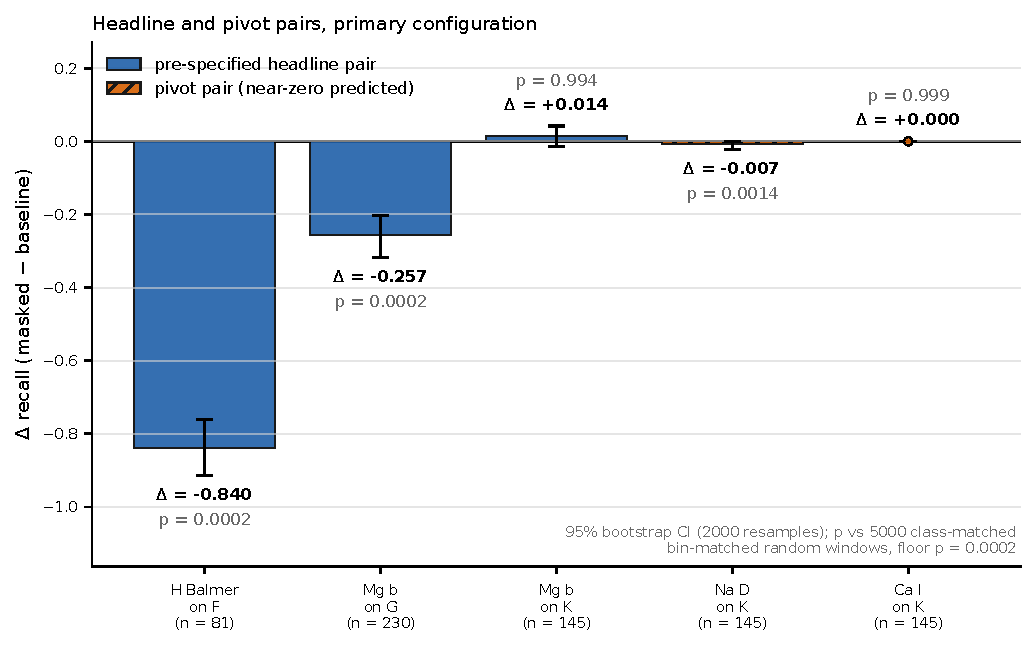
\includegraphics[width=0.85\linewidth]{ablation_bars.pdf}
\caption{Change in class recall $\dA_k^{(\mathcal{L})}$ for the headline (solid) and pivot (hatched) pairs in the primary configuration (production continuum, interpolation fill). Error bars are 95 percent bootstrap intervals (\ablNBoot{} resamples); each bar is annotated with $\dA$ and the Monte Carlo $p$-value against \ablNControls{} class-matched, bin-matched random windows (floor \ablFloor). The K bars are small but not exactly zero in rows (Section~\ref{subsec:kclass}); the values match Table~\ref{tab:ablation}.}
\label{fig:ablation}
\alttext{Bar chart of the change in class recall for five line-set and class pairs. Masking the Balmer windows drops F recall to zero and masking Mg b lowers G recall by about a quarter; the three pairs involving the K class are close to zero. Error bars show bootstrap intervals; headline pairs are solid bars and pivot pairs hatched.}
\end{figure*}

\subsection{The K class responds to no narrow window}
\label{subsec:kclass}

K-class recall barely changes under any of the five line sets (Table~\ref{tab:ablation-k}). Counting rows in the primary configuration, no line set loses more than \ablKMaxLost{} of the \nClassK{} K rows: \FeCr loses \ablPrimFeKLost{} and gains \ablPrimFeKGained{} (McNemar $p = \ablPrimFeKMcn$), (\Mgb, K) loses \ablPrimMgKLost{} and gains \ablPrimMgKGained{} ($p = \ablPrimMgKMcn$), (\NaD, K) loses \ablPrimNaKLost{} and gains \ablPrimNaKGained{} ($p = \ablPrimNaKMcn$), and (\CaI, K) loses \ablPrimCaKLost{} and gains \ablPrimCaKGained{}. The one-sided exact 95 percent upper bound on the loss rate is at most \ablKMaxUpper{} for any line set, \ablPrimMgKUpper{} for \Mgb and \NaD, and \ablPrimCaKUpper{} for \CaI. The largest decrease in K recall is \ablKMaxDrop. K recall can also rise: masking the Balmer lines gains \ablPrimHbKGained{} rows ($\dA_K = \ablPrimHbKDelta$, McNemar $p = \ablPrimHbKMcn$). This is the same temperature response as in Section~\ref{subsec:results-ablation}: a mask that makes a star look cooler can only add K rows, and the gain is not reliance of K on the masked region.

\emph{Why the Monte Carlo $p$ is not the K evidence.} For K the class-matched reference distribution is concentrated at zero: only \ablPrimNaKNullB{} of \ablNControls{} random \ablPrimNaKBins-bin windows lower K recall by as much as one row, so one lost row in (\NaD, K) ($\dA_K = \ablPrimNaKDelta$, McNemar $p = \ablPrimNaKMcn$) already gives $p_{\mathrm{MC}} = \ablPrimNaKP$. For (\FeCr, K) none of the random windows loses as many as \ablPrimFeKLost{} K rows (\ablPrimFeKNullB{} at least as extreme), so \ablPrimFeKLost{} lost rows sit at the floor, $p_{\mathrm{MC}} = \ablPrimFeKP$. These values say that the window is unusual among windows of its width, which is a statement about how rarely any window moves K, and not that the effect differs from zero. We therefore apply one standard to every K pair, namely flip counts, the exact McNemar test and the exact upper bound, and we do not call (\NaD, K) or (\FeCr, K) effects; the \FeCr result is suggestive at most.

For (\Mgb, K) the change is \ablPrimMgKDelta{} with interpolation (interval [\ablPrimMgKCiLo, \ablPrimMgKCiHi]) and \ablConstMgKDelta{} with the constant fill (\ablConstMgKLost{} lost, \ablConstMgKGained{} gained). Under polynomial\_n5 it is \ablPolyMgKDelta{} with interpolation (\ablPolyMgKLost{} lost, \ablPolyMgKGained{} gained; McNemar $p = \ablPolyMgKMcn$) and \ablPolyConstMgKDelta{} with the constant fill (\ablPolyConstMgKLost{} and \ablPolyConstMgKGained; $p = \ablPolyConstMgKMcn$). The McNemar test rejects in neither case, and the model is already degraded there. For (\CaI, K) under polynomial\_n5 the change is \ablPolyCaKDelta{} with $p_{\mathrm{MC}} = \ablPolyCaKP$. The defensible statement is that K predictions barely respond to any of the five line sets we masked (8 to 80~\AA{} total width). It is not evidence for a particular alternative route, and an upper bound is not a measurement of zero. The bounds also set the resolution of each null: with \ablPrimCaKLost, \ablPrimMgKLost{} or \ablPrimFeKLost{} of \nClassK{} rows lost the audit cannot exclude loss rates up to \ablPrimCaKUpper, \ablPrimMgKUpper{} and \ablKMaxUpper, so a K dependence below those rates would not register, and the \CaI and \NaD sets cover so few bins (\ablPrimCaKBins{} and \ablPrimNaKBins{} of \sdNBins) that a null there is close to guaranteed for a tree model with redundant features.

The \Mgb equivalent width on K spectra is not small: the median is \ewMedK~\AA{} against \ewMedG~\AA{} on G and \ewMedF~\AA{} on F (K minus G \ewDiff~\AA; KS $p = \ewKsP$). This rules out the explanation that the K \Mgb signal is too weak to matter, but \Mgb wings are a gravity indicator and the K sample is giant-dominated, so the comparison is confounded by luminosity (Section~\ref{subsec:lum}).

\emph{Positive control.} Narrow windows are not the only masks we tried (Table~\ref{tab:kcontrol}). Masking all five line sets jointly (\pcBinsJoint{} bins) leaves K recall unchanged or higher under both fills (\pcPrimJointKDelta{} with interpolation, \pcConstJointKDelta{} with the constant fill). Masking the \pcBinsTopHundred{} bins with the largest validation-set mean $|$SHAP$|$ for K (\pcBinsPctTopHundred{} percent of the spectrum in \pcWindowsTopHundred{} runs, carrying \pcShapShareTopHundred{} percent of the total K attribution) raises K recall by \pcPrimTopHundredKDelta{} with interpolation (\pcPrimTopHundredKGained{} rows gained, \pcPrimTopHundredKLost{} lost) but lowers it by \pcConstTopHundredKDelta{} with the constant fill (\pcConstTopHundredKLost{} of \nClassK{} rows lost, all to G, \pcConstTopHundredKGained{} gained; McNemar $p = \pcConstTopHundredKMcn$; upper bound on the loss rate \pcConstTopHundredKUpper), and the mean probability of the true class changes by \pcConstTopHundredKDp. The constant fill already moves that probability at 20 and 50 bins (\pcConstTopTwentyKDp{} and \pcConstTopFiftyKDp) before any row changes class. The two fills disagree because interpolating across the Balmer cores and the other K-ranked runs makes a spectrum look cooler: under the top-100 mask with interpolation, \pcPrimTopHundredFToK{} of the \pcPrimTopHundredFLost{} lost F rows and all \pcPrimTopHundredGLost{} lost G rows are relabelled K. Two conclusions follow. The ablation can register a K dependence when enough K-relevant bins are removed with a constant fill, so the null results for the five line sets are not an artefact of a readout that cannot see K; this control rests on one mask and one fill, however, since at \pcBinsTopTwenty{} and \pcBinsTopFifty{} bins the constant fill moves no K row on balance (\pcConstTopTwentyKLost{} lost and \pcConstTopTwentyKGained{} gained, then \pcConstTopFiftyKLost{} and \pcConstTopFiftyKGained), so the audit's power for K is demonstrated only at the scale of the \pcBinsTopHundred-bin mask. And with the interpolation fill no mask we tried lowers K recall, so ``K recall does not respond'' must be read as ``does not fall''. Interpolation does not push every spectrum toward the cooler class: under the \Mgb mask most lost G rows move to F, the hotter class (Section~\ref{subsec:results-ablation}). What holds for every mask we tried is narrower. Interpolating across the Balmer cores and the SHAP-ranked runs removes features that are stronger in hotter stars, so rows move toward K; interpolating across \Mgb removes a feature that is stronger in cooler stars, so rows move away from K, but only \ablPrimMgKLost{} K row leaves, because the K giants sit far from the 5300~K boundary. K is the sink for the first kind of mask and is insulated by boundary distance from the second.


\begin{table*}[ht]
\centering
\caption{K-class $\dA_K$ (rows lost/gained in brackets) for each line set under the 2 $\times$ 2 design: production or polynomial\_n5 continuum, each with interpolation (primary) or constant fill. The constant fill is the median of the training matrix outside the gap under the same continuum (\ablFillTrainProd{} for production, \ablFillTrainPoly{} for polynomial\_n5).}
\label{tab:ablation-k}
\small
\resizebox{\textwidth}{!}{% Generated by scripts/revision/manuscript_numbers.py from artifacts/revision/ablation_recalibrated.json
\begin{tabular}{lcccc}
\toprule
Line set & Prod., interp. & Prod., constant & Poly., interp. & Poly., constant \\
\midrule
H Balmer & \ensuremath{+0.055} (0/8) & \ensuremath{+0.028} (3/7) & \ensuremath{+0.076} (0/11) & \ensuremath{+0.076} (0/11) \\
Mg\,\textsc{b} & \ensuremath{+0.014} (1/3) & \ensuremath{0.000} (1/1) & \ensuremath{-0.014} (3/1) & \ensuremath{-0.034} (6/1) \\
Na\,\textsc{d} & \ensuremath{-0.007} (1/0) & \ensuremath{-0.007} (1/0) & \ensuremath{+0.007} (0/1) & \ensuremath{+0.007} (0/1) \\
Ca\,\textsc{i} & \ensuremath{0.000} (0/0) & \ensuremath{0.000} (0/0) & \ensuremath{-0.007} (1/0) & \ensuremath{-0.007} (1/0) \\
Fe\,\textsc{i}/Cr\,\textsc{i} & \ensuremath{-0.021} (3/0) & \ensuremath{-0.021} (3/0) & \ensuremath{-0.014} (2/0) & \ensuremath{-0.028} (4/0) \\
\bottomrule
\end{tabular}
}
\end{table*}

\begin{table*}[ht]
\centering
\caption{K-class positive control: $\dA_K$ for the joint mask of all five line sets and for the 20, 50 and 100 bins with the largest validation-set mean $|$SHAP$|$ for class K, under the interpolation and constant fills (production continuum, class-matched null of \pcNControls{} bin-matched windows, \pcNBoot{} bootstrap resamples). ``Upper bound'' is the one-sided exact 95 percent Clopper--Pearson bound on the loss rate. The SHAP-ranked sets are post hoc; \pcOverlapTopHundred{} of the 100 bins lie inside the catalogued windows.}
\label{tab:kcontrol}
\small
\resizebox{\textwidth}{!}{% Generated by scripts/revision/manuscript_numbers.py from artifacts/revision/k_positive_control.json
\begin{tabular}{llrrcrrr}
\toprule
Mask & Fill & Bins & $\dA_K$ [95\% CI] & Flips (l/g) & $p_{\mathrm{McN}}$ & Upper bound & $\Delta\bar{P}_{\mathrm{true}}$ \\
\midrule
All five sets jointly & interpolation & 56 & \ensuremath{+0.055} \ensuremath{[+0.020, +0.093]} & 0/8 & \ensuremath{0.0078} & \ensuremath{0.020} & \ensuremath{+0.054} \\
 & constant & 56 & \ensuremath{+0.014} \ensuremath{[-0.027, +0.054]} & 4/6 & \ensuremath{0.754} & \ensuremath{0.062} & \ensuremath{-0.054} \\
\addlinespace
Top-20 K $|$SHAP$|$ bins & interpolation & 20 & \ensuremath{+0.055} \ensuremath{[+0.021, +0.096]} & 0/8 & \ensuremath{0.0078} & \ensuremath{0.020} & \ensuremath{+0.037} \\
 & constant & 20 & \ensuremath{+0.021} \ensuremath{[-0.020, +0.063]} & 3/6 & \ensuremath{0.508} & \ensuremath{0.053} & \ensuremath{-0.051} \\
\addlinespace
Top-50 K $|$SHAP$|$ bins & interpolation & 50 & \ensuremath{+0.041} \ensuremath{[+0.007, +0.080]} & 1/7 & \ensuremath{0.070} & \ensuremath{0.032} & \ensuremath{+0.034} \\
 & constant & 50 & \ensuremath{0.000} \ensuremath{[-0.043, +0.041]} & 5/5 & \ensuremath{1.000} & \ensuremath{0.071} & \ensuremath{-0.127} \\
\addlinespace
Top-100 K $|$SHAP$|$ bins & interpolation & 100 & \ensuremath{+0.062} \ensuremath{[+0.026, +0.106]} & 0/9 & \ensuremath{0.0039} & \ensuremath{0.020} & \ensuremath{+0.055} \\
 & constant & 100 & \ensuremath{-0.166} \ensuremath{[-0.232, -0.106]} & 25/1 & \ensuremath{8.0\times10^{-7}} & \ensuremath{0.232} & \ensuremath{-0.339} \\
\bottomrule
\end{tabular}
}
\end{table*}

\subsection{The luminosity-class confound}
\label{subsec:lum}

The K class is mostly giants and the F and G classes are almost all dwarfs (Table~\ref{tab:lum}, Figure~\ref{fig:kiel}). In the full sample \lumDwarfPctF{} percent of F rows, \lumDwarfPctG{} percent of G rows and \lumDwarfPctK{} percent of K rows have $\log g > \lumLoggCut$, with median $\log g$ of \lumLoggF, \lumLoggG{} and \lumLoggK. On the test set the model scores \lumAccKGiant{} on K giants ($n = \lumAccNKGiant$) and \lumAccKDwarf{} on K dwarfs ($n = \lumAccNKDwarf$); it scores \lumAccGDwarf{} on G dwarfs ($n = \lumAccNGDwarf$) and \lumAccGGiant{} on G giants ($n = \lumAccNGGiant$). The \gkErrN{} G rows predicted K include \gkErrDwarf{} dwarfs; their median $\log g$ is \gkErrLogg{} and median \Teff \gkErrTeff~K. ``K against G'' is therefore partly ``giant against dwarf''. The labels are \Teff bins on a dwarf scale, so ``K'' here means a \Teff bin that is mostly populated by red giants.

K rows also lie far from the class boundaries: the median distance to the nearest edge of the row's own \Teff bin is \bdMedK~K for K against \bdMedF{} for F and \bdMedG{} for G, and only \bdNearK{} of \nClassK{} K rows lie within \bdCut~K of an edge. Accuracy within that distance is \bdAccNearK{} for K and beyond it \bdAccFarK. Measuring the distance only to the shared 5300 and 6000~K boundaries gives a K median of \focusKMedInterior~K and \focusKNearInterior{} rows within \bdCut~K; the F and G values do not change. A push toward a hotter or cooler prediction, which is what masking a line does to a temperature estimator, rarely carries a K row across a boundary, which limits what an unchanged K recall can mean.

Table~\ref{tab:strata} (Appendix~\ref{app:figures}) splits the principal pairs by luminosity class and by boundary distance. For F and G the luminosity split is uninformative, since only three F rows and one G row are giants. Under \Mgb masking, \focusMgGDwarf{} of the \focusMgGLost{} lost G rows are dwarfs, and the loss is concentrated near the boundaries: $\dA_G = \strMgGNearDelta$ for the \strMgGNearN{} G rows within \bdCut~K of an edge of their bin against \strMgGFarDelta{} beyond it, and \focusMgGNear{} of the lost rows lie within that distance. For K, every row that changes class is a dwarf: across the five line sets \kLostDistinct{} distinct K rows are lost, \kLostDwarf{} of them dwarfs and \kLostNear{} within \bdCut~K of an edge, while K giants ($n = \lumAccNKGiant$) lose \kGiantLost{} and gain \kGiantGained{} rows. The K gains under Balmer masking are also dwarfs (\strHbKDwarfGained{} rows, $\dA_K = \strHbKDwarfDelta$ among the \strHbKDwarfN{} K dwarfs). The apparent insensitivity of the K class is therefore largely the insensitivity of its giants, which never change class under any of the five line sets; the \pcBinsTopHundred-bin constant-fill mask of Section~\ref{subsec:kclass} is the one mask that does move K giants.

\begin{table*}[ht]
\centering
\caption{Composition and test accuracy by luminosity class. Dwarfs have $\log g > \lumLoggCut$. Fractions are over the full labelled sample; accuracies are on the held-out test rows (counts in brackets).}
\label{tab:lum}
\small
\setlength{\tabcolsep}{4pt}
\fittable{\begin{tabular}{lrrrrcc}
\toprule
Class & $n$ & Dwarf (\%) & Median $\log g$ & Median \Teff (K) & Test acc., dwarfs & Test acc., giants \\
\midrule
F & \lumNF & \lumDwarfPctF & \lumLoggF & \lumTeffF & \lumAccFDwarf{} (\lumAccNFDwarf) & \lumAccFGiant{} (\lumAccNFGiant) \\
G & \lumNG & \lumDwarfPctG & \lumLoggG & \lumTeffG & \lumAccGDwarf{} (\lumAccNGDwarf) & \lumAccGGiant{} (\lumAccNGGiant) \\
K & \lumNK & \lumDwarfPctK & \lumLoggK & \lumTeffK & \lumAccKDwarf{} (\lumAccNKDwarf) & \lumAccKGiant{} (\lumAccNKGiant) \\
\bottomrule
\end{tabular}}
\end{table*}

\begin{figure}[ht]
\centering
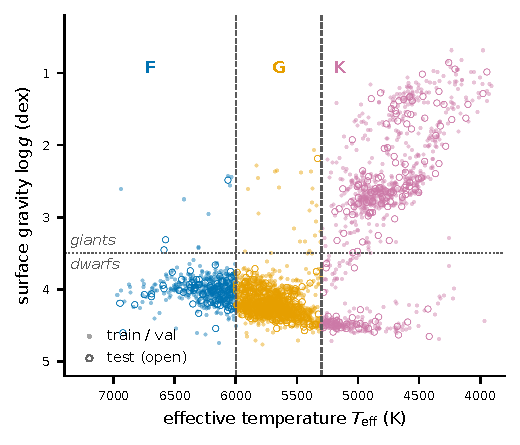
\includegraphics[width=0.8\linewidth]{kiel_diagram.pdf}
\caption{Kiel diagram of the labelled sample coloured by class. The F and G classes lie on the dwarf branch and the K class is dominated by giants; the dwarf cut is $\log g = \lumLoggCut$.}
\label{fig:kiel}
\alttext{Scatter plot of surface gravity against effective temperature for the labelled sample, coloured by class. F and G stars lie on the high-gravity dwarf branch at the hotter temperatures; most K stars lie on the low-gravity giant branch at cooler temperatures, with a smaller group of K dwarfs. A horizontal line marks the dwarf cut.}
\end{figure}

\subsection{Scale mismatch under polynomial re-normalisation}
\label{subsec:scale}

Re-deriving the continuum of the test rows with a sigma-clipped polynomial lowers G recall from \sdProdRecG{} to \sdPolyRecG{} and macro-F1 from \sdProdMacroF{} to \sdPolyMacroF, with \sdGtoKPoly{} of \nClassG{} G rows moving to K and \sdPolyGtoF{} to F (Table~\ref{tab:scale}). The re-normalisation changes two things at once: it removes the class-dependent level spread, and it lifts the global median level from \sdMedProdGlobal{} to \sdMedPolyGlobal, about \sdPolyShiftPct{} percent. Gradient-boosted trees split on absolute thresholds, so a level shift can move every bin across a split. The decomposition with the model held fixed separates the two effects (Table~\ref{tab:scale}, Figure~\ref{fig:continuum_medians}).

\begin{itemize}
\item Removing the spread while keeping the scale (every row rescaled to the common test median) costs \sdCostCommon{} in macro-F1 (to \sdCommonMacroF) and leaves \sdCommonGtoK{} G rows going to K.
\item Keeping the spread and shifting the scale (every row multiplied by \sdUniMult) approximately reproduces the collapse: macro-F1 \sdUniNineMacroF, G recall \sdUniNineRecG, and \sdUniNineGtoK{} G rows going to K. The ratio of the global medians, \sdBestMult, gives \sdUniBestMacroF{} and \sdUniBestGtoK{} rows.
\item Swapping the G and K median levels costs \sdCostSwap{} and raises G$\to$K to \sdSwapGtoK.
\item Restoring the production values of the gap bins after re-normalisation changes macro-F1 by less than 0.005 (\sdPolyGapMacroF{} against \sdPolyMacroF), so the gap bins do not carry the effect.
\end{itemize}
The level itself holds weak class information. A one-feature logistic regression on the per-row off-gap median reaches accuracy \oneAcc{} (balanced accuracy \oneBal) on the test set, with ROC AUC \oneAucGK{} for G against K and \oneAucFG{} for F against G. The per-class median of the row medians is \medProdF{} (F), \medProdG{} (G) and \medProdK{} (K) under the production normalisation, a spread of \spreadProd{} percentage points before rounding, with KS $p$ of \ksProdFG{} (F--G), \ksProdGK{} (G--K) and \ksProdFK{} (F--K). After the polynomial fit the medians are \medPolyF, \medPolyG{} and \medPolyK{} (a spread of \spreadPoly{} points, with the order reversed), and the KS $p$ are \ksPolyFG, \ksPolyGK{} and \ksPolyFK. The level carries real but weak class information, but a model that read only the level could not reach G recall of \sdProdRecG, and after re-normalisation all three class medians lie above the production F median, so a model that read the level would be expected to move G toward F rather than K. We conclude that the polynomial collapse is a train--test scale mismatch: the model has not seen the scale of the re-normalised inputs. This is brittleness to a normalisation convention, which is a failure to transfer to a shifted condition. We do not identify a specific unintended feature the model relies on, and we therefore do not call it shortcut learning.

\begin{table*}[ht]
\centering
\caption{The fixed production model scored on transformed test spectra. Recall per class, macro-F1 and the number of G rows predicted K, with the median row level in the last column. ``Spread removed'' rescales each row to the common test median; ``G/K swap'' exchanges the two class median levels.}
\label{tab:scale}
\small
\fittable{\begin{tabular}{lrrrrrr}
\toprule
Transformation & $R_F$ & $R_G$ & $R_K$ & macro-F1 & G$\to$K & Median level \\
\midrule
Production & \sdProdRecF & \sdProdRecG & \sdProdRecK & \sdProdMacroF & \sdProdGtoK & \sdProdLevel \\
Polynomial\_n5 & \sdPolyRecF & \sdPolyRecG & \sdPolyRecK & \sdPolyMacroF & \sdPolyGtoK & \sdPolyLevel \\
Polynomial\_n5, gap restored & \sdPolyGapRecF & \sdPolyGapRecG & \sdPolyGapRecK & \sdPolyGapMacroF & \sdPolyGapGtoK & \sdPolyGapLevel \\
Spread removed, scale kept & \sdCommonRecF & \sdCommonRecG & \sdCommonRecK & \sdCommonMacroF & \sdCommonGtoK & \sdCommonLevel \\
Every row $\times$ \sdUniMult & \sdUniNineRecF & \sdUniNineRecG & \sdUniNineRecK & \sdUniNineMacroF & \sdUniNineGtoK & \sdUniNineLevel \\
Every row $\times$ \sdBestMult & \sdUniBestRecF & \sdUniBestRecG & \sdUniBestRecK & \sdUniBestMacroF & \sdUniBestGtoK & \sdUniBestLevel \\
G/K swap & \sdSwapRecF & \sdSwapRecG & \sdSwapRecK & \sdSwapMacroF & \sdSwapGtoK & \sdSwapLevel \\
\bottomrule
\end{tabular}}
\end{table*}

\begin{figure*}[ht]
\centering
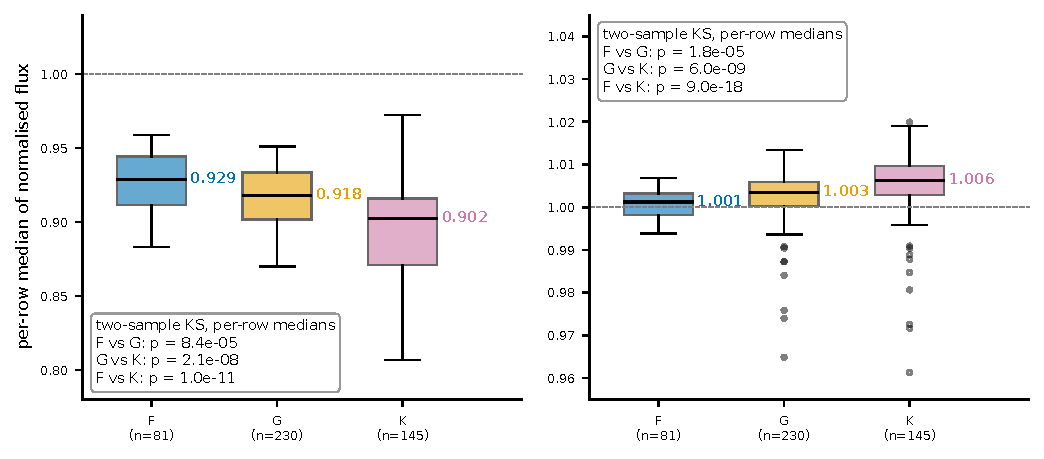
\includegraphics[width=0.92\linewidth]{continuum_medians.pdf}
\caption{Per-row median of normalised flux outside the inter-chip gap by class on the test set, under the production normalisation (left) and after the polynomial re-normalisation (right). Class medians are given in Section~\ref{subsec:scale}; the numbers come from the same artifact as Table~\ref{tab:scale}. The two panels use different vertical ranges.}
\label{fig:continuum_medians}
\alttext{Two box-plot panels of the per-row median normalised flux for the F, G and K test spectra. Under the pipeline normalisation (left) the class medians fall from F to G to K, all below unity. After polynomial re-normalisation (right) all three medians sit just above unity, in the reverse order and with a much smaller spread.}
\end{figure*}

\subsection{Retraining on re-normalised spectra}
\label{subsec:retrain}

We ran the retraining experiment that tests whether the K result depends on the continuum convention (Table~\ref{tab:retrain}). The production retrain reproduces the deposited model exactly (macro-F1 difference \rtReproDiff, identical confusion matrix, best iteration \rtProdIter). Retrained on polynomial\_n5 features the model reaches macro-F1 \rtPolyMacroF{} and on row-median-normalised features \rtRowMedMacroF, a loss of \rtDeltaMacroPoly{} and \rtDeltaMacroRow{} against the production \rtProdMacroF. This is within the fold-to-fold spread of 5-fold cross-validation on the production matrix (\cvMean{} with population standard deviation \cvSd; Section~\ref{subsec:cv}). The classifier loses about a hundredth of macro-F1 without the level, so the level is not what carries performance. In every retrained model the (\Mgb, K) change is null or slightly positive (\rtProdMgKDelta, \rtPolyMgKDelta, \rtPolyGapMgKDelta, \rtRowMedMgKDelta{} for the four matrices), while (\Mgb, G) is clearly negative (\rtProdMgGDelta, \rtPolyMgGDelta, \rtPolyGapMgGDelta, \rtRowMedMgGDelta). The change in K recall seen when the fixed model scores polynomial-normalised inputs (\ablPolyMgKDelta{} with interpolation and \ablPolyConstMgKDelta{} with the constant fill; Table~\ref{tab:ablation-k}) is therefore a response of a model scored far from its training conditions (baseline accuracy \ablBaseAccPoly), not a property of the K class. The retraining was first planned as future work; because the same rows train, validate and test, it does not invalidate the split. The \Mgb results do not depend on the normalisation convention; Section~\ref{subsec:robustness} varies the training choices instead.

\begin{table*}[ht]
\centering
\caption{LightGBM retrained with the production hyperparameters on each feature matrix (same train/validation/test rows). Recall per class, macro-F1, G rows predicted K, and the \Mgb ablation on K and G (constant fill at the test-matrix median, the deposited convention of this experiment, whereas Tables~\ref{tab:ablation} and~\ref{tab:ablation-k} use the training median; class-matched null, \rtNControls{} windows, \rtNBoot{} bootstrap resamples; the null for this table forbids only the \Mgb bins and the gap when drawing windows, whereas Table~\ref{tab:ablation} forbids every catalogued window). Intervals are 95 percent bootstrap intervals.}
\label{tab:retrain}
\footnotesize
\resizebox{\textwidth}{!}{%
\begin{tabular}{lrrrrrcc}
\toprule
Features & $R_F$ & $R_G$ & $R_K$ & macro-F1 & G$\to$K & $\dA_K$ (\Mgb) [95\%] ($p_{\mathrm{MC}}$) & $\dA_G$ (\Mgb) [95\%] ($p_{\mathrm{MC}}$) \\
\midrule
Production & \rtProdRecF & \rtProdRecG & \rtProdRecK & \rtProdMacroF & \rtProdGtoK & \rtProdMgKDelta{} [\rtProdMgKCiLo, \rtProdMgKCiHi] (\rtProdMgKP) & \rtProdMgGDelta{} [\rtProdMgGCiLo, \rtProdMgGCiHi] (\rtProdMgGP) \\
Polynomial\_n5 & \rtPolyRecF & \rtPolyRecG & \rtPolyRecK & \rtPolyMacroF & \rtPolyGtoK & \rtPolyMgKDelta{} [\rtPolyMgKCiLo, \rtPolyMgKCiHi] (\rtPolyMgKP) & \rtPolyMgGDelta{} [\rtPolyMgGCiLo, \rtPolyMgGCiHi] (\rtPolyMgGP) \\
Polynomial\_n5, gap restored & \rtPolyGapRecF & \rtPolyGapRecG & \rtPolyGapRecK & \rtPolyGapMacroF & \rtPolyGapGtoK & \rtPolyGapMgKDelta{} [\rtPolyGapMgKCiLo, \rtPolyGapMgKCiHi] (\rtPolyGapMgKP) & \rtPolyGapMgGDelta{} [\rtPolyGapMgGCiLo, \rtPolyGapMgGCiHi] (\rtPolyGapMgGP) \\
Row-median & \rtRowMedRecF & \rtRowMedRecG & \rtRowMedRecK & \rtRowMedMacroF & \rtRowMedGtoK & \rtRowMedMgKDelta{} [\rtRowMedMgKCiLo, \rtRowMedMgKCiHi] (\rtRowMedMgKP) & \rtRowMedMgGDelta{} [\rtRowMedMgGCiLo, \rtRowMedMgGCiHi] (\rtRowMedMgGP) \\
\bottomrule
\end{tabular}}
\end{table*}

\subsection{Robustness of the (\texorpdfstring{\Mgb}{Mg b}, K) effect to training choices}
\label{subsec:robustness}

Two further retrains were run on the production features with the deposited constant fill. With uniform class weights the model reaches macro-F1 \uwMacroF{} and the (\Mgb, K) change is \uwDelta. Across a $3 \times 3$ grid of \texttt{max\_depth} $\in \{6, 8, 10\}$ and \texttt{num\_leaves} $\in \{31, 63, 127\}$ (\gridNCells{} cells) the largest absolute change is \gridMaxDelta. The grid does not vary the learning rate, the column subsampling, the objective or the regularisation, so this is a statement about those nine cells and not about gradient-boosted trees in general.

\section{Discussion}
\label{sec:discussion}

\paragraph{What the audit adds.} A list of line windows fixed in advance, a per-class readout and a class-matched, bin-matched null make the answer to ``does this classifier depend on this window for this class'' reproducible, and the flip counts and McNemar test make the K-class statement honest about how few rows move. The method is an operation on the input domain of a fixed model and is model-agnostic in principle, although we have applied it to one model. It does not separate a physical dependence from a response to an edited input, since masking and interpolation can leave the data manifold \citep{Hooker2019Benchmark,Covert2021Removing}, and it measures reliance on a window, not the causal effect of a stellar property. The prior-art approaches that build the dependence structure into the model \citep{2019ApJ...879...69T,2019ApJS..245...34X,2019MNRAS.483.3255L} answer a different question: how to constrain a model, where we probe an unconstrained one.

\paragraph{Attribution baselines and ablation.} The three baselines of Section~\ref{subsec:triangulation} point at the Balmer and \Mgb regions and disagree elsewhere. A ranking says where the model looks; only the intervention says whether the prediction changes when the region is edited, and K-class insensitivity is a property of that response. The scale mismatch is not an attribution result at all: it appears when the per-class level and the global scale of the inputs are examined directly.

\paragraph{The scale mismatch.} A reading in which the model used the per-class continuum level as its main G-versus-K discriminator fails three tests. A uniform rescaling that keeps the spread approximately reproduces the collapse (macro-F1 \sdUniNineMacroF{} against \sdPolyMacroF, so a small reliance on the level is not excluded); removing the spread while keeping the scale does not reproduce it; and retraining without the level costs about a hundredth of macro-F1. That a tree ensemble fails under a uniform rescaling of its inputs is dataset shift in the sense of \citet{QuinoneroCandela2009Shift}, here a deterministic transformation of the inputs that moves their distribution while the physical labelling rule stays fixed: trees split on absolute thresholds, so nothing in the model carries over across a change of scale, and the contribution here is the decomposition, not the phenomenon. The closest stellar-spectroscopy precedents are the mismatch between synthetic training spectra and observed spectra documented by \citet{2020MNRAS.498.3817B} and the domain adaptation it motivated \citep{2021ApJ...906..130O}; the shift here is smaller and purely multiplicative, which is what makes it easy to miss. For pipeline-normalised spectra the practical lesson is that a tree model scored on a re-normalised matrix, even by a small uniform shift, should be treated as scored on shifted inputs. We recommend reporting the normalisation convention, the global median level, and a uniform-rescaling sensitivity check alongside any such evaluation.

\paragraph{What the K result does and does not say.} K recall does not respond to any narrow window: K giants, which are \lumAccNKGiant{} of the \nClassK{} K test rows, lose \kGiantLost{} and gain \kGiantGained{} rows under all five masks. The class is giant-dominated, sits far from the class edges, and has many redundant temperature-sensitive features, so a narrow mask removes little that other bins cannot supply. The positive control of Section~\ref{subsec:kclass} sharpens this in two directions: a constant fill over the \pcBinsTopHundred{} most K-relevant bins does lower K recall (by \pcConstTopHundredKDelta), so the audit can see a K dependence once enough redundant bins are removed, while the interpolation fill never lowers K recall for any mask we tried, because the masks that remove hotter-star features move rows toward K and the one that removes a cooler-star feature (\Mgb) moves almost no K row across the distant 5300~K boundary (Section~\ref{subsec:kclass}). The K statement is therefore conditional on the fill as well as on the width of the mask. We do not infer a shortcut from any of this, and the \FeCr result is suggestive at most. Comparing with an external parameter-inference network such as that of \citet{2024A&A...692A.228C} is not informative here, since it is a different task on a different instrument.

\section{Limitations}
\label{sec:limitations}

\textbf{Labels and luminosity.} The classes are \Teff bins from parameters derived from the same spectra, on a dwarf scale, and the K class is giant-dominated. The audit tests reproduction of a spectroscopic \Teff bin, and no claim about MK classification in the full spectral and luminosity sense follows. Restricting the audit to dwarfs would leave only \lumNDwarfKtest{} K test rows.

\textbf{Resolution and blends.} The bins correspond to $R \approx 2000$, so a line window is a blend (Table~\ref{tab:linesets}) and the native UVES resolving power is not used by the features. The \Mgb window contains \FeI lines, and ``\Mgb dependence'' means dependence on that 21~\AA{} region. The window widths differ by a factor of about ten, from 8 to 80~\AA, which is why the nulls are matched in bin count and drawn per class.

\textbf{Interventions.} Interpolation and constant fills are off-distribution edits. The ablation is on a single model, one instrument and one survey, with the GES parameters as labels. Effects based on a few rows do not support claims beyond the sample. The indifference zone was chosen after the data were seen and is descriptive.

\textbf{Labels, noise and imbalance.} Of the test rows, \bdNearF{} F, \bdNearG{} G and \bdNearK{} K lie within \bdCut~K of a class edge, a distance of the same order as the per-star \Teff uncertainties quoted in the homogenised catalogue \citep{2023A&A...676A.129H}, and accuracy beyond \bdThresh~K of an edge is \bdFiltAcc{} against \bdFullAcc{} overall (Section~\ref{subsec:perf}), so almost every error is a boundary row whose label is itself uncertain at the level of the bin edge. The classes are imbalanced (test F = \nClassF, G = \nClassG, K = \nClassK; balanced class weights in training) and the K dwarfs number only \lumNDwarfKtest{} in the test set, which limits every per-stratum statement about them.

\textbf{Leakage and spatial structure.} Because \singRowPct{} percent of train+val rows are in singleton spatial groups, the DBSCAN pass does not constrain cluster leakage; the pass grouped by survey field differs from the plain estimate by \cvFldGapPlain{} of macro-F1, below the \cvGap{} split-to-split spread of a single five-fold run, so no field-mate leakage is detectable at that resolution, and repeating both passes over many seeds would be needed to measure a smaller effect (Section~\ref{subsec:cv}). The held-out test split itself is not group-aware, so test rows can share a field with training rows, and the test score should be read with the field-grouped estimate beside it. The DBSCAN group identifiers are re-derived, not deposited; the field identifiers are deposited.

\textbf{External check.} The template cross-check failed its gate and so offers no corroboration (Appendix~\ref{app:pickles}).

\section{Conclusions}
\label{sec:conclusions}

A LightGBM classifier of three \Teff-bin classes on Gaia-ESO UVES U580 spectra reaches macro-F1 \testMacroF. Under masked-line ablation with line windows fixed in advance and class assignments frozen before the ablation was read (Section~\ref{subsec:deviations}), the F and G classes cannot tolerate removal of the Balmer windows and the G class depends on the \Mgb region: masking them changes recall by \ablPrimHbFDelta{} and \ablPrimMgGDelta{} (\ablPrimHbFLost{} and \ablPrimMgGLost{} rows lost, \ablPrimMgGGained{} gained for \Mgb). Under the \Mgb mask rows move as a temperature estimator would move them; under the Balmer masks no row is predicted F at all, and F rows go straight to K. The size of the Balmer effect and the destination of its errors depend on the fill; the \Mgb effect does not (\ablConstMgGDelta{} with the constant fill). The K class does not lose recall under any narrow window we tried: in the primary configuration no line set loses more than \ablKMaxLost{} of \nClassK{} K rows, and masks that make a star look cooler add K rows. With the interpolation fill no mask, not even the \pcBinsTopHundred{} most K-relevant bins, lowers K recall; with a constant fill that mask does (\pcConstTopHundredKDelta), so the audit can register a K dependence once one is removed. That is the full content of the K result. Its evidence is flip counts, exact McNemar tests and upper bounds, since the Monte Carlo $p$-values are near-degenerate for K, and it is a failure to detect a narrow-window dependence in a giant-dominated class, not a finding about what the K class reads instead. A class-level continuum shortcut is not supported: the collapse under polynomial re-normalisation is a train--test scale mismatch that a uniform \sdUniMult{} rescaling approximately reproduces, and retraining on re-normalised spectra restores the classifier and leaves the \Mgb effect on K null. For anyone scoring a tree model on re-normalised spectra the caution is practical: report the normalisation convention and the global level, and check sensitivity to a uniform rescaling. The code, model, feature matrix, decision log and every number-producing script are released so that the same probe can be run on other classifiers.

\section*{Data availability}

Code is available at \url{https://github.com/TirtheshJani/ges-uves-mk-audit} under the MIT licence. The trained model (\texttt{lgbm\_mk.pkl}), the feature matrix (\texttt{features.npz}) and the numerical artifacts are deposited at Zenodo (DOI to be minted from the v1.2.0 GitHub release through the Zenodo integration) with the same release tag as the GitHub repository. Reproduction commands, seeds and run times are in \path{docs/reproducibility_appendix.md}; the provenance of the three local copies of the project is in \path{docs/folder_provenance.md} and the dated decision log is \path{docs/decision_log.md}. Every number in this paper is written to \path{submission/revision_numbers.tex} by \path{scripts/revision/manuscript_numbers.py}, and \path{artifacts/revision/manuscript_numbers_index.json} maps each macro to its source artifact; the field identifiers, the field-grouped cross-validation and the K-class positive control are in \path{artifacts/revision/}. The Gaia-ESO data are public through the ESO Science Archive Facility. The Pickles library is public through the STScI HLSP reference-atlases mirror and is not redistributed.

\section*{Acknowledgements}

This work uses data from the Gaia-ESO Public Spectroscopic Survey \citep{2022A&A...666A.120G,2022A&A...666A.121R,2014A&A...565A.113S}. Based on data products from observations made with ESO Telescopes at the La Silla Paranal Observatory under programme ID 188.B-3002. Based on data obtained from the ESO Science Archive Facility with DOI: \url{https://doi.org/10.18727/archive/25}. These data products have been processed by the Cambridge Astronomy Survey Unit (CASU) at the Institute of Astronomy, University of Cambridge, and by the FLAMES/UVES reduction team at INAF/Osservatorio Astrofisico di Arcetri. Stellar parameters used for the labels are from \citet{2023A&A...676A.129H}. Atomic line rest wavelengths are from the NIST Atomic Spectra Database \citep{NIST_ASD_2023}. The Pickles library was retrieved from the STScI HLSP reference-atlases mirror. Software includes LightGBM \citep{Ke2017LightGBM}, SHAP \citep{LundbergLee2017SHAP,Lundberg2020TreeSHAP}, scikit-learn \citep{Pedregosa2011sklearn}, NumPy \citep{Harris2020numpy}, SciPy \citep{Virtanen2020scipy}, Astropy \citep{Astropy2022}, astroquery \citep{Ginsburg2019astroquery} and Matplotlib \citep{Hunter2007matplotlib}.

\section*{Conflict of interest}

The author declares no conflict of interest.

\section*{Funding}

The author declares no funding.

\section*{Author contributions}

Tirthesh Jani: conceptualization, methodology, software, validation, formal analysis, investigation, data curation, writing (original draft), writing (review and editing), visualization.

\section*{Declaration of generative AI and AI-assisted technologies in the writing process}

During the preparation of this work the author used large-language-model assistants to draft and refactor analysis code, to run internal review passes on earlier drafts and to copy-edit the text. After using these tools, the author reviewed and edited the content as needed; the study design, every analysis and every number in the paper were checked by the author, who takes full responsibility for the content of the publication.

\bibliographystyle{elsarticle-harv}
\bibliography{manuscript_citations}

\appendix

\section{External cross-check against the Pickles library: not passed}
\label{app:pickles}

No continuum convention reached the pre-specified agreement gate, so the cross-check is reported as a failed external check, not as corroboration. We compared each test spectrum with the \pkNTemplates{} spectra of the Pickles UVKLIB library \citep{1998PASP..110..863P} by minimising a unit-variance chi-squared over bins finite in both spectra, and compared the spectral type of the best template (read from the \texttt{COMMENT1} card of its FITS header, which agrees with the embedded map for \pkEmbedAgree{} of \pkNTemplates{} templates) with the classifier's prediction; an earlier hand-built index map was mis-assigned from index 17 onward and its results are withdrawn. The gate was agreement of at least \pkGate{} on at least \pkGateMinN{} compared rows. Table~\ref{tab:pickles} gives the result: the best agreement, \pkAgreeMfTwo{} for the 200~\AA{} median-filter normalisation, is below the gate, and for that normalisation \pkSuperMfTwo{} percent of best-matching templates are supergiants, a luminosity class essentially absent from the test sample. The polynomial\_n5 convention yields no F, G or K template matches, and the variant fitted on the 4700 to 6900~\AA{} window reaches only \pkAgreePolyWin. A template library without luminosity or metallicity matching to the sample cannot test a three-class \Teff classifier at this resolution, and we have not tried to repair it.

\begin{table}[ht]
\centering
\caption{Agreement between the classifier and the spectral type of the best-matching Pickles template under four continuum conventions (gate: agreement $\ge \pkGate$ and at least \pkGateMinN{} compared rows). ``Super.'' is the fraction of best-matching templates that are supergiants. The polynomial\_n5 convention gives no F, G or K matches. The last row is an additional variant fitted on a restricted window and is not part of the pre-specified set.}
\label{tab:pickles}
\fittable{\begin{tabular}{lrrrr}
\toprule
Convention & $n_{\mathrm{FGK}}$ & Agreement & Macro-F1 & Super. (\%) \\
\midrule
200~\AA{} median filter & \pkNMfTwo & \pkAgreeMfTwo & \pkMacroMfTwo & \pkSuperMfTwo \\
50~\AA{} median filter & \pkNMfFifty & \pkAgreeMfFifty & \pkMacroMfFifty & \pkSuperMfFifty \\
Polynomial $n=5$ (sigma-clipped) & \pkNPolyN & \pkAgreePolyN & \pkMacroPolyN & \pkSuperPolyN \\
Polynomial $n=5$, 4700--6900~\AA{} window & \pkNPolyWin & \pkAgreePolyWin & \pkMacroPolyWin & \pkSuperPolyWin \\
\bottomrule
\end{tabular}}
\end{table}

\appendixbreak
\section{Supplementary table and figures}
\label{app:figures}

Table~\ref{tab:strata} gives the stratified ablation referenced in Section~\ref{subsec:lum}; Figures~\ref{fig:importance} and~\ref{fig:confusion} give the attribution traces and the confusion matrix referenced in Section~\ref{subsec:perf}.

\begin{table*}[ht]
\centering
\caption{Ablation of the principal pairs by luminosity class and by distance to the nearest edge of the row's own \Teff bin (primary configuration). A dash marks an empty stratum.}
\label{tab:strata}
\small
\resizebox{\textwidth}{!}{% Generated by scripts/revision/manuscript_numbers.py from artifacts/revision/ablation_stratified.json
\begin{tabular}{llrrcr}
\toprule
Pair & Stratum & $n$ & $\dA$ [95\% CI] & Flips (l/g) & $\Delta\bar{P}_{\mathrm{true}}$ \\
\midrule
H Balmer, F & dwarfs & 78 & \ensuremath{-0.859} \ensuremath{[-0.936, -0.782]} & 67/0 & \ensuremath{-0.813} \\
 & giants & 3 & \ensuremath{-0.333} \ensuremath{[-1.000, +0.000]} & 1/0 & \ensuremath{-0.505} \\
 & $\leq 150$ K from boundary & 34 & \ensuremath{-0.706} \ensuremath{[-0.853, -0.559]} & 24/0 & \ensuremath{-0.667} \\
 & $> 150$ K from boundary & 47 & \ensuremath{-0.936} \ensuremath{[-1.000, -0.851]} & 44/0 & \ensuremath{-0.898} \\
\addlinespace
H Balmer, G & dwarfs & 229 & \ensuremath{-0.921} \ensuremath{[-0.952, -0.886]} & 211/0 & \ensuremath{-0.795} \\
 & giants & 1 & \ensuremath{0.000} \ensuremath{[+0.000, +0.000]} & 0/0 & \ensuremath{-0.305} \\
 & $\leq 150$ K from boundary & 72 & \ensuremath{-0.806} \ensuremath{[-0.889, -0.708]} & 58/0 & \ensuremath{-0.651} \\
 & $> 150$ K from boundary & 158 & \ensuremath{-0.968} \ensuremath{[-0.994, -0.937]} & 153/0 & \ensuremath{-0.857} \\
\addlinespace
H Balmer, K & dwarfs & 38 & \ensuremath{+0.211} \ensuremath{[+0.079, +0.342]} & 0/8 & \ensuremath{+0.181} \\
 & giants & 107 & \ensuremath{0.000} \ensuremath{[+0.000, +0.000]} & 0/0 & \ensuremath{+0.010} \\
 & $\leq 150$ K from boundary & 24 & \ensuremath{+0.292} \ensuremath{[+0.125, +0.459]} & 0/7 & \ensuremath{+0.254} \\
 & $> 150$ K from boundary & 121 & \ensuremath{+0.008} \ensuremath{[+0.000, +0.025]} & 0/1 & \ensuremath{+0.016} \\
\addlinespace
Mg\,\textsc{b}, G & dwarfs & 229 & \ensuremath{-0.258} \ensuremath{[-0.314, -0.205]} & 59/0 & \ensuremath{-0.262} \\
 & giants & 1 & \ensuremath{0.000} \ensuremath{[+0.000, +0.000]} & 0/0 & \ensuremath{0.000} \\
 & $\leq 150$ K from boundary & 72 & \ensuremath{-0.444} \ensuremath{[-0.556, -0.333]} & 32/0 & \ensuremath{-0.331} \\
 & $> 150$ K from boundary & 158 & \ensuremath{-0.171} \ensuremath{[-0.228, -0.114]} & 27/0 & \ensuremath{-0.229} \\
\addlinespace
Mg\,\textsc{b}, K & dwarfs & 38 & \ensuremath{+0.053} \ensuremath{[-0.053, +0.158]} & 1/3 & \ensuremath{+0.047} \\
 & giants & 107 & \ensuremath{0.000} \ensuremath{[+0.000, +0.000]} & 0/0 & \ensuremath{+0.004} \\
 & $\leq 150$ K from boundary & 24 & \ensuremath{+0.083} \ensuremath{[-0.083, +0.250]} & 1/3 & \ensuremath{+0.069} \\
 & $> 150$ K from boundary & 121 & \ensuremath{0.000} \ensuremath{[+0.000, +0.000]} & 0/0 & \ensuremath{+0.005} \\
\addlinespace
Na\,\textsc{d}, K & dwarfs & 38 & \ensuremath{-0.026} \ensuremath{[-0.079, +0.000]} & 1/0 & \ensuremath{-0.010} \\
 & giants & 107 & \ensuremath{0.000} \ensuremath{[+0.000, +0.000]} & 0/0 & \ensuremath{-0.001} \\
 & $\leq 150$ K from boundary & 24 & \ensuremath{-0.042} \ensuremath{[-0.125, +0.000]} & 1/0 & \ensuremath{-0.015} \\
 & $> 150$ K from boundary & 121 & \ensuremath{0.000} \ensuremath{[+0.000, +0.000]} & 0/0 & \ensuremath{-0.001} \\
\addlinespace
Ca\,\textsc{i}, K & dwarfs & 38 & \ensuremath{0.000} \ensuremath{[+0.000, +0.000]} & 0/0 & \ensuremath{-0.001} \\
 & giants & 107 & \ensuremath{0.000} \ensuremath{[+0.000, +0.000]} & 0/0 & \ensuremath{0.000} \\
 & $\leq 150$ K from boundary & 24 & \ensuremath{0.000} \ensuremath{[+0.000, +0.000]} & 0/0 & \ensuremath{-0.001} \\
 & $> 150$ K from boundary & 121 & \ensuremath{0.000} \ensuremath{[+0.000, +0.000]} & 0/0 & \ensuremath{0.000} \\
\addlinespace
Fe\,\textsc{i}/Cr\,\textsc{i}, K & dwarfs & 38 & \ensuremath{-0.079} \ensuremath{[-0.184, +0.000]} & 3/0 & \ensuremath{-0.049} \\
 & giants & 107 & \ensuremath{0.000} \ensuremath{[+0.000, +0.000]} & 0/0 & \ensuremath{-0.005} \\
 & $\leq 150$ K from boundary & 24 & \ensuremath{-0.083} \ensuremath{[-0.208, +0.000]} & 2/0 & \ensuremath{-0.051} \\
 & $> 150$ K from boundary & 121 & \ensuremath{-0.008} \ensuremath{[-0.025, +0.000]} & 1/0 & \ensuremath{-0.009} \\
\bottomrule
\end{tabular}
}
\end{table*}

\begin{figure*}[ht]
\centering
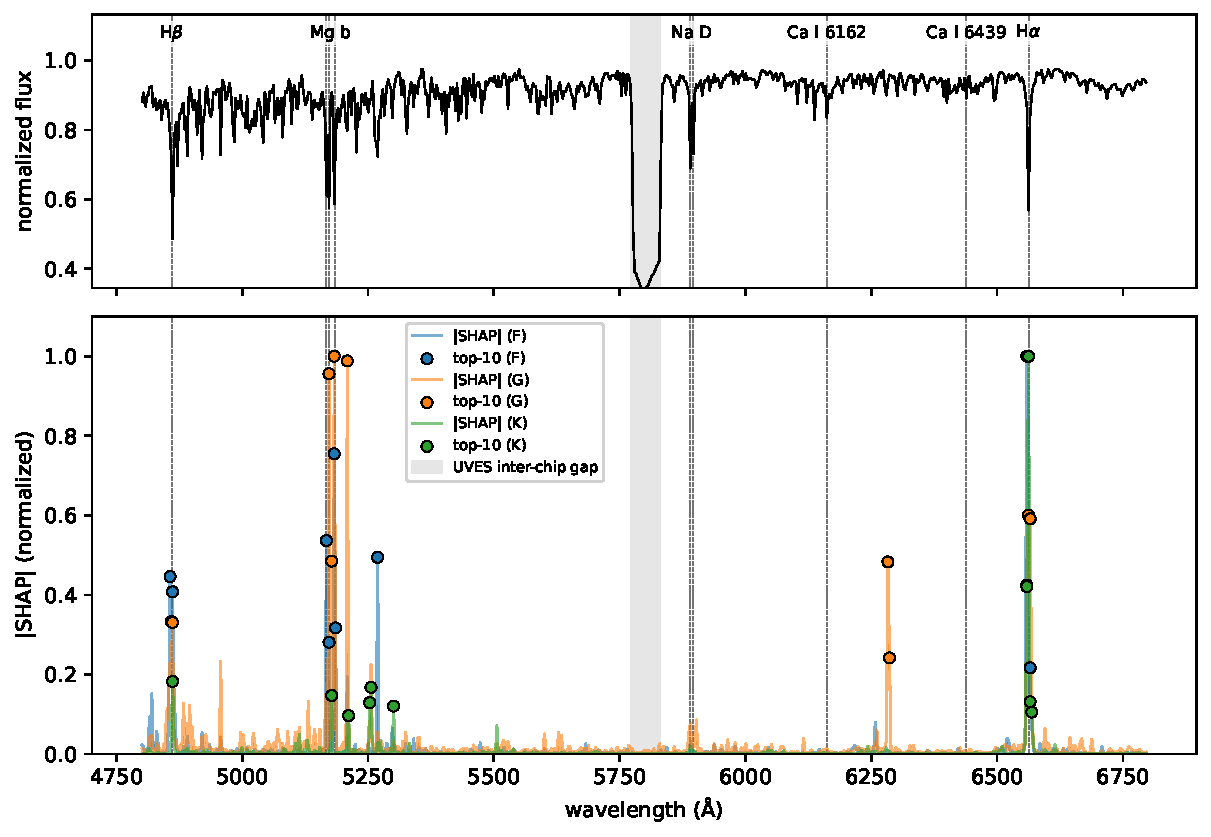
\includegraphics[width=0.92\linewidth]{importance_main.pdf}
\caption{Top: per-bin median normalised spectrum of the G class with the diagnostic-line positions marked and the inter-chip gap shaded. Bottom: normalised mean $|\mathrm{SHAP}|$ per class (F blue, G orange, K green) with the ten largest bins of each class marked. The masked-line ablation results are in Figure~\ref{fig:ablation}.}
\label{fig:importance}
\alttext{Two stacked panels sharing a wavelength axis. The top panel shows the median normalised G-class spectrum with vertical lines at the diagnostic lines and a shaded inter-chip gap. The bottom panel shows the normalised mean absolute SHAP value per class, with sharp peaks at H beta, the Mg b triplet and H alpha, and markers on the ten largest bins of each class.}
\end{figure*}

\begin{figure}[ht]
\centering
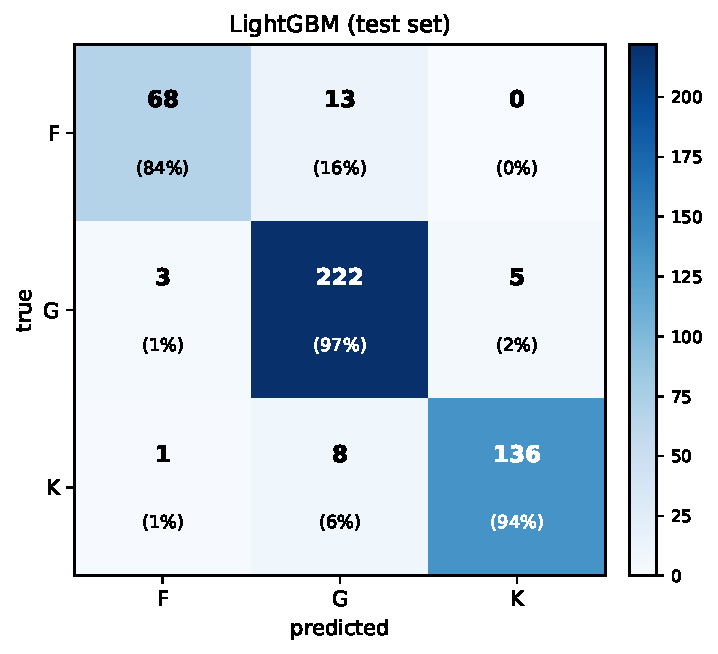
\includegraphics[width=0.55\linewidth]{confusion_matrix_test.pdf}
\caption{Held-out test confusion matrix. Rows are the true class and columns the predicted class, in F--G--K order.}
\label{fig:confusion}
\alttext{Three-by-three confusion matrix of true against predicted class for the held-out test set. Most counts lie on the diagonal; the off-diagonal counts are small and fall between adjacent classes, with almost no confusion between F and K.}
\end{figure}

\end{document}
